\chapter{Visco-elasticity: physics, formulations and FEM } %%%%%%%%%%%%%%%%%%%%%%%%%%%%%%%%%%%%%%%%

The following chapter is based on about a dozen of references:
\begin{itemize}
\item \fullcite{}
\item \fullcite{}
\item \fullcite{bepo10}
\item \fullcite{beps10}
\item \fullcite{chtl13}
\item \fullcite{famc14}
\item \fullcite{daws16}
\item \fullcite{bafg20}
\item \fullcite{}
\item \fullcite{}
\item \fullcite{}
\end{itemize}


One will find in the literature either 'elasto-viscosity' or 'visco-elasticity'.
In what follows I have adopted the former notation with the acronym EV.


\begin{verbatim}
python_codes/fieldstone_64/
python_codes/fieldstone_129/ Visco-elastic materials - Simpson book chapter 12
\end{verbatim}

Let us start by clarifying notations:

\begin{center}
\begin{tabular}{p{6cm}p{2cm}p{2cm}}
\hline
variable name & symbol & unit \\
\hline\hline
full stress tensor & ${\bm \sigma}$ & \si{\pascal}\\
deviatoric stress tensor & ${\bm \tau}$ & \si{\pascal}\\
strain tensor & ${\bm \varepsilon}$ &  - \\
elastic strain tensor & ${\bm \varepsilon}^{\rm e}$ &  - \\
visco-plastic strain tensor & ${\bm \varepsilon}^{\rm vp}$ &  - \\
total strain tensor & ${\bm \varepsilon}^{\rm T}$ &  - \\
strain rate tensor & $\dot{\bm \varepsilon},{\bm \varepsilon}(\vec\upnu)$ & \si{\per\second} \\
anti-symmetric vel gradient & $\dot{\omega},{\bm\omega}(\vec\upnu)$ & \si{\per\second} \\
Lam\'e parameter & $\lambda$ & $\si{\pascal}$ \\
Shear modulus & $\mu(G)$ & $\si{\pascal}$ \\
Bulk modulus & $K$& $\si{\pascal}$\\
Poisson ratio & $\nu$ & -\\
Young's modulus & $E$ & \si{\pascal}\\
... $\xi$ & \\
viscosity & $\eta$ & \si{\pascal\second} \\
displacement & $\vec\upupsilon$ & \si{\meter} \\
velocity & $\vec\upnu$ & \si{\meter\per\second} \\
\hline
\end{tabular}
\end{center}




%==================================================================================================
%==================================================================================================
%==================================================================================================
\section{The physics}

The flow is compressible, but we start from Eq.~(12.40) in the book of Simpson (I here use 
my notations and not those of the book), which only considers the deviatoric part of the 
strain rate tensor and decomposes it into an elastic component and a viscous component:
\begin{eqnarray}
\dot{\bm\varepsilon}^d
&=& \dot{\bm\varepsilon}^{\rm e} + \dot{\bm\varepsilon}^{\rm v} \nn\\
&=&\frac{1}{2\mu} \frac{\partial \bm\tau}{\partial t}
+\frac{1}{2\eta} \bm\tau \nn\\
&\simeq&
\frac{1}{2\mu} \frac{\bm\tau - \bm\tau^0}{\delta t}
+\frac{1}{2\eta} \bm\tau \nn\\
&=&
\frac12 \left( \frac{1}{\mu \delta t} + \frac{1}{\eta} \right) {\bm\tau}
-\frac{1}{2\mu \delta t} \bm\tau^0\nn\\
&=&
\frac12 \frac{ \mu\delta t +\eta}{\mu \delta t \eta}  {\bm\tau}
-\frac{1}{2\mu \delta t} \bm\tau^0
\end{eqnarray}
where ${\bm \tau}^0$ is the already known/previous deviatoric stress tensor. This can be rewritten as
\begin{eqnarray}
\bm\tau 
%&=& 2\left( \frac{1}{\mu \delta t} + \frac{1}{\eta} \right)^{-1} \dot{\bm\varepsilon}^d -2
%\left( \frac{1}{\mu \delta t} + \frac{1}{\eta} \right)^{-1} \frac{1}{2\mu \delta t} \bm\tau^0 
%\nn\\
%&=& 2 \left( \frac{ \mu\delta t +\eta}{\mu \delta t \eta}   \right)^{-1} \dot{\bm\varepsilon}^d -
%2 \left( \frac{\mu\delta t + \eta}{\mu \delta t \eta} \right)^{-1} \frac{1}{2\mu \delta t} \bm\tau^0
%\nn\\
&=&
2  \frac{\mu \delta t \; \eta}{ \mu\delta t +\eta} \dot{\bm\varepsilon}^d 
+
2 \frac{\mu \delta t \; \eta}{\mu\delta t + \eta} \frac{1}{2\mu \delta t} \bm\tau^0
\nn\\
&=&
\frac{2 \mu \delta t \eta}{ \mu\delta t +\eta} \dot{\bm\varepsilon}^d 
+
\frac{ \eta}{\mu\delta t + \eta}  \bm\tau^0 \label{tau_simp1}
\end{eqnarray}
Note that one would often introduce here the effective visco-elastic 
viscosity $\eta^{\rm ve}$ and the Maxwell time $t^M$. However, I shall refrain 
from doing so right now so as to keep as close as possible to the book. 
I will introduce them later.

Defining the mean stress $\sigma_m$ as
\[
\sigma_m = \frac13 {\rm tr}({\bm \sigma})=\frac13(\sigma_{xx}+\sigma_{yy}+\sigma_{zz})
\]
then by definition of the deviatoric stress 
$\bm\tau = {\bm \sigma} - \frac13 {\rm tr}({\bm \sigma}) {\bm 1}= \bm\sigma -\sigma_m {\bm 1} $. 
Also, the viscous deformation is deviatoric so the volume changes
are only due to the elastic deformation and we have\footnote{
In the book it is written as $\sigma_m = 3K \varepsilon_v $}
\[
\sigma_m 
%= 3K \varepsilon_v 
= K \; {\rm tr}({\bm\varepsilon})
\]
Then, assuming $K$ is constant in time,
\[
\frac{\partial\sigma_m}{\partial t} 
\simeq 
\frac{\sigma_m - \sigma_m^0}{\delta t}
= K \; {\rm tr}(\dot{\bm\varepsilon})
\qquad
\Rightarrow
\qquad
\sigma_m \simeq K \; {\rm tr}(\dot{\bm\varepsilon}) \delta t + \sigma_m^0
\]
and then
\[
\bm\tau = \bm\sigma -\sigma_m {\bm 1} 
= \bm\sigma - [K \;  {\rm tr}(\dot{\bm\varepsilon}) \delta t + \sigma_m^0] {\bm 1}
\]
Inserting this in Eq.~\eqref{tau_simp1}
we obtain 
\begin{mdframed}[backgroundcolor=blue!5]
\begin{equation}
\bm \sigma 
= K \; {\rm tr}(\dot{\bm\varepsilon}) \delta t {\bm 1}  +
\frac{2 \mu \eta\delta t}{ \mu\delta t +\eta} \dot{\bm\varepsilon}^d +
\frac{ \eta}{\mu\delta t + \eta}  \bm\tau^0 + \sigma_m^0 {\bm 1}
\label{f129:eq:sigma}
\end{equation}
\end{mdframed}

%==================================================================================================
%==================================================================================================
%==================================================================================================
\section{The weak form}

ToDo







%==================================================================================================
%==================================================================================================
%==================================================================================================
\section{The stress vector}

We can now switch to using a vector representation of the tensors\footnote{We need 
to be extra careful about the strain rate vector $\dot{\vec{\varepsilon}}$ since 
it contains a factor 2 in front of the off diagonal tensor terms, hence the ${\bm C}$ tensor.} 
as it is necessary for implementation in a FEM code:
\begin{eqnarray}
{\bm \sigma} &\rightarrow& \vec{\sigma} \nn\\
{\bm \varepsilon} &\rightarrow& {\bm C} \cdot \vec{\varepsilon} \nn\\
{\bm 1} &\rightarrow& \vec{m} \nn
\end{eqnarray}
with 
\[
\vec{m}=
\left(
\begin{array}{c}
1 \\ 1 \\ 1 \\ 0 \\ 0 \\ 0
\end{array}
\right),
\qquad\quad
{\bm C}=
\left(
\begin{array}{cccccc}
1 & 0 & 0 & 0 & 0 & 0 \\
0 & 1 & 0 & 0 & 0 & 0 \\
0 & 0 & 1 & 0 & 0 & 0 \\
0 & 0 & 0 & 1/2 & 0 & 0 \\
0 & 0 & 0 & 0 & 1/2 & 0 \\
0 & 0 & 0 & 0 & 0 & 1/2 
\end{array}
\right),
\qquad
{\rm and} 
\qquad
\dot{\vec{\varepsilon}}=
\left(
\begin{array}{c}
\dot\varepsilon_{xx}\\ 
\dot\varepsilon_{yy}\\ 
\dot\varepsilon_{zz}\\ 
{\color{teal}2}\dot\varepsilon_{xy} \\ 
{\color{teal}2}\dot\varepsilon_{xz} \\ 
{\color{teal}2}\dot\varepsilon_{yz}
\end{array}
\right).
\]
%so that 
%\[
%\vec{\sigma} = K {\rm tr}(\dot{\bm\varepsilon}) \delta t \vec{m} +
%\frac{2 \mu \delta t}{ \mu\delta t +\eta} \dot{\vec{\bm\varepsilon}}^d -
%\frac{ \eta}{\mu\delta t + \eta}  \bm\tau^0 + \sigma_m^0 \vec{m}
%\]
Also, as we have seen in Eq.~\eqref{eq:el:opla1} we have
$\vec\tau = {\bm I}_d \cdot \vec\sigma$
%and $\vec\varepsilon^d = {\bm I}_d \cdot \vec\varepsilon$
with ${\bm I}_d$ the deviatoric operator:
\[
{\bm I}_d=
\left(
\begin{array}{cccccc}
\frac23 & - \frac13 & - \frac13 & 0 & 0 & 0 \\
-\frac13 & \frac23 & - \frac13  & 0 & 0 & 0\\
-\frac13& - \frac13 & \frac23  & 0 & 0 & 0\\
0&0&0& 1&0 &0  \\
0&0&0&0&1 &0\\
0&0&0&0&0& 1
\end{array}
\right)
\]
so that now Eq.~\eqref{f129:eq:sigma} becomes:

\begin{eqnarray}
\vec{\sigma} 
&=& K \; {\rm tr}(\dot{\bm\varepsilon}) \delta t \;  \vec{m} +
\frac{2 \mu \eta\delta t}{ \mu\delta t +\eta} {\bm I}_d \cdot {\bm C} \cdot\dot{\vec{\bm\varepsilon}} 
+\frac{ \eta}{\mu\delta t + \eta} {\bm I}_d \cdot \bm\sigma^0 + \sigma_m^0 \;  \vec{m} \nn\\
&=& 
\left(
\begin{array}{c}
K \; {\rm tr}(\dot{\bm\varepsilon}) \delta t \\
K \; {\rm tr}(\dot{\bm\varepsilon}) \delta t \\
K \; {\rm tr}(\dot{\bm\varepsilon}) \delta t \\
0 \\ 
0 \\
0
\end{array}
\right)
+
\frac{2 \mu \eta \delta t}{ \mu\delta t +\eta} 
\left(
\begin{array}{cccccc}
\frac23 & - \frac13 & - \frac13 & 0 & 0 & 0 \\
-\frac13 & \frac23 & - \frac13  & 0 & 0 & 0\\
-\frac13& - \frac13 & \frac23  & 0 & 0 & 0\\
0&0&0& 1&0 &0  \\
0&0&0&0&1 &0\\
0&0&0&0&0& 1
\end{array}
\right)
\cdot 
\left(
\begin{array}{cccccc}
1 & 0 & 0 & 0 & 0 & 0 \\
0 & 1 & 0 & 0 & 0 & 0 \\
0 & 0 & 1 & 0 & 0 & 0 \\
0 & 0 & 0 & 1/2 & 0 & 0 \\
0 & 0 & 0 & 0 & 1/2 & 0 \\
0 & 0 & 0 & 0 & 0 & 1/2 
\end{array}
\right)
\cdot
\left(
\begin{array}{c}
\dot\varepsilon_{xx}\\ 
\dot\varepsilon_{yy}\\ 
\dot\varepsilon_{zz}\\ 
{\color{teal}2}\dot\varepsilon_{xy} \\
{\color{teal}2}\dot\varepsilon_{xz} \\
{\color{teal}2}\dot\varepsilon_{yz}
\end{array}
\right) 
\nn\\
&+& 
\frac{ \eta}{\mu\delta t + \eta}
\left(
\begin{array}{cccccc}
\frac23 & - \frac13 & - \frac13 & 0 & 0 & 0 \\
-\frac13 & \frac23 & - \frac13  & 0 & 0 & 0\\
-\frac13& - \frac13 & \frac23  & 0 & 0 & 0\\
0&0&0& 1&0 &0  \\
0&0&0&0&1 &0\\
0&0&0&0&0& 1
\end{array}
\right)
\cdot
\left(
\begin{array}{c}
\sigma_{xx}^0\\ 
\sigma_{yy}^0\\ 
\sigma_{zz}^0\\ 
\sigma_{xy}^0 \\
\sigma_{xz}^0 \\
\sigma_{yz}^0
\end{array}
\right) 
+
\sigma_m^0 
\left(
\begin{array}{c}
1\\
1\\
1\\
0\\
0\\
0
\end{array}
\right) 
\nn\\
&=&
\delta t
\left(
\begin{array}{cccccc}
K & K & K & 0 & 0 & 0\\ 
K & K & K & 0 & 0 & 0\\ 
K & K & K & 0 & 0 & 0\\ 
0 & 0 & 0 & 0 & 0 & 0 \\
0 & 0 & 0 & 0 & 0 & 0 \\
0 & 0 & 0 & 0 & 0 & 0 
\end{array}
\right)
\cdot
\left(
\begin{array}{c}
\dot\varepsilon_{xx}\\ 
\dot\varepsilon_{yy}\\ 
\dot\varepsilon_{zz}\\ 
{\color{teal}2}\dot\varepsilon_{xy} \\ 
{\color{teal}2}\dot\varepsilon_{xz} \\ 
{\color{teal}2}\dot\varepsilon_{yz}
\end{array}
\right) 
+
\frac{2 \mu  \eta\delta t}{ \mu\delta t +\eta} 
\left(
\begin{array}{cccccc}
\frac23 & - \frac13 & - \frac13 & 0 & 0 & 0 \\
-\frac13 & \frac23 & - \frac13  & 0 & 0 & 0\\
-\frac13& - \frac13 & \frac23  & 0 & 0 & 0\\
0&0&0& 1/{\color{teal}2}&0 &0  \\
0&0&0&0&1/{\color{teal}2} &0\\
0&0&0&0&0& 1/{\color{teal}2}
\end{array}
\right)
\cdot
\left(
\begin{array}{c}
\dot\varepsilon_{xx}\\ 
\dot\varepsilon_{yy}\\ 
\dot\varepsilon_{zz}\\ 
{\color{teal}2}\dot\varepsilon_{xy} \\ 
{\color{teal}2}\dot\varepsilon_{xz} \\ 
{\color{teal}2}\dot\varepsilon_{yz}
\end{array}
\right) 
\nn\\
&+& 
\frac{ \eta}{\mu\delta t + \eta}
\left(
\begin{array}{cccccc}
\frac23 & - \frac13 & - \frac13 & 0 & 0 & 0 \\
-\frac13 & \frac23 & - \frac13  & 0 & 0 & 0\\
-\frac13& - \frac13 & \frac23  & 0 & 0 & 0\\
0&0&0& 1&0 &0  \\
0&0&0&0&1 &0\\
0&0&0&0&0& 1
\end{array}
\right)
\cdot
\left(
\begin{array}{c}
\sigma_{xx}^0\\ 
\sigma_{yy}^0\\ 
\sigma_{zz}^0\\ 
\sigma_{xy}^0 \\
\sigma_{xz}^0 \\
\sigma_{yz}^0
\end{array}
\right) 
+
\left(
\begin{array}{cccccc}
\frac13 & \frac13 & \frac13 & 0 & 0 & 0 \\
\frac13 & \frac13 & \frac13 & 0 & 0 & 0 \\
\frac13 & \frac13 & \frac13 & 0 & 0 & 0 \\
0 &0 &0 & 0 & 0 & 0 \\
0 &0 &0 & 0 & 0 & 0 \\
0 &0 &0 & 0 & 0 & 0 
\end{array}
\right) 
\cdot
\left(
\begin{array}{c}
\sigma_{xx}^0\\ 
\sigma_{yy}^0\\ 
\sigma_{zz}^0\\ 
\sigma_{xy}^0 \\
\sigma_{xz}^0 \\
\sigma_{yz}^0
\end{array}
\right) 
\nn\\
&=& 
\delta t
\left[
\left(
\begin{array}{cccccc}
K & K & K & 0 & 0 & 0\\ 
K & K & K & 0 & 0 & 0\\ 
K & K & K & 0 & 0 & 0\\ 
0 & 0 & 0 & 0 & 0 & 0 \\
0 & 0 & 0 & 0 & 0 & 0 \\
0 & 0 & 0 & 0 & 0 & 0 
\end{array}
\right)
+
\frac{2 \mu \eta}{ \mu\delta t +\eta} 
\left(
\begin{array}{cccccc}
\frac23 & - \frac13 & - \frac13 & 0 & 0 & 0 \\
-\frac13 & \frac23 & - \frac13  & 0 & 0 & 0\\
-\frac13& - \frac13 & \frac23  & 0 & 0 & 0\\
0&0&0& 1/{\color{teal}2}&0 &0  \\
0&0&0&0&1/{\color{teal}2} &0\\
0&0&0&0&0& 1/{\color{teal}2}
\end{array}
\right)
\right]
\cdot
\left(
\begin{array}{c}
\dot\varepsilon_{xx}\\ 
\dot\varepsilon_{yy}\\ 
\dot\varepsilon_{zz}\\ 
{\color{teal}2}\dot\varepsilon_{xy} \\ 
{\color{teal}2}\dot\varepsilon_{xz} \\ 
{\color{teal}2}\dot\varepsilon_{yz}
\end{array}
\right) 
\nn\\
&+& 
\left[
\frac{ \eta}{\mu\delta t + \eta}
\left(
\begin{array}{cccccc}
\frac23 & - \frac13 & - \frac13 & 0 & 0 & 0 \\
-\frac13 & \frac23 & - \frac13  & 0 & 0 & 0\\
-\frac13& - \frac13 & \frac23  & 0 & 0 & 0\\
0&0&0& 1&0 &0  \\
0&0&0&0&1 &0\\
0&0&0&0&0& 1
\end{array}
\right)
+
\left(
\begin{array}{cccccc}
\frac13 & \frac13 & \frac13 & 0 & 0 & 0 \\
\frac13 & \frac13 & \frac13 & 0 & 0 & 0 \\
\frac13 & \frac13 & \frac13 & 0 & 0 & 0 \\
0 &0 &0 & 0 & 0 & 0 \\
0 &0 &0 & 0 & 0 & 0 \\
0 &0 &0 & 0 & 0 & 0 
\end{array}
\right) 
\right]
\cdot
\left(
\begin{array}{c}
\sigma_{xx}^0\\ 
\sigma_{yy}^0\\ 
\sigma_{zz}^0\\ 
\sigma_{xy}^0 \\
\sigma_{xz}^0 \\
\sigma_{yz}^0
\end{array}
\right) \nn\\
&=& 
\delta t
\left(
\begin{array}{cccccc}
K + \frac{4\mu \eta/3}{\mu \delta t + \eta} &
K - \frac{2\mu \eta/3}{\mu \delta t + \eta} &
K - \frac{2\mu \eta/3}{\mu \delta t + \eta} &
0 &0 & 0 \\
K - \frac{2\mu \eta/3}{\mu \delta t + \eta} &
K + \frac{4\mu \eta/3}{\mu \delta t + \eta} &
K - \frac{2\mu \eta/3}{\mu \delta t + \eta} &
0 &0 & 0 \\
K - \frac{2\mu \eta/3}{\mu \delta t + \eta} &
K - \frac{2\mu \eta/3}{\mu \delta t + \eta} &
K + \frac{4\mu \eta/3}{\mu \delta t + \eta} &
0 &0 & 0 \\
0 & 0 & 0 & \frac{\mu \eta }{\mu \delta t + \eta} & 0 & 0 \\
0 & 0 & 0 & 0 & \frac{\mu \eta }{\mu \delta t + \eta} & 0  \\
0 & 0 & 0 & 0 & 0 & \frac{\mu \eta }{\mu \delta t + \eta} 
\end{array}
\right)
\cdot
\left(
\begin{array}{c}
\dot\varepsilon_{xx}\\ 
\dot\varepsilon_{yy}\\ 
\dot\varepsilon_{zz}\\ 
{\color{teal}2}\dot\varepsilon_{xy} \\ 
{\color{teal}2}\dot\varepsilon_{xz} \\ 
{\color{teal}2}\dot\varepsilon_{yz}
\end{array}
\right) 
\nn\\
&+&
\left(
\begin{array}{cccccc}
\frac13\frac{3\eta + \mu \delta t}{\mu\delta t+\eta} & 
\frac13\frac{\mu \delta t}{\mu\delta t+\eta} & 
\frac13\frac{\mu \delta t}{\mu\delta t+\eta} & 0 & 0 & 0\\
\frac13\frac{\mu \delta t}{\mu\delta t+\eta} & 
\frac13\frac{3\eta + \mu \delta t}{\mu\delta t+\eta} & 
\frac13\frac{\mu \delta t}{\mu\delta t+\eta} & 0 & 0 & 0\\
\frac13\frac{\mu \delta t}{\mu\delta t+\eta} & 
\frac13\frac{\mu \delta t}{\mu\delta t+\eta} & 
\frac13\frac{3\eta + \mu \delta t}{\mu\delta t+\eta} & 0 & 0 & 0\\
0 & 0 & 0 & \frac{ \eta}{\mu\delta t + \eta} & 0 & 0 \\
0 & 0 & 0 & 0 & \frac{ \eta}{\mu\delta t + \eta} & 0  \\
0 & 0 & 0 & 0 & 0 & \frac{ \eta}{\mu\delta t + \eta} 
\end{array}
\right)
\cdot
\left(
\begin{array}{c}
\sigma_{xx}^0\\ 
\sigma_{yy}^0\\ 
\sigma_{zz}^0\\ 
\sigma_{xy}^0 \\
\sigma_{xz}^0 \\
\sigma_{yz}^0
\end{array}
\right) \label{simpson3D}
\end{eqnarray}




%------------------------------------------------------------------------------
\subsection{In Plane strain}
We start again from Eq.~\eqref{f129:eq:sigma}:
\begin{eqnarray}
\bm \sigma 
&=& 
K {\rm tr}(\dot{\bm\varepsilon}) \delta t {\bm 1}  +
\frac{2 \mu \eta\delta t}{ \mu\delta t +\eta} \dot{\bm\varepsilon}^d +
\frac{ \eta}{\mu\delta t + \eta}  \bm\tau^0 + \sigma_m^0 {\bm 1}
\end{eqnarray}

In plane strain, assuming deformation occurs in the $xy$-plane, we have 
$\dot\varepsilon_{zz}=\dot\varepsilon_{xz}=\dot\varepsilon_{yz}=0$ and 
$\sigma_{xz}=\sigma_{yz}=0$ (Note that $\sigma_{zz}\ne 0$ !). Furthermore 
we have\footnote{Since the spring and dashpot are in series, they are under 
the same stress} the viscous strain rate given by:
\[
\dot{\bm\varepsilon}_v
= \frac{1}{2\eta} {\bm \tau}
= \frac{1}{2\eta} \left( {\bm \sigma} - \frac13 {\rm tr}(\bm\sigma) {\bm 1} \right)
\]
Looking at the $zz$ component of the above equation yields
\[
\dot{\varepsilon}_{v,zz} = \frac{1}{2\eta} \frac13 (2\sigma_{zz}-\sigma_{xx}-\sigma_{yy})
\]
Assuming $\dot{\varepsilon}_{v,zz}=0$ (stricly speaking only the total strain  $\dot\varepsilon_{zz}=0$ but it is then logical to assume that the 
$zz$-strain rate for both mechanisms is zero simultaneously), we obtain
$\sigma_{zz}=\frac12 (\sigma_{xx}+\sigma_{yy})$.
In that sense we can discard the $\sigma_{zz}$ equation since it is 
not unknown anymore in this case.

Note that the mean stress then becomes
\[
\sigma_m 
= \frac{1}{3}(\sigma_{xx}+\sigma_{yy}+\sigma_{zz})
= \frac{1}{3}(\sigma_{xx}+\sigma_{yy}+\frac12(\sigma_{xx}+\sigma_{yy}))
= \frac{1}{2}(\sigma_{xx}+\sigma_{yy})
\]


We are left with the $\sigma_{xx}$, $\sigma_{yy}$ and $\sigma_{xy}$
equations. All we have to do is select the 1st, 2nd and 4th lines and 
columns of the vectors/matrices in Eq.~\eqref{simpson3D}:

\[
\left(
\begin{array}{c}
\sigma_{xx}\\ 
\sigma_{yy}\\ 
\sigma_{xy} 
\end{array}
\right)
=
\delta t
\left(
\begin{array}{ccc}
K + \frac{4\mu \eta/3}{\mu \delta t + \eta} &
K - \frac{2\mu \eta/3}{\mu \delta t + \eta} &
0 \\
K - \frac{2\mu \eta/3}{\mu \delta t + \eta} &
K + \frac{4\mu \eta/3}{\mu \delta t + \eta} &
0  \\
0 & 0 & \frac{\mu \eta }{\mu \delta t + \eta}  \\
\end{array}
\right)
\cdot
\left(
\begin{array}{c}
\dot\varepsilon_{xx}\\ 
\dot\varepsilon_{yy}\\ 
{\color{teal}2}\dot\varepsilon_{xy} 
\end{array}
\right) 
+
\left(
\begin{array}{cccccc}
\frac13\frac{3\eta + \mu \delta t}{\mu\delta t+\eta} & 
\frac13\frac{\mu \delta t}{\mu\delta t+\eta} & 
0\\
\frac13\frac{\mu \delta t}{\mu\delta t+\eta} & 
\frac13\frac{3\eta + \mu \delta t}{\mu\delta t+\eta} & 
0\\
0 & 0 & \frac{ \eta}{\mu\delta t + \eta}  
\end{array}
\right)
\cdot
\left(
\begin{array}{c}
\sigma_{xx}^0\\ 
\sigma_{yy}^0\\ 
\sigma_{xy}^0 
\end{array}
\right) 
\]
or,
\begin{mdframed}[backgroundcolor=blue!5]
{\small
\begin{equation}
\left(
\begin{array}{c}
\sigma_{xx}\\ 
\sigma_{yy}\\ 
\sigma_{xy} 
\end{array}
\right)
=
\left(
\begin{array}{ccc}
\frac{\delta t(4\mu \eta + 3K \eta+ 3K \mu\delta t)}{3(\mu \delta t + \eta)} &
\frac{\delta t(3K \eta+ 3K \mu\delta t - 2\mu \eta)}{3(\mu \delta t + \eta)} &
0 \\
\frac{\delta t(3K \eta+ 3K \mu\delta t  - 2\mu \eta)}{3(\mu \delta t + \eta)}&
\frac{\delta t(4\mu \eta + 3K \eta+ 3K \mu\delta t)}{3(\mu \delta t + \eta)} &
0  \\
0 & 0 & \frac{\mu \eta \delta t }{\mu \delta t + \eta}  \\
\end{array}
\right)
\cdot
\left(
\begin{array}{c}
\dot\varepsilon_{xx}\\ 
\dot\varepsilon_{yy}\\ 
{\color{teal}2}\dot\varepsilon_{xy} 
\end{array}
\right) 
+
\left(
\begin{array}{cccccc}
\frac13\frac{3\eta + \mu \delta t}{\mu\delta t+\eta} & 
\frac13\frac{\mu \delta t}{\mu\delta t+\eta} & 
0\\
\frac13\frac{\mu \delta t}{\mu\delta t+\eta} & 
\frac13\frac{3\eta + \mu \delta t}{\mu\delta t+\eta} & 
0\\
0 & 0 & \frac{ \eta}{\mu\delta t + \eta}  
\end{array}
\right)
\cdot
\left(
\begin{array}{c}
\sigma_{xx}^0\\ 
\sigma_{yy}^0\\ 
\sigma_{xy}^0 
\end{array}
\right) 
\label{eq_129_2D}
\end{equation}
}
\end{mdframed}

In order to compare this with the book's equations, I rewrite the above equation with the 
book's notations ($\mu \rightarrow G$, $\eta\rightarrow \mu$):
{\small
\begin{eqnarray}
\left(
\begin{array}{c}
\sigma_{xx}\\ 
\sigma_{yy}\\ 
\sigma_{xy} 
\end{array}
\right)
=
\underbrace{
\left(
\begin{array}{ccc}
\frac{\delta t(4G \mu + 3K \mu+ 3K G\delta t)}{3(G \delta t + \mu)} &
\frac{\delta t(3K \mu+ 3K G\delta t - 2G \mu)}{3(G \delta t + \mu)} &
0 \\
\frac{\delta t(3K \mu+ 3K G\delta t  - 2G \mu)}{3(G \delta t + \mu)}&
\frac{\delta t(4G \mu + 3K \mu+ 3K G\delta t)}{3(G \delta t + \mu)} &
0  \\
0 & 0 & \frac{G \mu \delta t }{G \delta t + \mu}  \\
\end{array}
\right)
}_{\tilde{\bm D}}
\!
\cdot\!
\left(
\begin{array}{c}
\dot\varepsilon_{xx}\\ 
\dot\varepsilon_{yy}\\ 
{\color{teal}2}\dot\varepsilon_{xy} 
\end{array}
\right) 
+
\underbrace{
\left(
\begin{array}{cccccc}
\frac{3\mu + G \delta t}{3(G\delta t+\mu)} & 
\frac{G \delta t}{3(G\delta t+\mu)} & 
0\\
\frac{G \delta t}{3(G\delta t+\mu)} & 
\frac{3\mu + G \delta t}{3(G\delta t+\mu)} & 
0\\
0 & 0 & \frac{ \mu}{G\delta t + \eta}  
\end{array}
\right)
}_{\tilde{\bm D}_s}
\!\cdot\!
\left(
\begin{array}{c}
\sigma_{xx}^0\\ 
\sigma_{yy}^0\\ 
\sigma_{xy}^0 
\end{array}
\right) 
\nonumber
\end{eqnarray}
}


\begin{center}
\fbox{
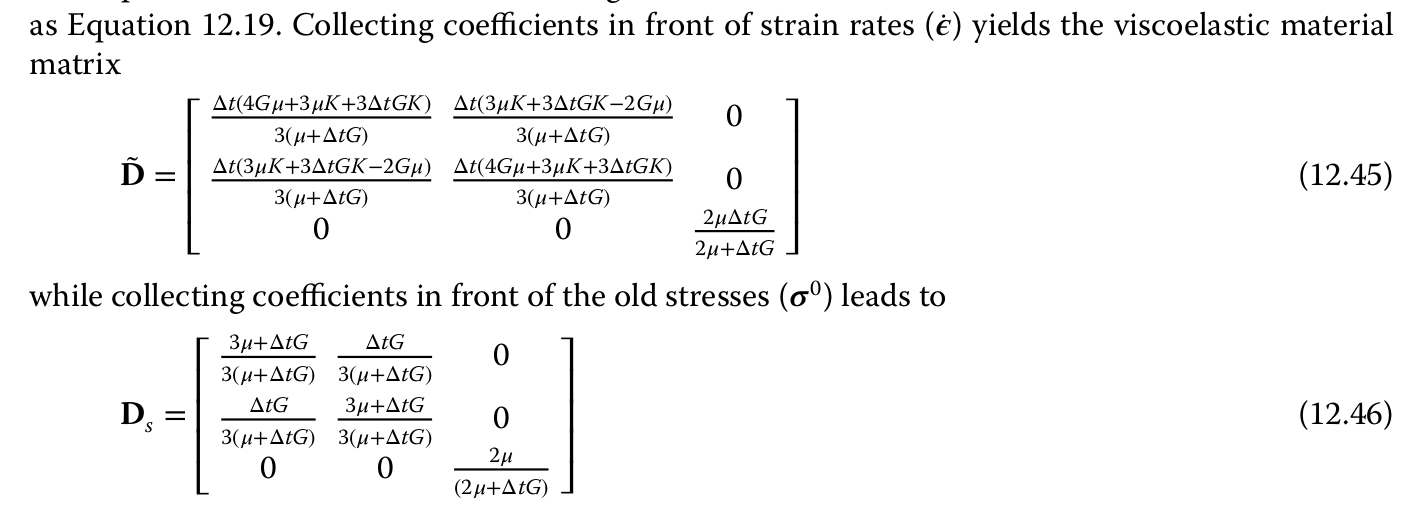
\includegraphics[width=17cm]{python_codes/fieldstone_129/images/simpson_1}}\\
{\captionfont Taken from the book.}
\end{center}

A few remarks:
\begin{itemize}
\item 
Good news, I agree with the book's equations except for the (3,3)
term which in my opinion is {\color{red} missing a factor 2} in front of 
the $\Delta t G$ of the denominator.
I will need an analytical benchmark to sort this out.
\item 
Also I obtain  $\vec\sigma= \tilde{\bm D} \cdot \dot{\vec{\varepsilon}} + {\bm D}_s \cdot \vec{\sigma}^0$ which is coherent with Eq.~(12.19) of the book but the book has a minus sign in front of ${\bm D}_s$ on page 188.
\item 
In any case the book is missing a discussion about the 'disappearance' of $\sigma_{yy}$ after Eq.~(12.33).
Also Eq.~(12.39) should probably showcase a factor 2 in front of
the $xz$ term.
\item The time derivative in Eq.~(12.40) is in fact the  co-rotational (Jaumann) time derivative of the deviatoric stress tensor. What is presented here is a simplification, which is ok because a Lagrangian approach is taken?
\end{itemize}










%------------------------------------------------------------------------------
%------------------------------------------------------------------------------
\subsection{Using an effective viscosity}

Let us recall the following matrices
\[
{\bm \Lambda}=
\left(
\begin{array}{cccccc}
2 & 0 & 0 & 0 & 0 & 0 \\
0 & 2 & 0 & 0 & 0 & 0 \\
0 & 0 & 2 & 0 & 0 & 0 \\
0 & 0 & 0 & 1 & 0 & 0 \\
0 & 0 & 0 & 0 & 1 & 0 \\
0 & 0 & 0 & 0 & 0 & 1 
\end{array}
\right)
\qquad
{\bm \Lambda}^d
=
\left(
\begin{array}{cccccc}
\frac43 & - \frac23 & - \frac23 & 0 & 0 & 0 \\
-\frac23 & \frac43 & - \frac23  & 0 & 0 & 0\\
-\frac23& - \frac23 & \frac43  & 0 & 0 & 0\\
0&0&0& 1&0 &0  \\
0&0&0&0&1 &0\\
0&0&0&0&0& 1
\end{array}
\right)
\]
\[
\tilde{\bm \Lambda}^d
=
\left(
\begin{array}{cccccc}
\frac23 & - \frac13 & - \frac13 & 0 & 0 & 0 \\
-\frac13 & \frac23 & - \frac13  & 0 & 0 & 0\\
-\frac13& - \frac13 & \frac23  & 0 & 0 & 0\\
0&0&0& 1&0 &0  \\
0&0&0&0&1 &0\\
0&0&0&0&0& 1
\end{array}
\right)
\qquad
{\bm \Xi}=
\left(
\begin{array}{cccccc}
1 & 1 & 1 & 0 & 0 & 0\\ 
1 & 1 & 1 & 0 & 0 & 0\\ 
1 & 1 & 1 & 0 & 0 & 0\\ 
0 & 0 & 0 & 0 & 0 & 0 \\
0 & 0 & 0 & 0 & 0 & 0 \\
0 & 0 & 0 & 0 & 0 & 0 
\end{array}
\right)
\]

It is common to find in the literature the so-called effective 
viscosity $\eta_{\rm ve}$ defined as 
\[
\eta_{\rm ve}
=\frac{\eta \delta t}{\delta t + \eta/\mu}
=\frac{\eta}{1 + t_M/\delta t}
=\frac{\mu\eta \delta t}{\mu \delta t + \eta}
\]
%and 
%\[
%\eta_{eff}' = \frac{\eta_{eff}}{\mu\delta t}
%\]
Then 
\begin{eqnarray}
\bm \sigma 
&=& 
K {\rm tr}(\dot{\bm\varepsilon}) \delta t {\bm 1}  +
2\eta_{\rm ve} \dot{\bm\varepsilon}^d +
\frac{ \eta_{\rm ve}}{\mu\delta t}  \bm\tau^0 + \sigma_m^0 {\bm 1}
\end{eqnarray}



\begin{eqnarray}
\vec{\sigma} 
&=& K {\rm tr}(\dot{\bm\varepsilon}) \delta t \vec{m} +
2\eta_{\rm ve} {\bm I}_d \cdot {\bm C} \cdot\dot{\vec{\bm\varepsilon}} 
+\frac{\eta_{\rm ve}}{\mu\delta t} {\bm I}_d \cdot \vec\sigma^0 + \sigma_m^0 \vec{m} \nn\\
&=& 
\left(
\begin{array}{c}
K {\rm tr}(\dot{\bm\varepsilon}) \delta t \\
K {\rm tr}(\dot{\bm\varepsilon}) \delta t \\
K {\rm tr}(\dot{\bm\varepsilon}) \delta t \\
0 \\ 
0 \\
0
\end{array}
\right)
+
2\eta_{\rm ve}
\left(
\begin{array}{cccccc}
\frac23 & - \frac13 & - \frac13 & 0 & 0 & 0 \\
-\frac13 & \frac23 & - \frac13  & 0 & 0 & 0\\
-\frac13& - \frac13 & \frac23  & 0 & 0 & 0\\
0&0&0& 1&0 &0  \\
0&0&0&0&1 &0\\
0&0&0&0&0& 1
\end{array}
\right)
\cdot 
\left(
\begin{array}{cccccc}
1 & 0 & 0 & 0 & 0 & 0 \\
0 & 1 & 0 & 0 & 0 & 0 \\
0 & 0 & 1 & 0 & 0 & 0 \\
0 & 0 & 0 & 1/2 & 0 & 0 \\
0 & 0 & 0 & 0 & 1/2 & 0 \\
0 & 0 & 0 & 0 & 0 & 1/2 
\end{array}
\right)
\cdot
\left(
\begin{array}{c}
\dot\varepsilon_{xx}\\ 
\dot\varepsilon_{yy}\\ 
\dot\varepsilon_{zz}\\ 
{\color{teal}2}\dot\varepsilon_{xy} \\
{\color{teal}2}\dot\varepsilon_{xz} \\
{\color{teal}2}\dot\varepsilon_{yz}
\end{array}
\right) 
\nn\\
&+& 
\frac{\eta_{\rm ve}}{\mu\delta t}
\left(
\begin{array}{cccccc}
\frac23 & - \frac13 & - \frac13 & 0 & 0 & 0 \\
-\frac13 & \frac23 & - \frac13  & 0 & 0 & 0\\
-\frac13& - \frac13 & \frac23  & 0 & 0 & 0\\
0&0&0& 1&0 &0  \\
0&0&0&0&1 &0\\
0&0&0&0&0& 1
\end{array}
\right)
\cdot
\left(
\begin{array}{c}
\sigma_{xx}^0\\ 
\sigma_{yy}^0\\ 
\sigma_{zz}^0\\ 
\sigma_{xy}^0 \\
\sigma_{xz}^0 \\
\sigma_{yz}^0
\end{array}
\right) 
+
\sigma_m^0 
\left(
\begin{array}{c}
1\\
1\\
1\\
0\\
0\\
0
\end{array}
\right) 
\nn\\
&=&
\delta t
\left(
\begin{array}{cccccc}
K & K & K & 0 & 0 & 0\\ 
K & K & K & 0 & 0 & 0\\ 
K & K & K & 0 & 0 & 0\\ 
0 & 0 & 0 & 0 & 0 & 0 \\
0 & 0 & 0 & 0 & 0 & 0 \\
0 & 0 & 0 & 0 & 0 & 0 
\end{array}
\right)
\cdot
\left(
\begin{array}{c}
\dot\varepsilon_{xx}\\ 
\dot\varepsilon_{yy}\\ 
\dot\varepsilon_{zz}\\ 
{\color{teal}2}\dot\varepsilon_{xy} \\ 
{\color{teal}2}\dot\varepsilon_{xz} \\ 
{\color{teal}2}\dot\varepsilon_{yz}
\end{array}
\right) 
+
2\eta_{\rm ve}
\left(
\begin{array}{cccccc}
\frac23 & - \frac13 & - \frac13 & 0 & 0 & 0 \\
-\frac13 & \frac23 & - \frac13  & 0 & 0 & 0\\
-\frac13& - \frac13 & \frac23  & 0 & 0 & 0\\
0&0&0& 1/{\color{teal}2}&0 &0  \\
0&0&0&0&1/{\color{teal}2} &0\\
0&0&0&0&0& 1/{\color{teal}2}
\end{array}
\right)
\cdot
\left(
\begin{array}{c}
\dot\varepsilon_{xx}\\ 
\dot\varepsilon_{yy}\\ 
\dot\varepsilon_{zz}\\ 
{\color{teal}2}\dot\varepsilon_{xy} \\ 
{\color{teal}2}\dot\varepsilon_{xz} \\ 
{\color{teal}2}\dot\varepsilon_{yz}
\end{array}
\right) 
\nn\\
&+& 
\frac{\eta_{\rm ve}}{\mu\delta t}
\left(
\begin{array}{cccccc}
\frac23 & - \frac13 & - \frac13 & 0 & 0 & 0 \\
-\frac13 & \frac23 & - \frac13  & 0 & 0 & 0\\
-\frac13& - \frac13 & \frac23  & 0 & 0 & 0\\
0&0&0& 1&0 &0  \\
0&0&0&0&1 &0\\
0&0&0&0&0& 1
\end{array}
\right)
\cdot
\left(
\begin{array}{c}
\sigma_{xx}^0\\ 
\sigma_{yy}^0\\ 
\sigma_{zz}^0\\ 
\sigma_{xy}^0 \\
\sigma_{xz}^0 \\
\sigma_{yz}^0
\end{array}
\right) 
+
\left(
\begin{array}{cccccc}
\frac13 & \frac13 & \frac13 & 0 & 0 & 0 \\
\frac13 & \frac13 & \frac13 & 0 & 0 & 0 \\
\frac13 & \frac13 & \frac13 & 0 & 0 & 0 \\
0 &0 &0 & 0 & 0 & 0 \\
0 &0 &0 & 0 & 0 & 0 \\
0 &0 &0 & 0 & 0 & 0 
\end{array}
\right) 
\cdot
\left(
\begin{array}{c}
\sigma_{xx}^0\\ 
\sigma_{yy}^0\\ 
\sigma_{zz}^0\\ 
\sigma_{xy}^0 \\
\sigma_{xz}^0 \\
\sigma_{yz}^0
\end{array}
\right) 
\nn\\
&=& 
\left[
K \delta t {\bm \Xi}
+
\eta_{\rm ve} {\bm \Lambda}^d
\right]
\cdot
\left(
\begin{array}{c}
\dot\varepsilon_{xx}\\ 
\dot\varepsilon_{yy}\\ 
\dot\varepsilon_{zz}\\ 
{\color{teal}2}\dot\varepsilon_{xy} \\ 
{\color{teal}2}\dot\varepsilon_{xz} \\ 
{\color{teal}2}\dot\varepsilon_{yz}
\end{array}
\right) 
+ 
\left[
\frac{\eta_{\rm ve}}{\mu\delta t}
\tilde{\bm\Lambda}^d
+
\frac13 {\bm \Xi}
\right]
\cdot
\left(
\begin{array}{c}
\sigma_{xx}^0\\ 
\sigma_{yy}^0\\ 
\sigma_{zz}^0\\ 
\sigma_{xy}^0 \\
\sigma_{xz}^0 \\
\sigma_{yz}^0
\end{array}
\right) 
\label{simpson3D_b}
\end{eqnarray}







\begin{mdframed}[backgroundcolor=blue!5]
\[
\vec\sigma = 
\left(
K \delta t {\bm \Xi}
+
\eta_{\rm ve} {\bm \Lambda}^d
\right)
\cdot
\dot{\vec{\varepsilon}}
+
\left[
\frac{\eta_{\rm ve}}{\mu\delta t}
\tilde{\bm\Lambda}^d
+
\frac13 {\bm \Xi}
\right]
\cdot
\vec\sigma_0
\]
\end{mdframed}

We see that this yields much more compact notations
than the section above.



%----------------------------------------------
\subsection{End member: infinite viscosity}
In this case the Maxwell time $t_M=\eta/\mu$ is very large.
We have $\eta/\mu >> \delta t$ so that $\eta_{\rm ve} 
\rightarrow \mu \delta t$. This makes sense, infinite 
viscosity means that the dashpot behaves as a rigid block 
and its viscosity will not play a role in the deformation
and it'll propagate the stress to the spring.

Then the rhs of the equation just above becomes: 
\[
\frac{\eta_{\rm ve}}{\mu \delta t} \tilde{\bm\Lambda}^d + 
\frac13 {\bm\Xi} 
\rightarrow
\tilde{\bm\Lambda}^d + 
\frac13 {\bm\Xi} 
=
{\bm I}
\]

Then
\begin{eqnarray}
\vec{\sigma}
&=&
\left(
K \delta t {\bm \Xi}
+
\mu \delta t {\bm \Lambda}^d
\right)
\cdot
\dot{\vec{\varepsilon}}
+
\vec{\sigma}_0 \nn\\
&=& 
\delta t (K  {\bm \Xi}
+ \mu  {\bm \Lambda}^d) \cdot 
\dot{\vec{\varepsilon}}
+
\vec{\sigma}_0 
\end{eqnarray}
or,
\[
\frac{\vec\sigma - \vec\sigma_0}{\delta t}
=(
K  {\bm \Xi}
+ \mu  {\bm \Lambda}^d)
\cdot \dot{\vec{\varepsilon}}
\]
which is a discretised form of the time derivative of Eq.~(XYZ). It all makes sense, we recover a purely 
elastic formulation!


%----------------------------------------------
\subsection{End member: infinite shear modulus}
In this case the Maxwell time is very small and the effective
viscosity tends to the real viscosity and also  
\[
\frac{\eta_{\rm ve}}{\mu \delta t} 
\rightarrow 
\frac{\eta}{\mu \delta t} 
\rightarrow 0
\]

Then

\begin{eqnarray}
\vec{\sigma}
&=&
\left(
\underbrace{K \delta t}_{\lambda} {\bm \Xi}
+
\eta {\bm \Lambda}^d
\right)
\cdot
\dot{\vec{\varepsilon}}
+
\vec{\sigma}_0 
= 
\lambda 
\left(
\begin{array}{cccccc}
1 & 1 & 1 & 0 & 0 & 0\\ 
1 & 1 & 1 & 0 & 0 & 0\\ 
1 & 1 & 1 & 0 & 0 & 0\\ 
0 & 0 & 0 & 0 & 0 & 0 \\
0 & 0 & 0 & 0 & 0 & 0 \\
0 & 0 & 0 & 0 & 0 & 0 
\end{array}
\right)
+ 
\eta 
\left(
\begin{array}{cccccc}
\frac43 & - \frac23 & - \frac23 & 0 & 0 & 0 \\
-\frac23 & \frac43 & - \frac23  & 0 & 0 & 0\\
-\frac23& - \frac23 & \frac43  & 0 & 0 & 0\\
0&0&0& 1&0 &0  \\
0&0&0&0&1 &0\\
0&0&0&0&0& 1
\end{array}
\right)
\cdot
\dot{\vec{\varepsilon}}
\end{eqnarray}
We notice that 
${\bm \Lambda}^d$ is identical to the matrix ${\bm C}^d$ in \eqref{eq:chap6:mixed:Cd}.
Also, this formulation looks identical to the standard penalty formulation 
(see Section~\ref{sec_penalty}), except for 
the $\vec{\sigma}_0$ term which accounts for the initial stress.

This also probably means that reduced integration can/should be done ?


%---------------------------------------------------
\subsection{Visco-elasticity(-plasticity) {\`a} la \textcite{bafg20}}

We here focus on Appendix A of \textcite{bafg20}. 
In what follows I present their approach, albeit with my notations, 
and with a few additions. 

%=====================================
\subsubsection{Constitutive Equations}


Let us define the deviatoric strain rate tensor:
\begin{equation}
\dot{\bm\varepsilon}^d 
= \frac12 (\vec\nabla \vec\upnu + \vec\nabla \vec\upnu ^T  ) 
- \frac13 \vec\nabla \cdot \vec\upnu {\bm 1} \label{bafg20_A3} 
\end{equation}
We also define the notation
\begin{equation}
X_{\rm II}  = \sqrt{ \frac14 (X_{11}-X_{22})^2 + X_{12}  X_{21}    }\label{bafg20_A4} 
\end{equation}
where $X_{\rm II}$ is the square root of the second invariant of a generic tensor ${\bm X}$.
ToDo: CHECK!!

We assume a Maxwell body with visco-elasto-plastic rheology. Thus, the strain rate is decomposed additively.
[CT: I drop the $d$ for simplicity but all strain rates are deviatoric]
\begin{equation}
\dot {\bm \varepsilon}=
\dot {\bm \varepsilon}^{v}+
\dot {\bm \varepsilon}^{e}+
\dot {\bm \varepsilon}^{p}\label{bafg20_A5} 
\end{equation}
where superscripts $v$, $e$, and $p$ denote the viscous, elastic, and plastic parts of the 
total deviatoric strain rate tensor, respectively. 
[CT: implicitely the three elements are in series]
The deviatoric strain rate tensor 
and the deviatoric stress tensor are linked by the following constitutive relationships
\begin{eqnarray}
\dot {\bm \varepsilon}^{v} &=& \frac{1}{2\eta } {\bm \tau},  \label{bafg20_A6}    \\
\dot {\bm \varepsilon}^{e} &=& \frac{1}{2 G } \frac{\tilde{D} {\bm \tau}}{Dt} 
\simeq \frac{1}{2G}  \frac{ {\bm \tau}^{\rm new} - {\bm \tau}^{\rm old}  }{\delta t} \label{bafg20_A7}    \\
\dot {\bm \varepsilon}^{p} &=& 0 \qquad \text{when} \quad F<0 \nn\\
\dot {\bm \varepsilon}^{p} &=& \frac{\kappa}{2} \frac{{\bm \tau}}{\tau_{II}} 
\qquad \text{when} \quad F=0  \label{bafg20_A8}    
\end{eqnarray}
where $\eta$ is the viscosity, G is the elastic shear modulus, and $\kappa$ is the plastic multiplier.
$\frac{\tilde{D} {\bm \tau}}{Dt}$ is the objective
co-rotational time derivative of the deviatoric stress tensor which we approximate using a first order finite
difference in time where $\delta t$ is small increment of time, 
and $\tau_{ij}^{\rm old}$ and $\tau_{ij}^{\rm new}$ are the components of the deviatoric stress 
tensor at time $t$ and $t+\delta t$, respectively. Equation \eqref{bafg20_A8} prescribes the plastic flow rule with the
yield function
\begin{equation}
F=\tau_{\rm II} - (1- \xi w(\varepsilon_p)) \tau_y \label{bafg20_A9}    
\end{equation}
with
\begin{equation}
\tau_y = C \; \cos \phi + (1-\lambda) p \; \sin \phi \label{bafg20_A10}    
\end{equation}
where $\tau_y$ is the Mohr-Coulomb yield stress, $C$ is the cohesion, 
and $\phi$ is the friction angle, and $\lambda$ is internal fluid pressure factor. 
For simplicity I define $\tau_y'=(1- \xi w(\varepsilon_p)) \tau_y$ so that 
the yield function writes
\begin{equation}
F=\tau_{\rm II} - \tau_y'
\end{equation}
$\xi$ is a weakening parameter and $w(\varepsilon_p)$ is a weighting 
piecewise linear function of the plastic strain $\varepsilon_p$ defined as ...
(see Eq. A11, not so important here).
%where $\varepsilon_p^{ws}$ and $\varepsilon_p^{we}$ are the plastic strain values at 
%which the weakening parameter starts and endss to increase, respectively. 
The plastic strain is defined as
\begin{equation}
\varepsilon_p = \int_0^t \dot\varepsilon_{\rm II}^p \; dt
\end{equation}

%=========================================
\subsubsection{Final Formulation of Stress}

So far we have defined the stress tensor as a function of the independent parts 
of the deviatoric strain rate tensor 
$\dot {\bm \varepsilon}^{v}$, $\dot {\bm \varepsilon}^{e}$ and $\dot {\bm \varepsilon}^{p}$.
Within the numerical scheme, it is convenient to get a new expression of the stress as
a function of the total deviatoric strain rate tensor and the deviatoric stress tensor at a previous time step.
Solving \eqref{bafg20_A6} for $\tau_{ij}$ and substituting \eqref{bafg20_A5} yields 
(note that the superscript new is dropped on the left and on the right sides of the equations)
\begin{equation}
{\bm \tau} 
= 2\eta \dot {\bm \varepsilon}^{v} = 
2\eta ( \dot {\bm \varepsilon} - \dot {\bm \varepsilon}^{e} - \dot {\bm \varepsilon}^{p})
\label{bafg20_A13}
\end{equation}


\paragraph{visco-elastic formulation}
Before diving into a V-E-P formulation, let us now only consider an elasto-viscous
formulation, i.e. $\dot{\bm \varepsilon}^p = 0$.
Substituting \eqref{bafg20_A7} in \eqref{bafg20_A13} yields
\begin{eqnarray}
\tau_{ij} &=& 
2\eta \left( \dot { \varepsilon}_{ij} - 
\frac{ {\tau}_{ij}^{\rm new} - {\tau}_{ij}^{\rm old}  }{2 G \delta t} \right)
\nn\\
\Rightarrow \quad 
\tau_{ij} &=& 
2\eta \left( \dot { \varepsilon}_{ij} 
+ \frac{   {\tau}_{ij}^{\rm old}  }{2 G \delta t}
\right)
- 2\eta 
\frac{ {\tau}_{ij} }{2 G \delta t} \nn\\
\Rightarrow \quad 
\tau_{ij} \left( 1 +2\eta   \frac{ 1 }{2 G \delta t} \right)
&=& 
2\eta \left( \dot { \varepsilon}_{ij} 
+ \frac{   {\tau}_{ij}^{\rm old}  }{2 G \delta t}
\right) \nn\\
\Rightarrow \quad 
\tau_{ij} \left( \frac{1}{\eta} +   \frac{ 1 }{ G \delta t} \right) \eta
&=& 
2\eta \left( \dot { \varepsilon}_{ij} 
+ \frac{   {\tau}_{ij}^{\rm old}  }{2 G \delta t}
 \right)
\nn\\
\Rightarrow \quad 
\tau_{ij} &=& 2
\underbrace{ \left( \frac{1}{\eta} +   \frac{ 1 }{ G \delta t} \right)^{-1} }_{\eta^{\rm ve} }
\left( 
\underbrace{ \dot { \varepsilon}_{ij}  + \frac{   {\tau}_{ij}^{\rm old}  }{2 G \delta t} }_{ \dot{\varepsilon}_{ij}^{\rm ve} }
\right) \nn\\
\Rightarrow \quad 
\tau_{ij} &=& 2 \eta^{\rm ve} \dot{\varepsilon}_{ij}^{\rm ve} 
\end{eqnarray}

We then coin this deviatoric stress the visco-elastic stress so that 
\[
\tau_{ij}^{\rm ve} = 2 \eta^{\rm ve} \dot{\varepsilon}_{ij}^{\rm ve} 
\]
This is the standard elasto-viscous formulation.
Note that the $\tau^{\rm old}$ should actually find its place 
in the rhs.
When this stress becomes too large then plasticity is activated.

%---------------------------------------------
\paragraph{visco-elasto-plastic formulation}

If we now take plasticity into account, we start again from 
\begin{eqnarray}
\tau_{ij} &=& 2\eta \left( \dot { \varepsilon}_{ij} - 
\frac{ {\tau}_{ij} - {\tau}_{ij}^{\rm old}  }{2 G \delta t}
- \dot {\varepsilon}_{ij}^{p} \right)
\nn\\
\tau_{ij}&=& 
2\eta \left( \dot { \varepsilon}_{ij} 
+ \frac{   {\tau}_{ij}^{\rm old}  }{2 G \delta t}
- \dot {\varepsilon}_{ij}^{p} \right)
- 2\eta 
\frac{ {\tau}_{ij} }{2 G \delta t}
\nn\\
\tau_{ij} \left( 1 +2\eta   \frac{ 1 }{2 G \delta t} \right)
&=& 2\eta \left( \dot { \varepsilon}_{ij} 
+ \frac{   {\tau}_{ij}^{\rm old}  }{2 G \delta t}
- \dot {\varepsilon}_{ij}^{p} \right)
\nn\\
\tau_{ij} \left( \frac{1}{\eta} +   \frac{ 1 }{ G \delta t} \right) \eta
&=& 2\eta \left( \dot { \varepsilon}_{ij} 
+ \frac{   {\tau}_{ij}^{\rm old}  }{2 G \delta t}
- \dot {\varepsilon}_{ij}^{p} \right)
\nn\\
\tau_{ij} &=& 2
\underbrace{ \left( \frac{1}{\eta} +   \frac{ 1 }{ G \delta t} \right)^{-1} }_{\eta^{\rm ve} }
\left( \underbrace{ \dot { \varepsilon}_{ij}  + \frac{   {\tau}_{ij}^{\rm old}  }{2 G \delta t} }_{ \dot{\varepsilon}_{ij}^{\rm ve} } - \dot {\varepsilon}_{ij}^{p} \right)
\nn\\
\tau_{ij} &=& 2 \eta^{\rm ve} ( \dot{\varepsilon}_{ij}^{\rm ve} - \dot {\varepsilon}_{ij}^{p} )
\label{bagf20_A15}
\end{eqnarray}

Again, defining the effective visco-elastic stress as 
$\tau_{ij}^{\rm ve} 
= 2 \eta^{\rm ve}  \dot{\varepsilon}_{ij}^{\rm ve}$ then Eq.~\eqref{bafg20_A8} can be rewritten as
\begin{equation}
\dot{\varepsilon}_{ij}^p
= \frac{\kappa}{2} \frac{\tau_{ij}^{ve}}{\tau_{II}^{\rm ve}}
= \frac{\kappa}{2} \frac{\dot\varepsilon_{ij}^{\rm ve}}{\dot\varepsilon_{II}^{\rm ve}}
\label{bafg20_A18}
\end{equation}
Substituting \eqref{bafg20_A18} in \eqref{bagf20_A15} yields 
\begin{eqnarray}
\tau_{ij} 
&=& 2 \eta^{\rm ve} ( \dot{\varepsilon}_{ij}^{\rm ve} - \dot {\varepsilon}_{ij}^{p} ) \nn\\
&=& 2 \eta^{\rm ve} \left( \dot{\varepsilon}_{ij}^{\rm ve} - \frac{\kappa}{2} \frac{\dot\varepsilon_{ij}^{\rm ve}}{\dot\varepsilon_{II}^{\rm ve}} \right) \nn\\
&=& 2 \eta^{\rm ve}    \dot{\varepsilon}_{ij}^{\rm ve}
\left( 1  - \underbrace{ \frac{\kappa }{2 \dot\varepsilon_{II}^{\rm ve}}}_{\Lambda} \right) \nn\\
&=& 2 \eta^{\rm ve}  \dot{\varepsilon}_{ij}^{\rm ve} \Lambda \nn\\
&=& \tau_{ij}^{\rm ve} \Lambda \nn\\
\end{eqnarray}
The yield condition $F=0$ is satisfied if
$\tau_{\rm II} = \tau_y'$
i.e., using the equation above
$\tau_{\rm II}^{ve} \Lambda  = \tau_y'$
or
\[
\Lambda = \frac{\tau_y' }{\tau_{\rm II}^{ve} }
\]

Note that $w$ is missing in their equation A21.

The authors add:
``The numerical scheme is based on the finite-difference 
marker-in-cell method (Harlow and Welch, 1965;
Gerya and Yuen, 2003). All invariants are computed on a staggered grid. 
The system of equations is solved for vx , vy , and P using PARDISO. 
We compute the yield function directly on the grid, and markers are used only
to advect material and physical properties. At the end of a 
time step the components of the stress tensor
are interpolated from the grid to the markers. Then, we apply 
the rotation to the stress field and advect the
markers. Finally, stress components are advected back from the 
markers to the grid.''














\newpage
%==================================================================================================
\section{generalized Maxwell model}

The generalized Maxwell model also known as the Maxwell–Wiechert model 
(after James Clerk Maxwell and E Wiechert[1][2]) is the most general 
form of the linear model for viscoelasticity. 
See \url{https://en.wikipedia.org/wiki/Generalized_Maxwell_model}.


\begin{center}
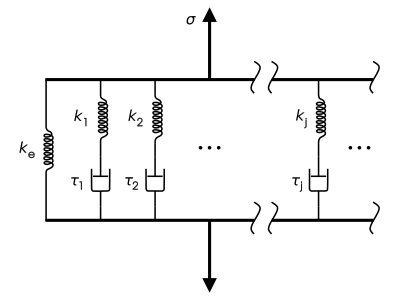
\includegraphics[width=8cm]{images/viscoelasticity/Wiechert.png}\\
{\captionfont From Wikipedia. In this model, several Maxwell elements are assembled in parallel. It takes into account that the relaxation does not occur at a single time, but in a set of times.}
\end{center}



The arrangement shown leads to the following relationships:
\begin{eqnarray}
\dot\varepsilon_{ij}^{\rm mw} &=&  
\underset{\color{teal} 1}{\dot\varepsilon_{ij}^{\rm mw}}  
=\underset{\color{teal}2}{\dot\varepsilon_{ij}^{\rm mw}}  
=\underset{\color{teal} 3}{\dot\varepsilon_{ij}^{\rm mw}}  
=\dots
=\underset{\color{teal} m}{\dot\varepsilon_{ij}^{\rm mw}} \label{eqbob1}
\\
\tau_{ij}^{\rm mw} &=&  \sum_{k=1}^m  \underset{\color{teal}k}{\tau_{ij}^{\rm mw}}
\label{eqbob2}
\end{eqnarray}
Within each row ${\color{teal}k}$ we have the further relationship
\[
\underset{\color{teal}k}{\dot\varepsilon_{ij}^{\rm mw}}  
=\underset{\color{teal} k}{\dot\varepsilon_{ij}^{\rm el}}  
+\underset{\color{teal} k}{\dot\varepsilon_{ij}^{\rm v}}  
\]
\[
\underset{\color{teal} k}{\tau_{ij}^{\rm mw}} 
= \underset{\color{teal} k}{\tau_{ij}^{\rm el}} 
= \underset{\color{teal} k}{\tau_{ij}^{\rm v}}  
\]
and the strain rate is given in terms of 
$\underset{\color{teal} k}{\tau_{ij}^{\rm mw}}$
and stored elastic stress from the previous time step:
\[
\underset{\color{teal}k}{\dot\varepsilon_{ij}^{\rm mw}}
=\left(
\frac{1}{2\; \Delta t_{el} \; G_{\color{teal}k} } 
+ \frac{1}{2 \eta_{\color{teal}k}} 
\right)
\underset{\color{teal} k}{\tau_{ij}^{\rm mw}}
- \frac{1}{2 \Delta t_{el} \; G_{\color{teal}k}  }
\underset{\color{teal} k}{\tau_{ij}}^{\rm mw,0}
\]
Rearranging this expression, we obtain a function for the stress:
\[
\underset{\color{teal} k}{\tau_{ij}^{\rm mw}}
= 2 
\left(
\frac{1}{\Delta t_{el} \; G_{\color{teal}k} } 
+ \frac{1}{\eta_{\color{teal}k}}
\right) ^{-1}
\left(
\underset{\color{teal}k}{\dot\varepsilon_{ij}^{\rm mw}}
+ \frac{1}{2 \Delta t_{el} \; G_{\color{teal}k}  }
\underset{\color{teal} k}{\tau_{ij}}^{\rm mw,0}
\right)
\]
We then define the effective visco-elastic term $\eta^{\rm ve}_{\color{teal}k}$
as follows:
\[
\eta^{\rm ve}_{\color{teal}k}
=
\left(
\frac{1}{\Delta t_{el} \; G_{\color{teal}k} } 
+ \frac{1}{\eta_{\color{teal}k}}
\right) ^{-1}
\]
Then we have 
\[
\underset{\color{teal} k}{\tau_{ij}^{\rm mw}}
= 2 
\eta^{\rm ve}_{\color{teal}k}
\underset{\color{teal}k}{\dot\varepsilon_{ij}^{\rm mw}}
+
\left( \frac{1}{\Delta t_{el} \; G_{\color{teal}k} } 
+ \frac{1}{\eta_{\color{teal}k}} \right) ^{-1}
\frac{1}{ \Delta t_{el} \; G_{\color{teal}k}  } \;
\underset{\color{teal} k}{\tau_{ij}}^{\rm mw,0}
\]
The second term can be simplified:

\begin{eqnarray}
\left( \frac{1}{\Delta t_{el} \; G_{\color{teal}k} } 
+ \frac{1}{\eta_{\color{teal}k}} \right) ^{-1}
\frac{1}{ \Delta t_{el} \; G_{\color{teal}k}  }
&=&
\left( \frac{
\eta_{\color{teal}k} + \Delta t_{el} \; G_{\color{teal}k} 
}{\Delta t_{el} \; G_{\color{teal}k} \eta_{\color{teal}k}} \right) ^{-1}
\frac{1}{ \Delta t_{el} \; G_{\color{teal}k}  } \nn\\
&=&
\frac
{\Delta t_{el} \; G_{\color{teal}k} \eta_{\color{teal}k}} 
{\eta_{\color{teal}k} + \Delta t_{el} \; G_{\color{teal}k} }
\frac{1}{ \Delta t_{el} \; G_{\color{teal}k}  } \nn\\
&=&
\frac{ \eta_{\color{teal}k}} 
{\eta_{\color{teal}k} + \Delta t_{el} \; G_{\color{teal}k} } \nn\\
&=&
\frac{ 1} 
{1 + \Delta t_{el} \; G_{\color{teal}k} /\eta_{\color{teal}k}
} 
\end{eqnarray}
and we now introduce the Maxwell time $t_{{\color{teal}k}}^M = \eta_{{\color{teal}k}} / G_{{\color{teal}k}} $, so that 
we can finally write
\[
\underset{\color{teal} k}{\tau_{ij}^{\rm mw}}
= 2 
\eta^{\rm ve}_{\color{teal}k}
\underset{\color{teal}k}{\dot\varepsilon_{ij}^{\rm mw}}
+
\frac{ 1}{1 + \Delta t_{el} \; / t_{{\color{teal}k}}^M }
\;
\underset{\color{teal} k}{\tau_{ij}}^{\rm mw,0}
\]
By summing of all stresses we obtain the total stress 
(see Eq.~\eqref{eqbob2}):
\[
\tau^{\rm mw}
=\sum_k \underset{\color{teal} k}{\tau_{ij}^{\rm mw}}
=\sum_k
 2 
\eta^{\rm ve}_{\color{teal}k}
\underset{\color{teal}k}{\dot\varepsilon_{ij}^{\rm mw}}
+
\sum_k
\frac{ 1}{1 + \Delta t_{el} \; / t_{{\color{teal}k}}^M }
\;
\underset{\color{teal} k}{\tau_{ij}}^{\rm mw,0}
\]
Using Eq.~\eqref{eqbob1} we can write
\[
\tau^{\rm mw}
= 2 \left(\sum_k  \eta^{\rm ve}_{\color{teal}k} \right)
\dot\varepsilon_{ij}^{\rm mw}
+
\sum_k
\frac{ 1}{1 + \Delta t_{el} \; / t_{{\color{teal}k}}^M }
\;
\underset{\color{teal} k}{\tau_{ij}}^{\rm mw,0}
\]



























\newpage
%==================================================================================================
%==================================================================================================
%==================================================================================================
\section{A remark}

In the absence of gravity, density does not enter the equations. 
As such compressible elasticity is fine. 

If gravitational forces are taken into account, compressible elasticity
means that density should change in space/time. However, 
a lot of the experiments hereafter are written with a constant density, 
meaning that they are reproducible or valid only for incompressible elastic (and viscou) flows!

%==================================================================================================
%==================================================================================================
%==================================================================================================
\section{Analytical Benchmarks}

%..........................................................
\subsection{the 1D solution}
We wish to find the general solution $\tau(t)$ of from the first order ODE
\[
\frac{1}{2\mu} \frac{d\tau}{dt} + \frac{1}{2\eta} \tau = \dot\varepsilon_0
\qquad
\text{or},
\qquad
\frac{d\tau}{dt} + \frac{\mu}{\eta} \tau = 2\mu \dot\varepsilon_0
\]
There is a standard technique to solve such equations, and we start with the following equation instead:
\[
\frac{1}{2\mu} \frac{d\tau}{dt} + \frac{1}{2\eta} \tau = 0
\]
It can be rewritten
\[
\frac{d\tau}{\tau} = -\frac{\mu}{\eta} dt
\]
so
\[
\int \frac{d\tau}{\tau} = -\frac{\mu}{\eta} \int dt
\]
\[
\ln \tau - \ln \tau_0 = -\frac{\mu}{\eta} t 
\]
\[
\ln \tau = -\frac{\mu}{\eta} t  + \ln \tau_0
\]
\[
\tau(t) 
= \exp \left(  -\frac{\mu}{\eta} t  + \ln \tau_0 \right) 
= \exp \left(  -\frac{\mu}{\eta} t   \right)   \exp \left(  \ln \tau_0 \right) 
= \tau_0 \exp \left(  -\frac{\mu}{\eta} t   \right) 
\]
or, using the Maxwell time $t_M=\eta/\mu$,
\[
\tau(t) 
= \tau_0 \exp \left(  -\frac{t}{t_M}   \right) 
\]
Based on this solution we now 
consider the following equation
\begin{eqnarray}
\frac{d}{dt} \left[   \tau \exp\left( \frac{t}{t_M}   \right)  \right]
&=& 
\frac{d \tau}{dt}  \exp\left( \frac{t}{t_M}   \right)  +
\tau \frac{1}{t_M} \exp\left( \frac{t}{t_M}   \right)  \nn\\
&=& 
\left( \underbrace{\frac{d \tau}{dt} + \frac{\mu}{\tau} \tau}_{2\mu \dot\varepsilon_0}  \right)  \exp\left( \frac{t}{t_M}   \right)  \nn
\end{eqnarray}
Then we proceed to integrate both sides:
\[
\int \frac{d}{dt} \left[   \tau \exp\left( \frac{t}{t_M}   \right)  \right] dt
= 2\mu \dot\varepsilon_0 \int \exp\left( \frac{t}{t_M}   \right)  dt
\]

\[
\tau(t) \exp\left( \frac{t}{t_M}   \right)
-
\tau(0) \exp\left( \frac{0}{t_M}   \right)
 =
 2\mu \dot\varepsilon_0  t_M  [ \exp\left( \frac{t}{t_M}   \right)  -  \exp\left( \frac{0}{t_M} \right) ]
\]

\[
\tau(t) \exp\left( \frac{t}{t_M}   \right)
- \tau(0) 
=
2 \mu  \dot\varepsilon_0 \frac{\eta}{\mu} [ \exp\left( \frac{t}{t_M}   \right) -1 ]
\]

\[
\tau(t) \exp\left( \frac{t}{t_M} \right)
=
2 \mu  \dot\varepsilon_0 \frac{\eta}{\mu} [ \exp\left( \frac{t}{t_M}   \right) -1 ] + \tau(0) 
\]

\[
\tau(t) 
=
2 \eta  \dot\varepsilon_0  [1- \exp\left( -\frac{t}{t_M}\right) ] + \tau(0) \exp\left( -\frac{t}{t_M} \right)
\]
which is the solution of Eq.~(4) of \textcite{kabe07} (2007).

\vspace{1cm}
Alternative:

The general solution can be arrived at  
by means of the Laplace transform (?!) and is given by: 
\[
{\bm \tau}(t) = {\bm \tau}(t_0) \exp\left( -\frac{t-t_0}{t_M} \right) + \exp \left(-\frac{t}{t_M}\right)
\int_{t_0}^{t} 2 \mu \dot{\bm \varepsilon}_T  \exp \left(\frac{t'}{t_M}\right) dt'
\]

If $t_0=$ and ${\bm \tau}(t_0)=0$ then
\[
{\bm \tau}(t) =  \exp \left(-\frac{t}{t_M}\right)
\int_{0}^{t} 2 \mu \dot{\bm \varepsilon}_T  \exp \left( \frac{t'}{t_M} \right) dt'
\]
If the strain rate and shear modulus are constant in time, then 
\begin{eqnarray}
{\bm \tau}(t) 
&=&  \exp \left(-\frac{t}{t_M}\right)
2 \mu \dot{\bm \varepsilon}_T   \int_{0}^{t} \exp \left( \frac{t'}{t_M} \right) dt' \nn\\
&=&  \exp \left(-\frac{t}{t_M}\right)
2 \mu \dot{\bm \varepsilon}_T  t_M  \left[ \exp \left( \frac{t}{t_M} \right) -1  \right] \nn\\
&=& 
2 \eta \dot{\bm \varepsilon}_T   \left[ 1 - \exp \left( -\frac{t}{t_M} \right)\right] \nn
\end{eqnarray}
since $t_M=\eta/\mu$.






















%----------------------
\subsection{Pure shear}

{\color{orange} fully incompressible}

The first benchmark performed to test the viscoelastic implementation considers the stress
build-up present in a viscoelastic Maxwell body. Contrary to stressed viscous materials,
viscoelastic materials gradually build-up stress when sheared after which a transition to viscous deformation occurs.

An unstressed, incompressible viscoelastic Maxwell medium is subjected to a velocity field
resulting in pure shear.
The increase of the accumulated stress with time is given by an analytical solution:
\begin{equation}
{\bm \tau} = 2\eta\ {\dot{\bm \varepsilon}} \left ( 1-e^{-\frac{\mu }{\eta} t } \right )
\end{equation}
with $t$ time, $\eta$ the prescribed material viscosity and $\mu$ the prescribed material shear modulus.
The domain size is 100$\times 100$km.
The velocity prescribed at all boundaries equals $v=1$ cm/yr in magnitude yielding a constant
background strain rate of $\dot{\varepsilon}=2\text{cm/yr}/100\text{km}\simeq \SI{6.342e-15}{\per\second}$.
The viscosity is $\eta= 10^{21}\text{Pa.s}$, the shear modulus is
$\mu =10^{10}$Pa and the gravity is set to zero. We set $\delta t=100$yr.

\begin{center}
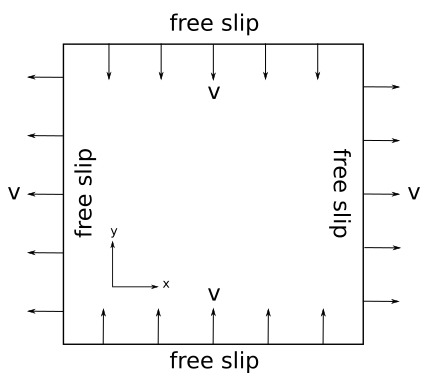
\includegraphics[width=5cm]{images/viscoelasticity/stress_buildup_setup.png}\\
\captionfont{Set up of the stress build-up benchmark. All domain sides have a free slip
boundary condition, and pure shear velocity conditions are prescribed. Adapted from
Gerya (2010) \cite{gery10}.}
\end{center}

We have
\[
\eta_{eff} 
= \frac{\eta \delta t}{\delta t + \eta/\mu} 
= \frac{10^{21} \cdot 3.154\times 10^{9}}{3.154\times 10^{9} + 10^{21}/10^{10}} 
\simeq 
3.0592 \times 10^{19}\text{Pa.s}
\qquad
\text{and}
\qquad
Z=\frac{\eta_{eff}}{\mu \delta t} 
\simeq 
0.9694
\]
The Maxwell time is $t_M = \frac{\eta}{\mu} = 10^{11}\text{s} \simeq 3171\text{yr}$.
In the absence of elasticity (purely viscous behaviour), we have
$\dot{\varepsilon}_{xx} = 6.342\times 10^{-15}$
and $\eta=10^{21}$ so the
deviatoric stress $\tau_{xx}$ is equal to
\[
\tau_{xx} = 2 \cdot 10^{21} \cdot 6.342\times 10^{-15} \simeq 12.68 \times 10^6 \text{Pa}
\]

The first time that the Stokes system is solved, there is no stored stress, i.e. the
elastic rhs is identically zero, so that the system is solved with a viscosity equal to
$\eta_{eff}$.
We can easily compute the analytical solution, and we see that $\dot{\varepsilon}_{xy}=0$
and $\dot{\omega}_{xy}=0$, which we recover:

Results in Stone 64!

%\begin{center}
%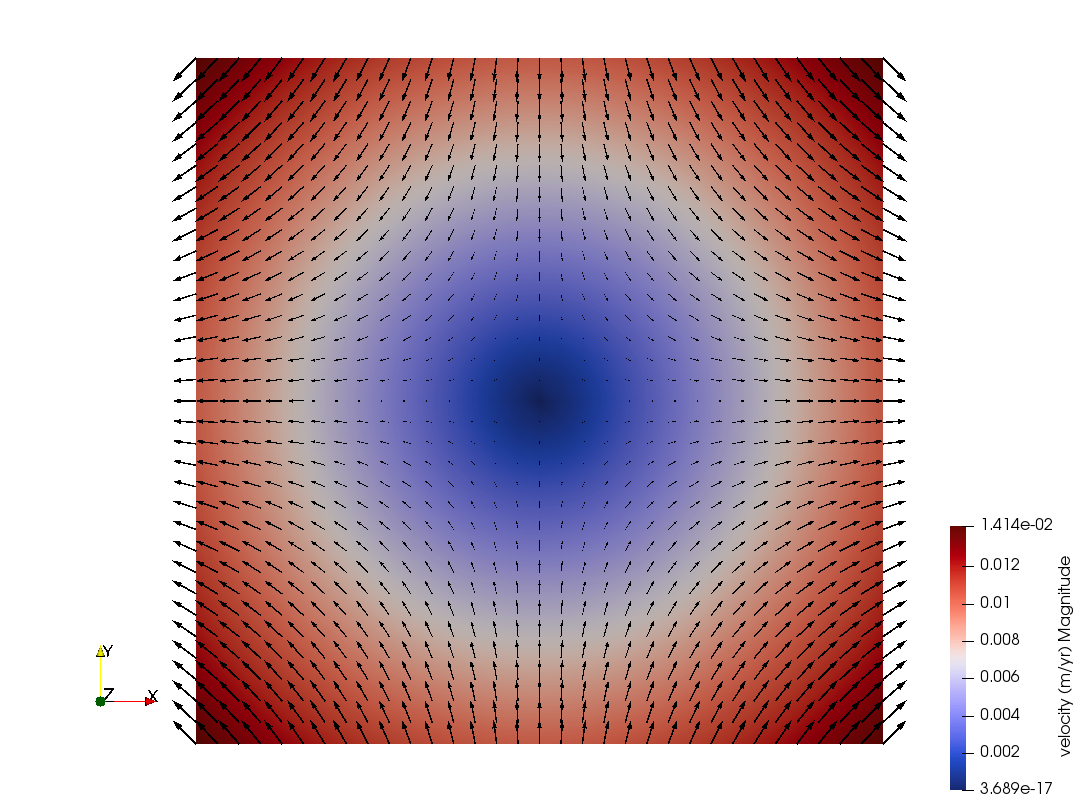
\includegraphics[width=5cm]{python_codes/fieldstone_64/results/buildup_11/init/vel}
%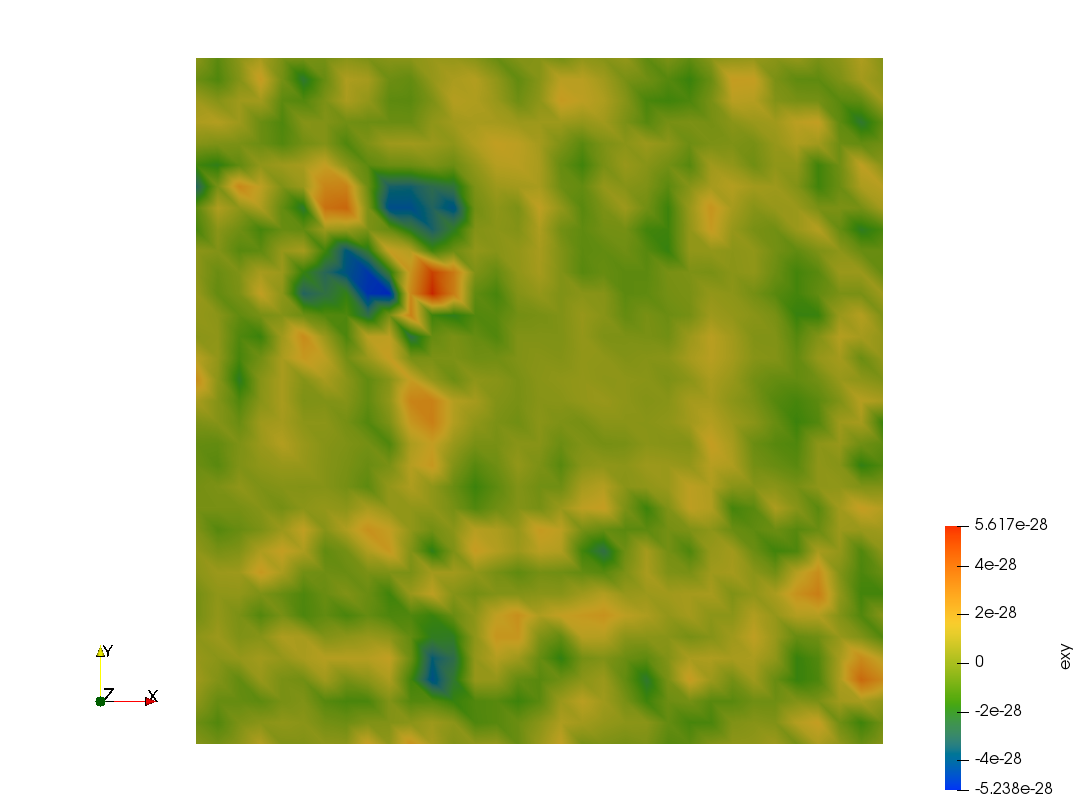
\includegraphics[width=5cm]{python_codes/fieldstone_64/results/buildup_11/init/exy}
%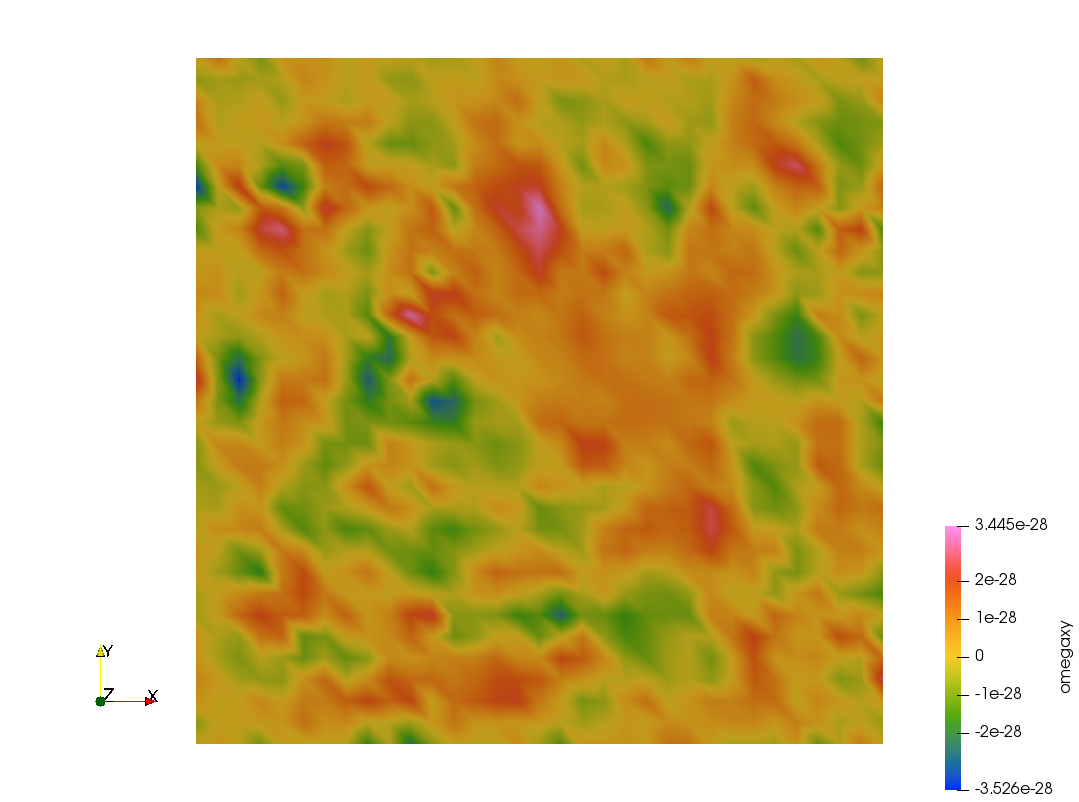
\includegraphics[width=5cm]{python_codes/fieldstone_64/results/buildup_11/init/oxy}
%\end{center}

The expected stress value for $\tau_{xx}$ after the first Stokes solve is
\[
\tau_{xx} = 2 \eta_{eff} \dot{\varepsilon}_{xx} 
= 2 \cdot 3.057\times 10^{19} \cdot 6.342\times 10^{-15} 
\simeq 38.775 \times 10^4 \text{Pa}
\]

Also check Gerya's book page 358 2nd edition ?


%-----------------------------------------------------------
\subsection{Simple shear (Muhlhaus \& Regenauer-Lieb, 2005)}

\fullcite{mure05}

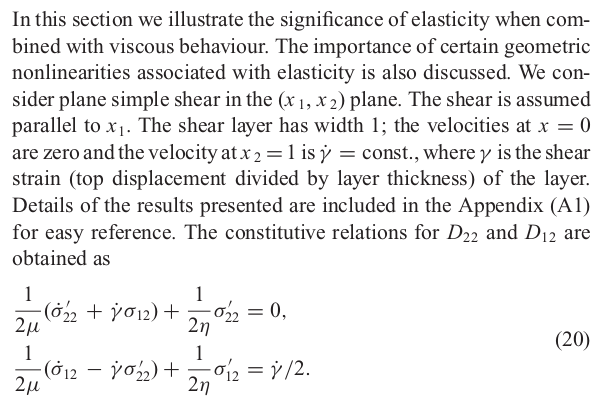
\includegraphics[width=7cm]{images/viscoelasticity/mure05_ss1}
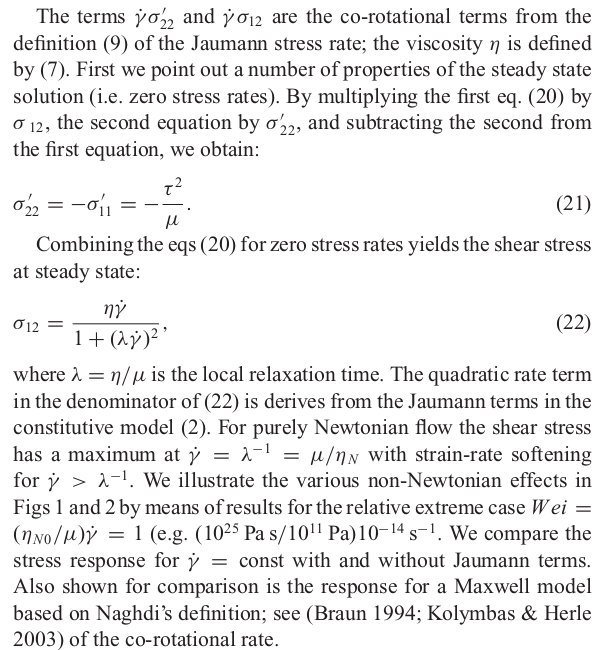
\includegraphics[width=7cm]{images/viscoelasticity/mure05_ss2}
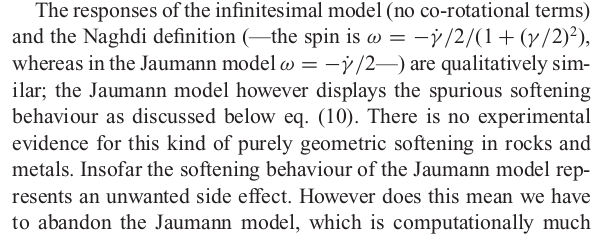
\includegraphics[width=7cm]{images/viscoelasticity/mure05_ss3}
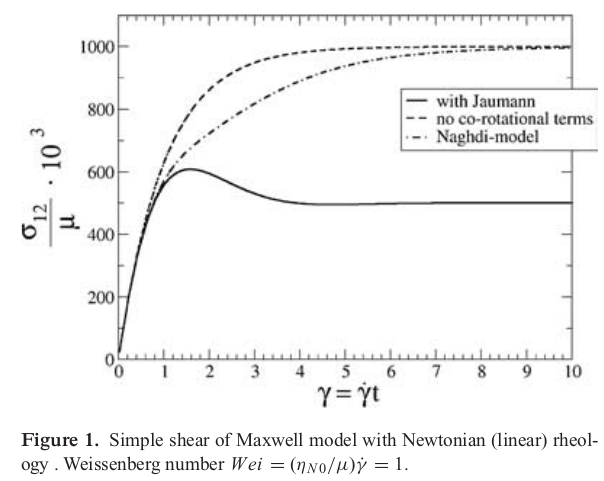
\includegraphics[width=7cm]{images/viscoelasticity/mure05_ss4}
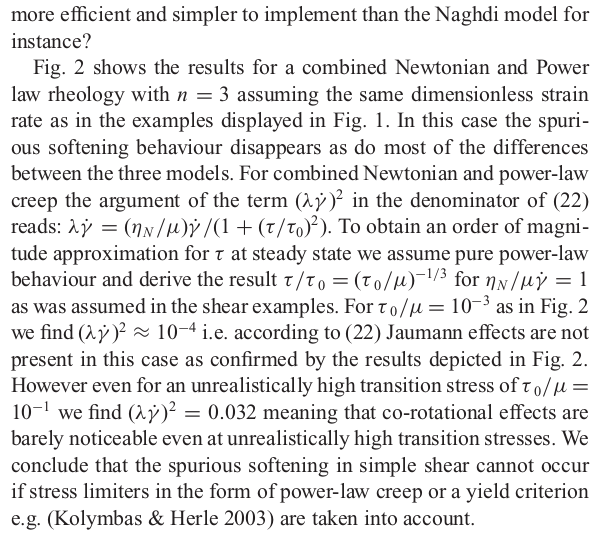
\includegraphics[width=7cm]{images/viscoelasticity/mure05_ss5}
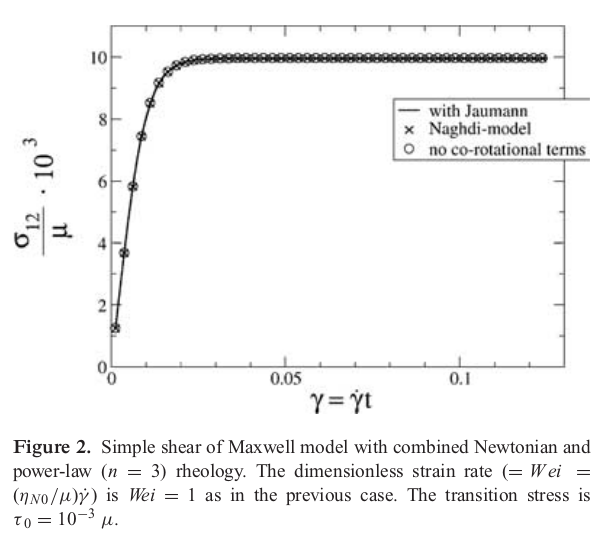
\includegraphics[width=7cm]{images/viscoelasticity/mure05_ss6}


%---------------------------------------------------------------------
\subsection{Simple Shear (von Tscharner and Schmalholz, 2015)}

\fullcite{vosc15}

This experiment uses a homogeneous cube with the dimensions 1x1x1 which is
deformed by simple shear. The bottom boundary is fixed 
(i.e., the boundary condition is no slip), the
velocities on the top surface are prescribed in x-direction to generate 
simple shear and the top boundary is fixed in z-direction. 
The boundary conditions are free slip for two vertical boundaries (y=0 and
y=1) and the two remaining vertical boundaries (x=0 and x=1) are free. 
The viscosity and the elastic shear modulus are $\eta=10^{10}$ and $G=1$, 
respectively. All model dimensions and material parameters
are given in dimensionless numbers using the model length, the elastic 
shear modulus and the background strain rate as characteristic parameters. 
The results for two simulations, one with Jaumann correction and one without 
Jaumann correction, are given in Figure B5 where the colors indicate the
second invariant of the stress tensor. The results with the Jaumann correction 
show a homogeneous distribution of stress (Figures a–d), whereas the distribution 
of the second invariant of the stress tensor is inhomogeneous without the 
Jaumann correction and the simulation ‘‘crashes’’ for high strain
(Figures e–h).

\begin{center}
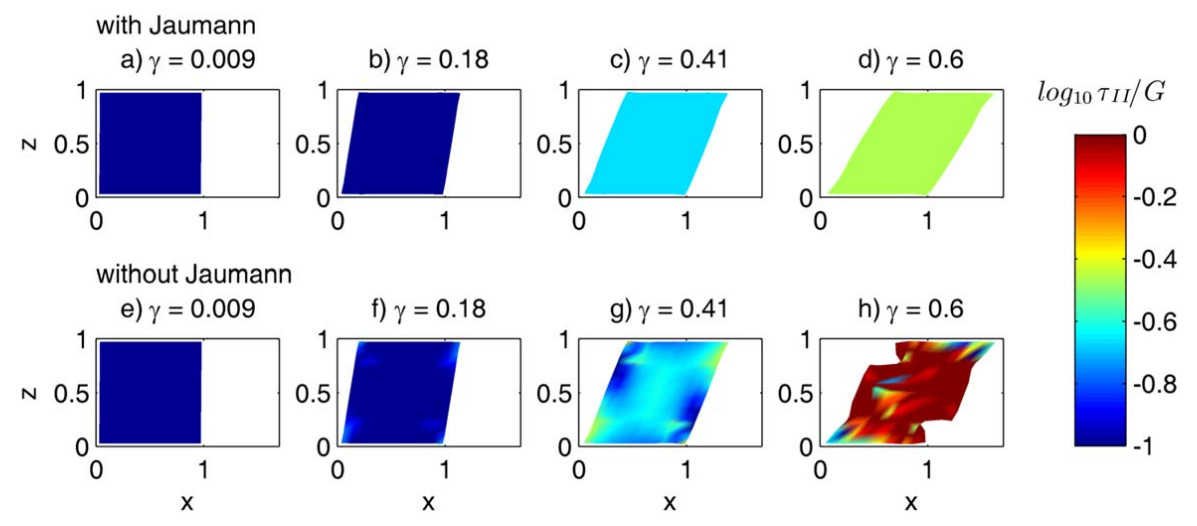
\includegraphics[width=15cm]{images/viscoelasticity/vosc15b}\\
{\captionfont Deformation of a homogeneous cube under simple shear (a–d) with 
Jaumann correction and (e–h) without Jaumann correction for different amounts of bulk shear strain c
(i.e., ratio of maximal horizontal displacement to model thickness). The colors indicate 
the second invariant of the stress tensor $\tau_{ii}$. Without the Jaumann corrections, the stress 
distribution becomes inhomogeneous and the simulation crashes for high strain.}
\end{center}


%----------------------------------------
\subsection{Rayleigh-Taylor instability}

{\color{orange} fully incompressible}

This experiment is presented in \textcite{kabe07} (2007).

The model consists of a viscoelastic layer of thickness $H_1$ , with density $\rho_1$, 
viscosity $\eta_1$ and elastic shear module $\mu_1$ that overlies a viscous
layer of thickness $H-H_1$ , with density $\rho_2$ and viscosity $\mu_2$. 
The interface between the two fluids is perturbed sinusoidally according
to $h(x) = (H - H_1 ) + A_0 \cos (2\pi x/ \lambda )$, 
where $H_1$ is the thickness of the upper layer, $H$ the height of the model, 
$A_0$ the initial amplitude and $\lambda$ the wavelength of the perturbation. 
If $\rho_1>\rho_2$, the system is gravitationally unstable.

\begin{center}
\fbox{
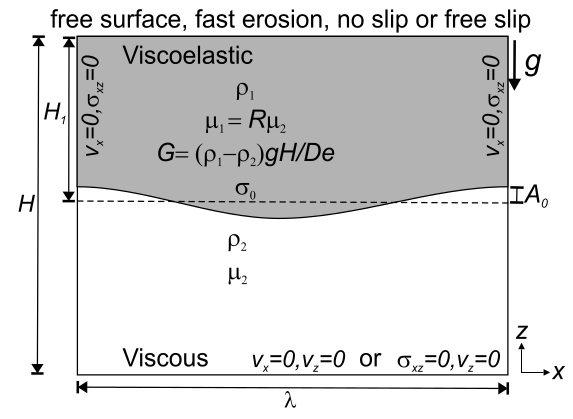
\includegraphics[width=12cm]{images/viscoelasticity/kabe07}}\\
{\captionfont Taken from \textcite{kabe07}.}
\end{center}

The Deborah number is given by
\[
De=\frac{(\rho_1-\rho_2)g H}{\mu}
\]
and is here defined as the ratio between the viscous (Stokes) timescale ($(\rho_1-\rho_2)g H/\eta_1$)
and the viscoelastic timescale $\eta_1/\mu$ of the upper layer.
The authors state: ``
Interestingly, the Deborah number, which is a measure of the importance of
elasticity [...], is independent on the viscosity of the system. 
This is due to the fact that the magnitude of stress is solely
dependent on the density difference for purely buoyancy-driven flow.''
Also: ``
In the present definition of the Deborah number realistic values for 
lithospheric-scale deformation are $10^{-4} \le De \le 1$ 
(with $\rho =10-330~\si{\kg\per\cubic\meter}$ , 
$g = 10~\si{\meter\per\square\second}$ , $H = 100-3000~\si{\km}$, 
$\mu=10^{10}-10^{11}~\si{\pascal}$).''

Another parameter controlling the dynamics of the system is the viscosity contrast 
between the upper and the lower layer, expressed by $R=\eta_1/\eta_2$.

We here set $H=500~\si{\km}$, $H_1=100~\si{\km}$,
$\rho_2=3300~\si{\kg\per\cubic\meter}$, $\eta_2=10^{21}~\si{\pascal\second}$,
$\mu_1=\mu_2=10^{10}~\si{\pascal}$, $\eta_1=R\eta_2$,
$A_0=1~\si{\km}$, $\lambda=L_x$.







%..........................................................
\subsection{stress build-up inside an elastic inclusion in a viscous matrix (Beuchert \& Podlachikov, 2010)}

This is presented in Section 5.4 of \fullcite{bepo10}

{\color{orange} fully incompressible}

The authors test their viscoelastic FEM model against the analytical solution 
for stress built-up inside an elastic inclusion in a viscous matrix under pure shear. 

\todo[inline]{include figure - not in paper}

Note that the fluid in question is incompressible as shown by their Eq.~(3).

An analytical solution applicable for the time-dependent stress evolution inside 
a viscoelastic inclusion embedded in a viscous matrix can be derived:
\[
\tau_{xx} = -\frac{(a+1)^2 \left[-1+\exp -\frac{2\mu a t }{a^2+1}  \right]}{a} \dot\varepsilon^d_{xx}
\]
where $a$ is the aspect ratio of the inclusion and the matrix viscosity is assumed to be unity.

For this equation to be applicable to our viscoelastic model, we prescribe a
high viscosity inside the inclusion ($\eta_{inclusion}=10^5$) and thus obtain an 
elastic response inside the inclusion. For the matrix, we apply a viscous
rheology with viscosity $\eta_{matrix} =1$.

\begin{center}
\fbox{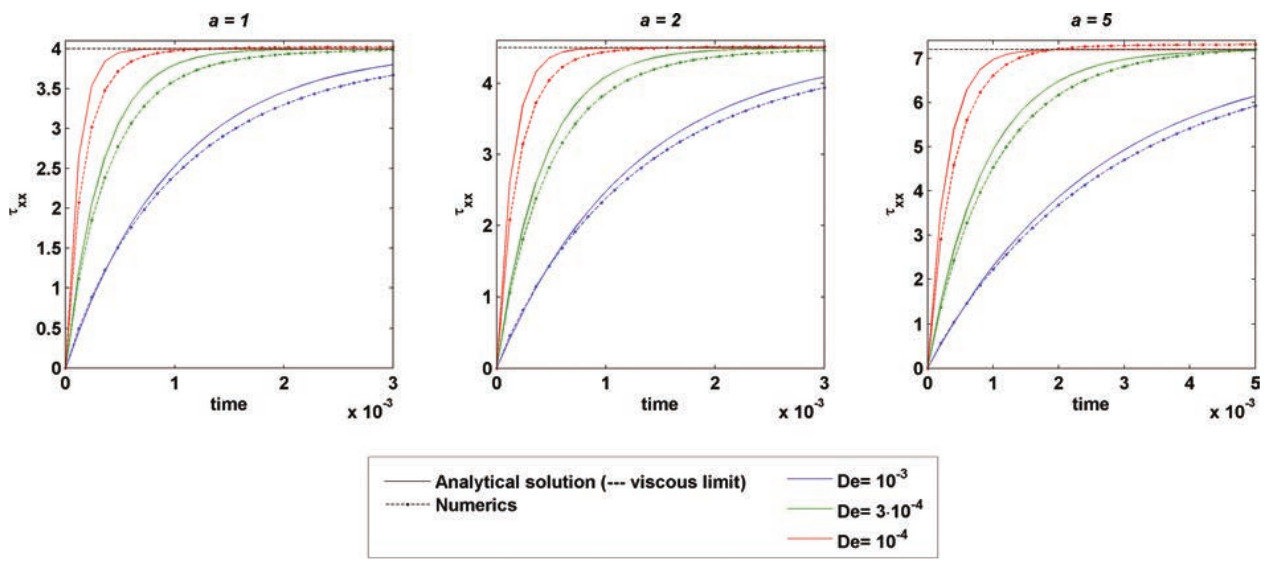
\includegraphics[width=17cm]{images/viscoelasticity/bepo10}}\\
{\captionfont Taken from \textcite{bepo10}.
Stress built-up inside an elliptical elastic inclusion with aspect ratios 
$a =1,2,5$ embedded in a viscous matrix under constant pure shear
loading. Comparison of the analytical solution 
with the numerical solution obtained in their FEM model for different values 
of Deborah number $De = 10^{-4},3\cdot10^{-4},10^{-3}$ 
at non-dimensional deviatoric strain rate $\dot\varepsilon_{xx}^d=1$. 
Time and deviatoric stress $\tau_{xx}$are non-dimensional.
The test results show a good agreement of the numerical solution with the 
analytical solution. For time $t\rightarrow \infty$, the solution for
stress inside the elastic inclusion converges towards the solution for stress 
inside a viscous inclusion (dashed horizontal line ‘viscous limit’).
}
\end{center}


%------------------------------------------------------------------------------------------
\subsection{Viscoelastic flow past a cylinder in a channel (Beuchert \& Podlachikov, 2010)}

\fullcite{bepo10}

This is presented in Section 5.4 of \textcite{bepo10} (2010).

We tested the flow code against a numerical benchmark for iso-viscous, 
viscoelastic flow past a circular cylinder in a channel. Figure below shows
the domain setup and boundary conditions for this benchmark. The radius of the circular 
cylinder $r=1$ is half the domain height and the
domain aspect ratio is $3:1$. 


\begin{center}
\fbox{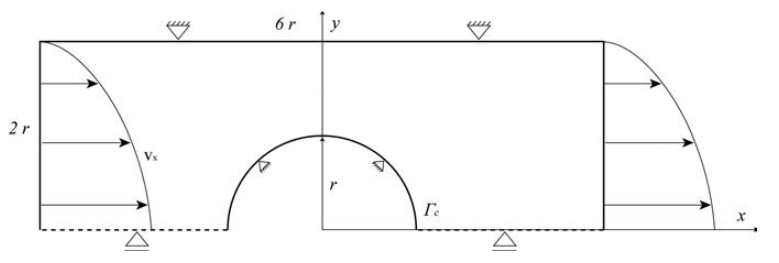
\includegraphics[width=17cm]{images/viscoelasticity/bepo10a}}\\
{\captionfont Taken from \textcite{bepo10}.
Setup for the benchmark of viscous flow past circular cylinder in a channel. 
The domain is symmetric about the horizontal axis and thus only the
upper half of the channel is modelled.
}
\end{center}


At the inflow and outflow boundaries, an established Poiseuille flow 
$v_x = 3(R^2 -y^2 )/(2R^2)$ is imposed; $v_y=0$ at
the sides. Both upper and lower boundaries are fixed in $y$-direction. We apply no-slip boundary conditions at the top and along the cylinder
wall and free-slip (zero traction) conditions at the bottom (symmetry axis). For the inflow conditions on $\sigma$ , we use the analytical solution for
simple shear of a Jaumann fluid, which is valid for Poiseuille flow. In that case, the Jaumann derivative equations are
\begin{eqnarray}
\tau_{xx}+2 De \omega \tau_{xy} &=& 0 \\
\tau_{yy}+2 De \omega \tau_{xy} &=& 0 \\
\tau_{xy}+2 De \omega (\tau_{yy}-\tau_{xx}) &=& 2 \mu \dot{\varepsilon}_{xy} \\
\end{eqnarray}
Given that $\dot\gamma = 2\dot\varepsilon_{xy}$ and $\omega = -1/2 \dot\gamma$ for simple shear, we obtain from the equation above
\[
\tau_{xy} = \frac{2 \mu \dot\varepsilon_{xy}}{1+4De^2\omega^2}
= \frac{\mu \dot\gamma}{1+4De^2\omega^2}
=\frac{\mu \dot\gamma}{1+2 De^2 \dot{\gamma}^2}
\]
and can then solve for $\tau_{xx}$ and $\tau_{yy}$ by substitution.
The strain rate $\dot\gamma$ is given by $\partial v_x /\partial y$, 
that is, by differentiating the inflow
condition $v_x = 3(R^2 -y^2 )/(2R^2)$ 
with respect to $y$, resulting in $\dot\gamma= -3y/R^2$ at the inflow boundary.

The authors further measure the non-dimensional drag force $C_d$ exerted by the passing fluid on the cylinder wall and compare it with published values.



\begin{center}
\fbox{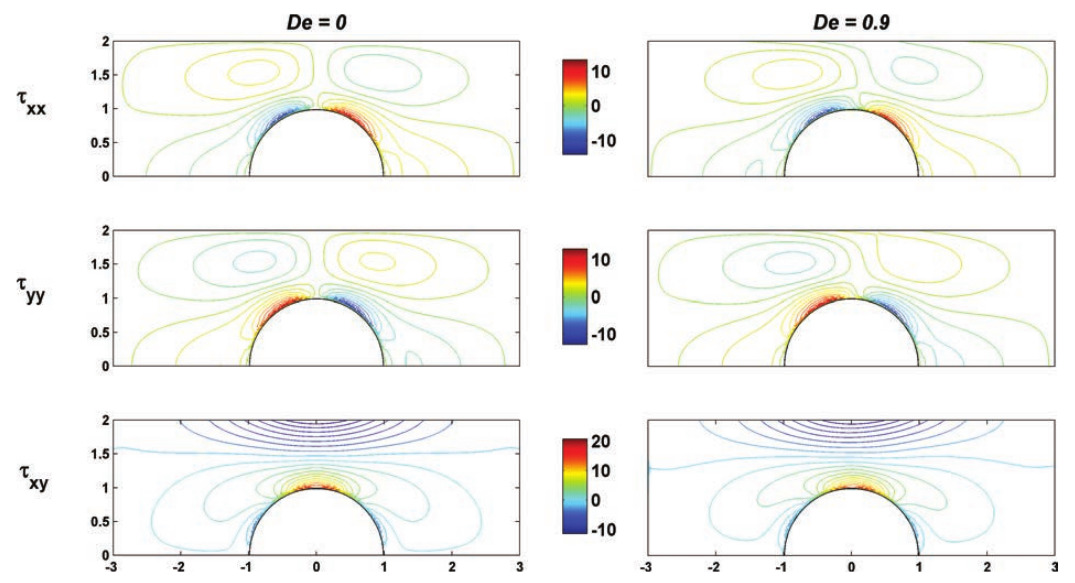
\includegraphics[width=17cm]{images/viscoelasticity/bepo10b}}\\
{\captionfont Taken from \textcite{bepo10}.
Non-dimensional deviatoric stresses $\tau$ at $De = 0$ and $De = 0.9$ 
resulting from fluid flow past a cylinder in a channel. The benchmark is conducted
on a regular, structured grid at resolution $600 \times 200$ nodes.
}
\end{center}

%------------------------------------------------------------------------------------------
\subsection{Flow around rigid circular cylinders (Muhlhaus and Regenauer-Lieb, 2005)}


\fullcite{mure05}

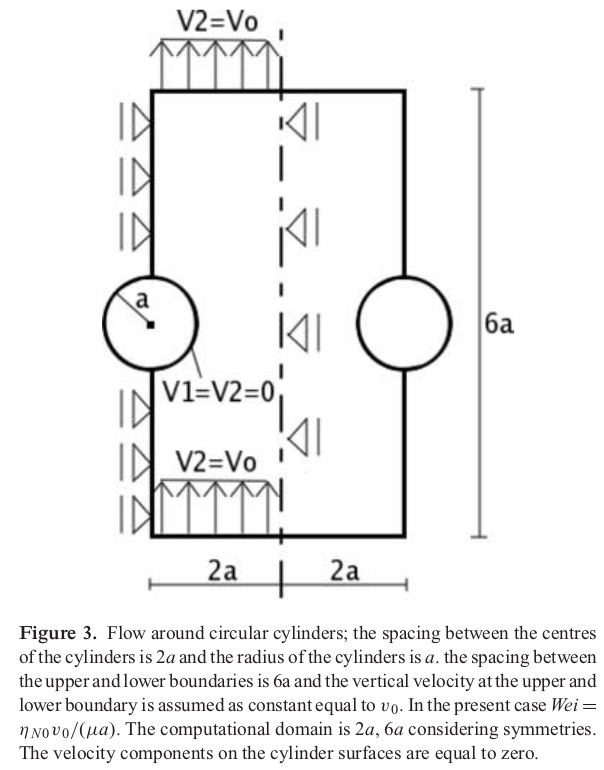
\includegraphics[width=7cm]{images/viscoelasticity/mure05_cyl1}
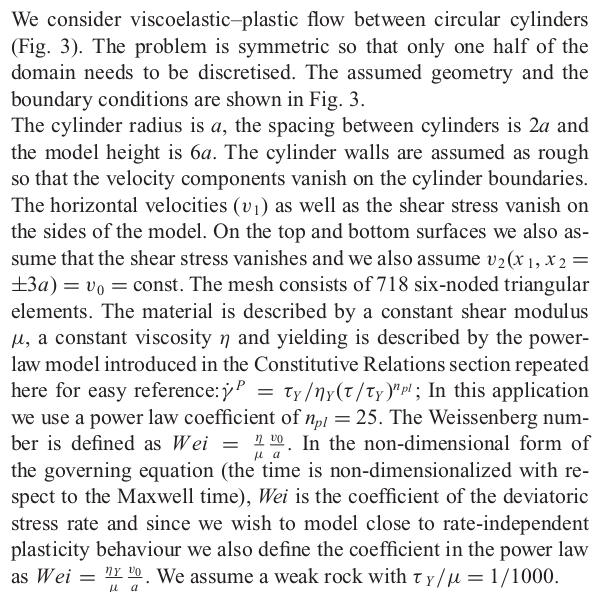
\includegraphics[width=7cm]{images/viscoelasticity/mure05_cyl2}
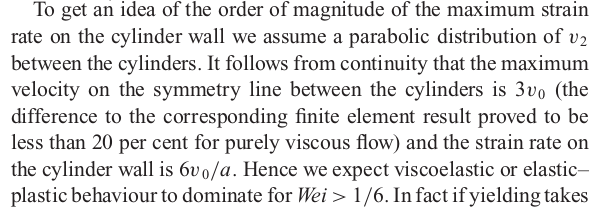
\includegraphics[width=7cm]{images/viscoelasticity/mure05_cyl3}
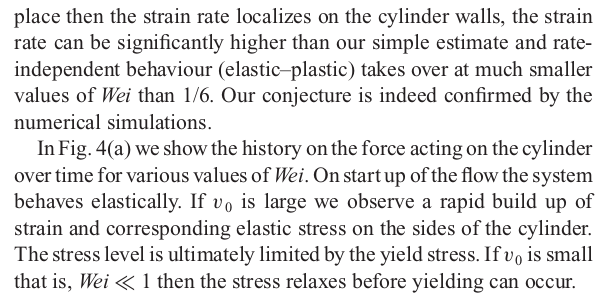
\includegraphics[width=7cm]{images/viscoelasticity/mure05_cyl4}
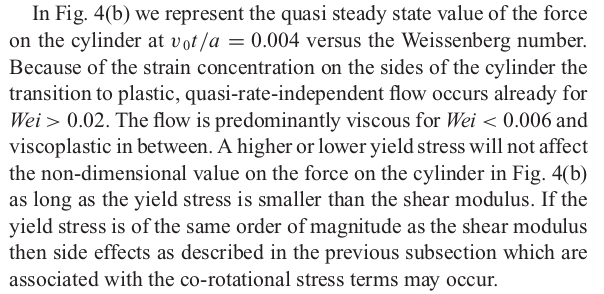
\includegraphics[width=7cm]{images/viscoelasticity/mure05_cyl5}
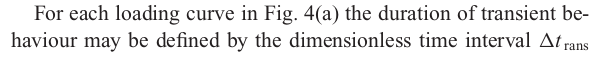
\includegraphics[width=7cm]{images/viscoelasticity/mure05_cyl6}
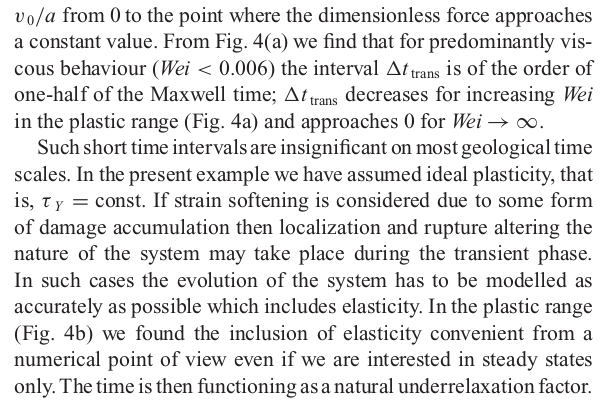
\includegraphics[width=7cm]{images/viscoelasticity/mure05_cyl7}
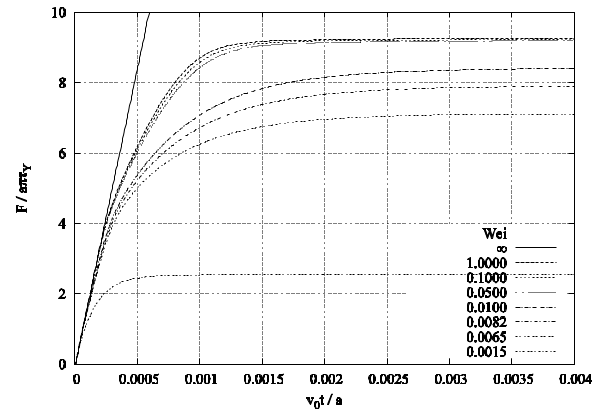
\includegraphics[width=7cm]{images/viscoelasticity/mure05_cyl8}
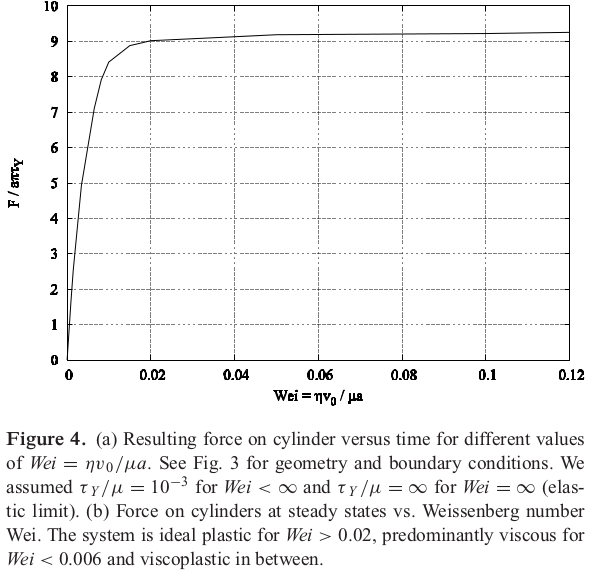
\includegraphics[width=7cm]{images/viscoelasticity/mure05_cyl9}














%---------------------------------------------------------------------------
\subsection{Response to load from ice sheet (Nakiboglu and Lambeck, 1982)}

\fullcite{nala82}

The domain is $500\times500$km. Vertical gravity is 9.8, density is 3300, viscosity 
is $3\cdot10^{20}~\si{\pascal\second}$, 
shear modulus is $10^{10}~\si{\pascal}$, free slip on left, right and bottom. 
A normal stress is imposed on the top for $0<x<100$km. It corresponds to  
an ice sheet of density $\rho_i=900$ of 1000m height. 
The timestep is set to 100yr. Resolution is set to $50\times50$ elements.
Stress/traction b.c. are explained in Section~\ref{ss:openbc}.

Analytical solution is provided in Nakiboglu and Lambeck (1982) \cite{nala82}. 
Note however that this is a 2D setup while the original solution is for a 
cylindrical load and also for a semi-infinite domain.

Effective viscosity is given by
\[
\eta_{eff} = \frac{\eta \delta t}{\delta t + \eta/\mu}
= 2.85362675546547e+19
\]

\begin{center}
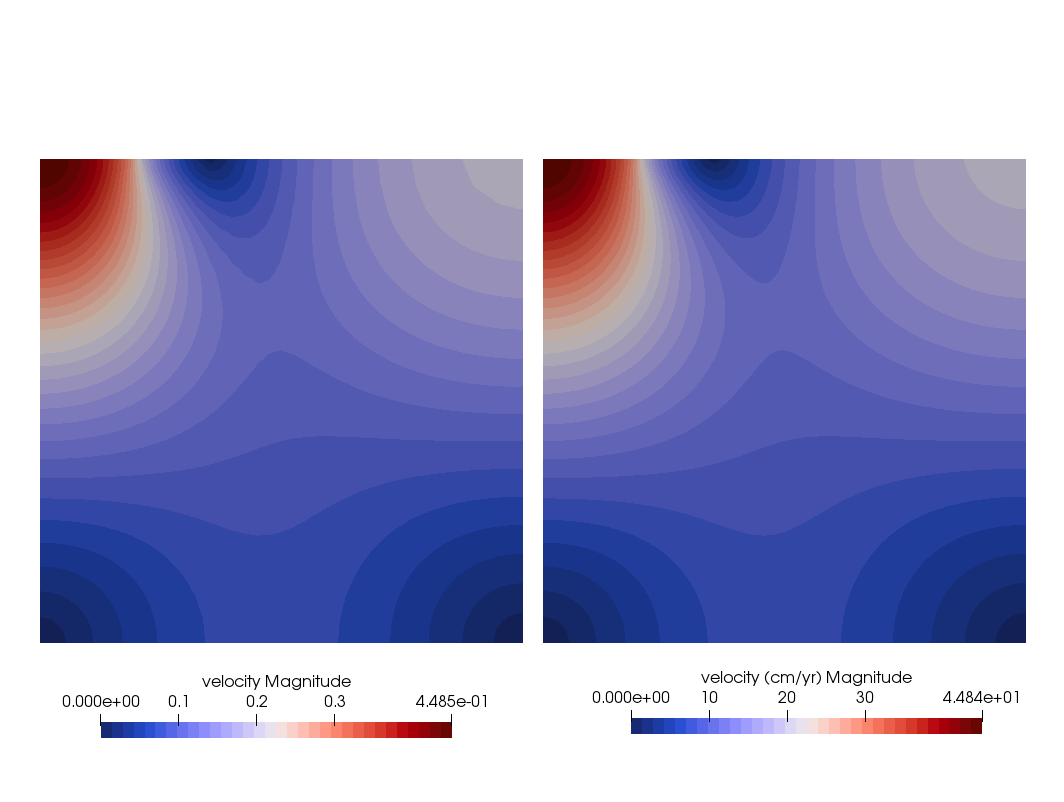
\includegraphics[width=10cm]{python_codes/fieldstone_64/results/icesheetload/vel}\\
{\captionfont Left: ASPECT; Right: stone 64} 
\end{center}


It was run with ASPECT: prm file in stone 64 results folder.


%--------------------------------------------------------------------------------------------
\subsection{Rectangular sample of material under a constant downward velocity applied on top}

\fullcite{modm01}

\begin{center}
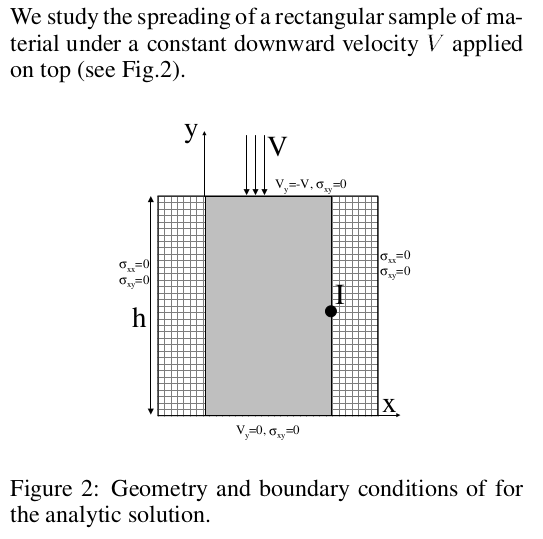
\includegraphics[width=8cm]{images/viscoelasticity/bench_modm01a}
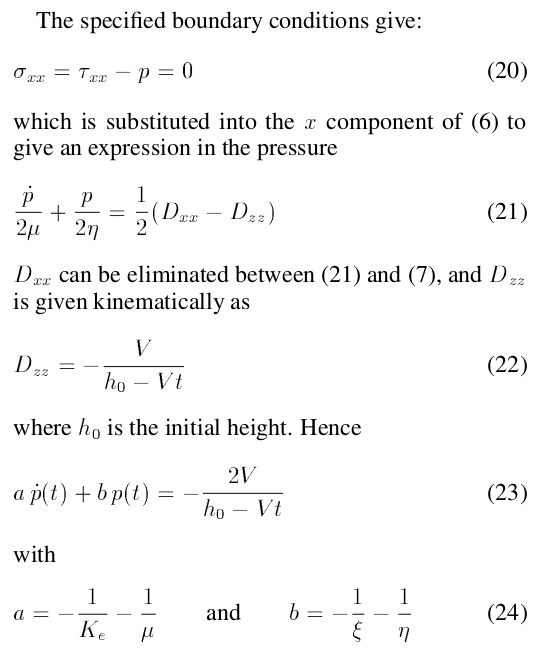
\includegraphics[width=8cm]{images/viscoelasticity/bench_modm01b}\\
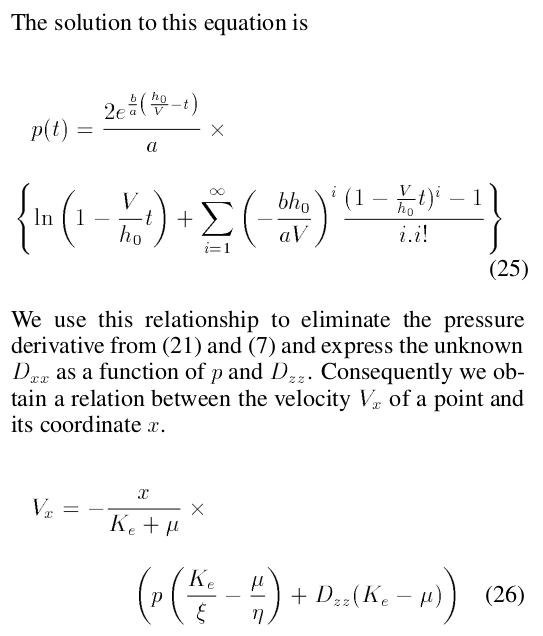
\includegraphics[width=8cm]{images/viscoelasticity/bench_modm01c}
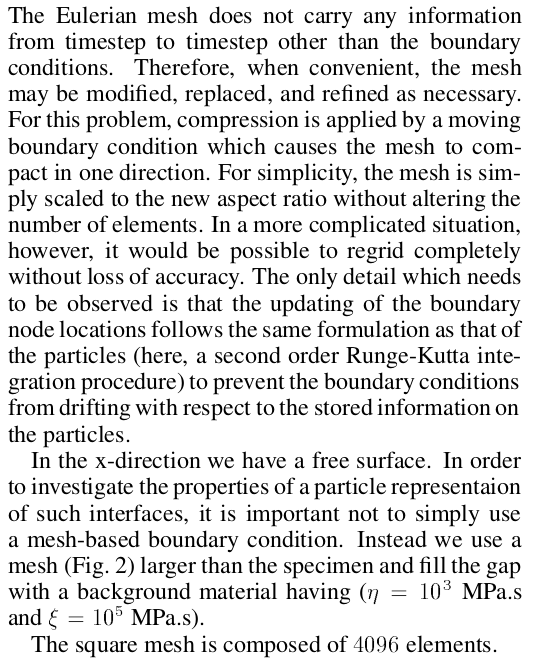
\includegraphics[width=8cm]{images/viscoelasticity/bench_modm01d}\\
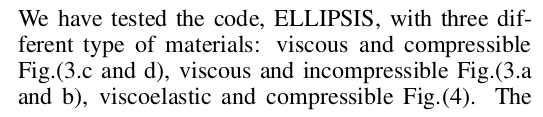
\includegraphics[width=8cm]{images/viscoelasticity/bench_modm01e}
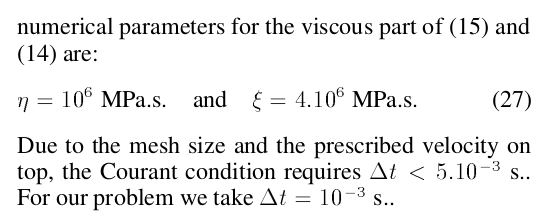
\includegraphics[width=8cm]{images/viscoelasticity/bench_modm01f}\\
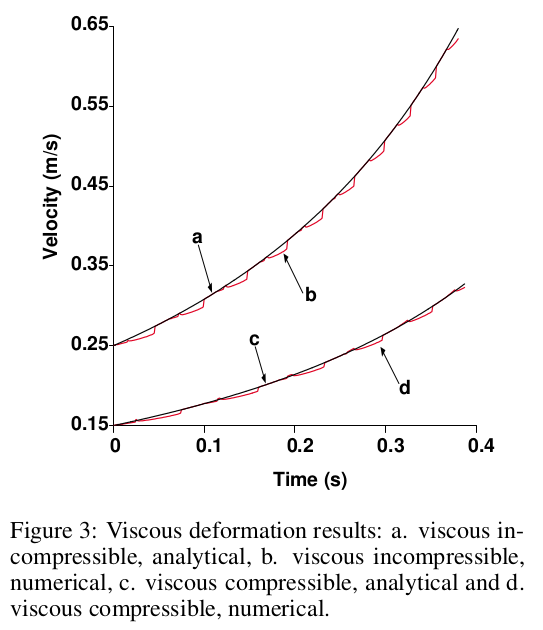
\includegraphics[width=8cm]{images/viscoelasticity/bench_modm01g}
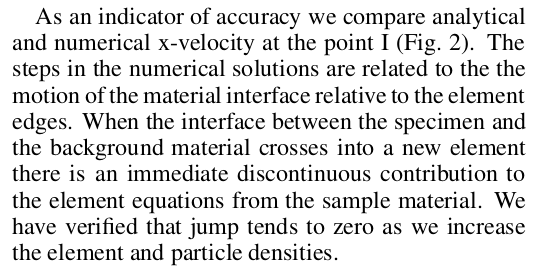
\includegraphics[width=8cm]{images/viscoelasticity/bench_modm01h}\\
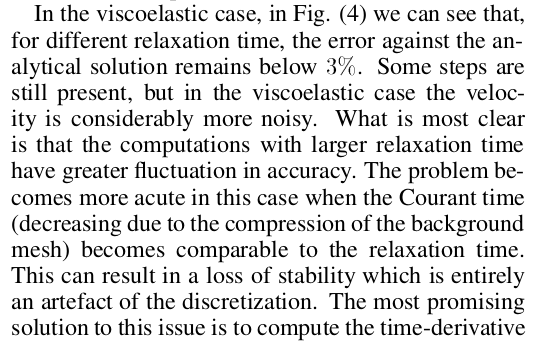
\includegraphics[width=8cm]{images/viscoelasticity/bench_modm01i}
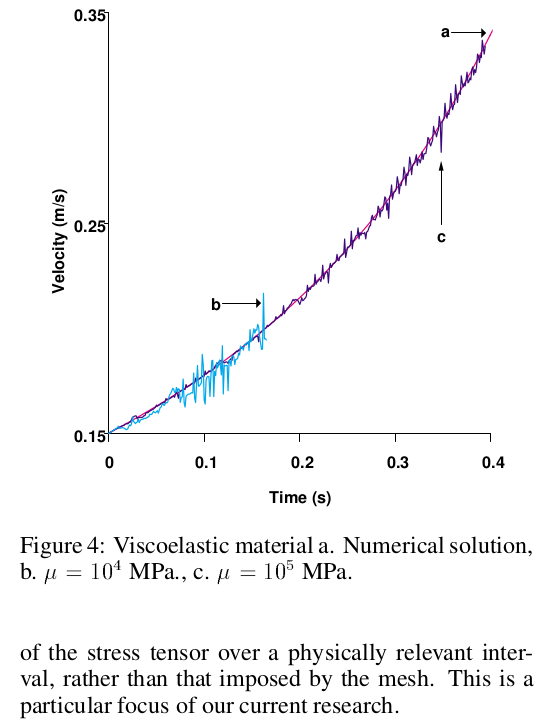
\includegraphics[width=8cm]{images/viscoelasticity/bench_modm01j}\\
\end{center}



%--------------------------------------------------------------------------------------------
\subsection{pressure field evolution during folding of viscoelastic multilayers (Schmalholz et al, 2001)}

\fullcite{scps01}

The deformation of the heterogeneous, viscoelastic material is
simulated in two dimensions for plane strain, incompressible
materials and in the absence of gravity. 

\begin{center}
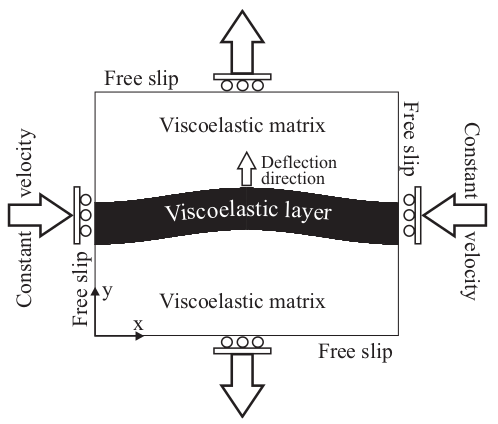
\includegraphics[width=8cm]{images/viscoelasticity/scps01a}
\end{center}








%==================================================================================================
%==================================================================================================
%==================================================================================================
\section{Numerical Benchmarks/Experiments}

%--------------------------------------------------
\subsection{Bending of elastic slab (Gerya's book)}

The sinking slab benchmark consists of a beam of elastic material which is placed 
in a weak and viscous surrounding medium. The initially unstressed beam is attached to the left 
domain boundary through boundary conditions. A stress is then applied to the beam in the form of 
gravity. The applied gravity force results in the deformation of the beam through bending. 
After 20 kyr, the gravity field is turned off and the elastic properties of the beam will then 
force itself to its original position. The set-up of the benchmark is given in the following figure:

\begin{center}
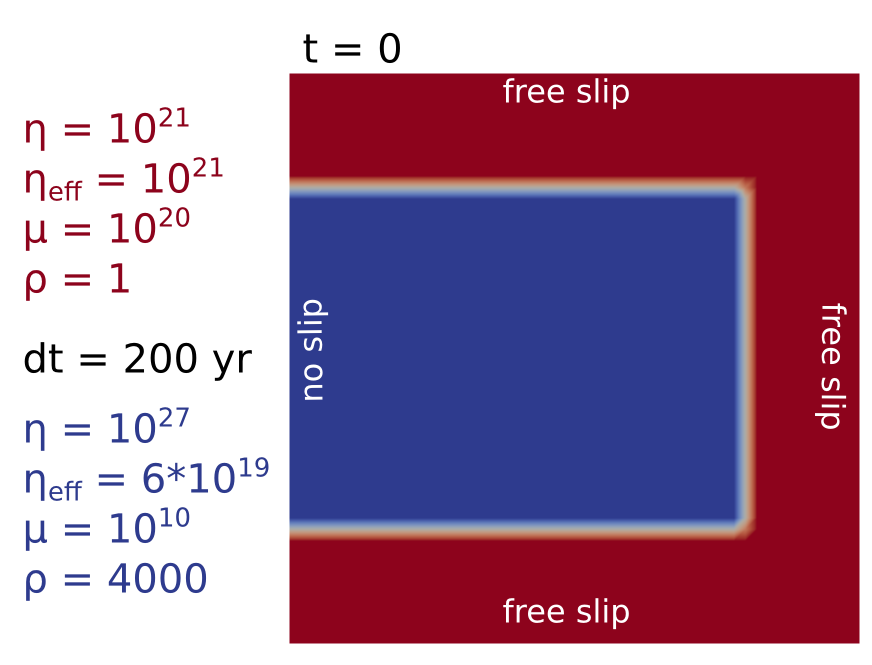
\includegraphics[width=6cm]{images/viscoelasticity/poster_benchmark.png}\\
\captionfont{Set-up of the benchmark from \cite{gery10}. The properties of the
two materials are given on the left, together\\ with the initial configuration of the benchmark.}
\end{center}

The beam is surrounded by a low-density, low-viscosity and high shear modulus medium
of which the specifications are given in  the following table.
The boundary conditions of the domain consist of a no slip condition at
the left boundary where the slab is attached and free slip boundary conditions along all other sides.
The results are calculated on a grid with a resolution of 50x50 elements containing 64 randomly 
distributed markers at startup.
The time step is set to $\delta t = 200yr$ (i.e. gravity is switched off after 100 time steps).

\begin{center}
\begin{tabular}{lll}
\hline
\textit{Material properties}& \textit{Elastic slab (fluid 1)}  & \textit{Surrounding medium (fluid 2)} \\
\hline
\hline
Density         $\rho$ \     [kg/m$^{3}$]      & 4000                    & 1     \\
Viscosity       $\eta$ \    [Pa$\cdot$ s]      & $10^{27}$               &   $10^{21}$     \\
Shear modulus   $\mu $ \    [Pa]               & $10^{10}$               & $10^{20}$       \\
Maxwell time $t_M$     \    [yr]               & 3.17Gyr                 &  $3.17\times10^{-7}$yr       \\
eff. visc.      $\eta_{eff}$ \ [Pa$\cdot$s]    & 6.307199602192306e+19   &  9.999999984145105e+20      \\
visco-elasticity factor $Z$      \ [-]         & 0.9999999369280039      &  1.5854895966744522e-09     \\
\hline
\end{tabular}
\end{center}








%--------------------------------------------------------------------------
\subsection{Flexure of elastic plate (Choi et al, 2013) \label{sec:chtl13}}


This benchmark is presented in \textcite{chtl13} (2013). 
The setup is as follows:

\begin{center}
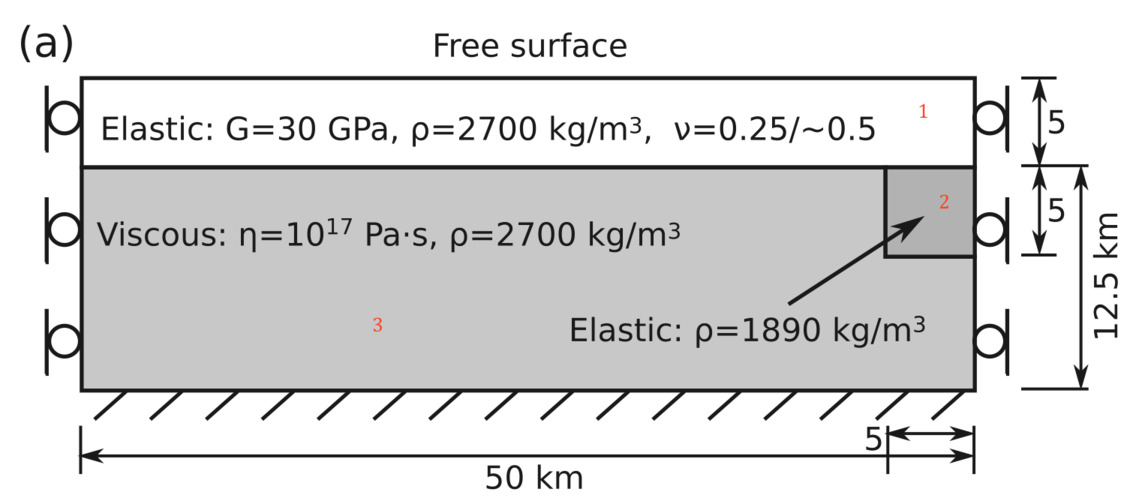
\includegraphics[width=9cm]{images/viscoelasticity/chtl13a}
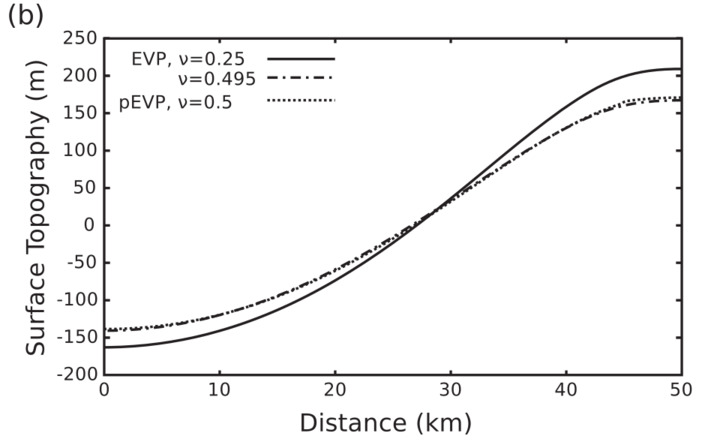
\includegraphics[width=7cm]{images/viscoelasticity/chtl13b}\\
{\captionfont 
Taken from \textcite{chtl13}. ``Effect of elastic compressibility on the prediction 
of an elastic thin plate subject to an uplifting load. (a)
Model setup for a finite length elastic layer subjected to a
finite length buoyant load applied on the bottom. (b) Profiles
of mean-subtracted surface topography.''}
\end{center}

\begin{center}
\begin{tabular}{llll}
\hline 
\textit{Material properties}& \textit{elastic plate (1)}  & \textit{elastic block (2)} & \textit{viscous mantle (3)} \\
\hline 
\hline 
Density         $\rho$       \ \si{\kg\per\cubic\meter} & 2700&1890 &2700 \\  
Viscosity       $\eta$       \ \si{\pascal\second}      & $10^{35}$& $10^{35}$ & $10^{17}$ \\  
Shear modulus   $\mu $       \ \si{\pascal}             & $30\cdot10^9$& $30\cdot10^9$&  $10^{50}$ \\
Maxwell time    $t_M$        \ \si{\year}               & 10569930 &  10569930 & 3.1709791983764584e-41 \\  
eff. visc.      $\eta_{eff}$ \ \si{\pascal\second}      & 4.73039776e+18& 4.73039776e+18&  1e+17\\ 
\hline 
\end{tabular} 
\end{center}

The value of $\eta_1=\eta_2=10^{35}$ for the elastic materials was obtained through personal communication. 
The value of $\mu_3=10^{50}$ for the viscous material ensures that $\eta_{eff}=\eta_3$.
Note that in the publication the authors test both compressible and incompressible 
formulations, but we restrict ourselves to incompressible results since our code cannot handle compressible behavior. 
I also use dt=5year.
Gravity is not specified in the paper.

The authors report a converged total relief of 306-308m.

This benchmark requires either a sticky air layer (see Section~\ref{sss:stickyair})
on top of the plate or a deformable mesh (ALE formulation, see Section~\ref{sss:ale}).



%..........................................................
\subsection{Elastic beam in viscous matrix (von Tscharner and Schmalholz, 2015)}


What follows is taken from \textcite{vosc15} (2015).

This experiment first is a cylindrical elastic beam in a viscous matrix under gravity. 
The model box has the dimensions of $10x0.25x10$. The elastic beam which is vertically 
located in the middle of the model box has a thickness of $H=1$ and a length of $L=5$. 
The viscosity is $\eta_m=1$ and $\eta_b=10^{13}$ for the matrix and the beam, respectively. 
The elastic shear modulus is G m 5 10 10 and G b 5 10 3 for the matrix and beam, 
respectively, and the density difference is $\rho_b-\rho_m=300$. These
parameters provide a beam that is effectively elastic and a matrix that 
is effectively viscous. All model dimensions and material parameters are given in 
dimensionless numbers using the thickness of the beam H, the matrix viscosity and 
the background strain rate as characteristic parameters. The
boundary conditions are free slip for all boundaries. The results of this 
simulation are shown in the figure below where the colors indicate the second 
invariant of the stress tensor. The elastic beam is
deflected downward under vertical gravity (Figure b). When the gravity is turned off, the beam
deflects upward due to the stored elastic energy and recovers the original rectangular 
shape which is stress free (Figure c). A similar test is given in Gerya's book [2010]. 
The test shows the reversible elastic deformation. The elastic beam recovers its original rectangular shape and stress state when the applied load is removed.

\begin{center}
\fbox{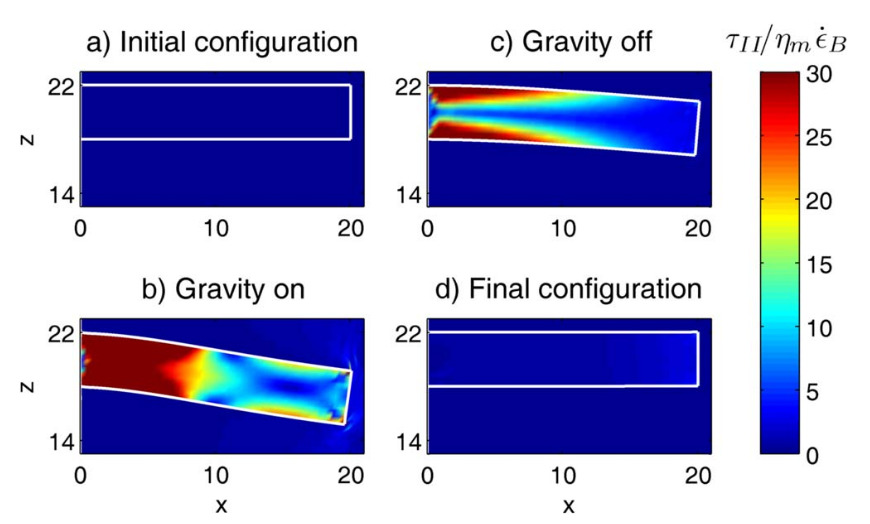
\includegraphics[width=16cm]{images/viscoelasticity/vosc15a}}\\
{\captionfont 
Reversible deformation of an elastic beam in a viscous matrix under gravity. 
(a) Unstressed initial configuration (gravity off). 
(b) Deformation of the elastic beam under gravity. 
(c) Gravity is turned off. (d) The elastic beam recovers the original rectangular 
shape with zero stress. Colors indicate the second invariant of the stress 
tensor $\tau_{II}$.}
\end{center}



%------------------------------------------------------------------------
\subsection{Elastic beam in viscous matrix (Keller, May, and Kaus, 2013)}

This benchmark comes from Appendix B of Keller et al (2013) \cite{kemk13}.

The domain is $7.5\times5$km. A dominantly elastic beam is fixed to, and protrudes horizontally 
from the left wall of the model box. 
Surrounding the elastic beam is a viscous, but inelastic fluid. 
All boundaries are free slip, except for the left wall, which is set to no slip in  
order to keep the bending beam fixed to the wall. The beam has a higher density than the surrounding fluid and 
thus will bend down elastically driven by gravity. After the beam has 
accumulated some elastic strain through bending down, gravity is switched off. 
If the stress evolution is implemented accurately, the elastic beam should now, 
free from the pull of gravity, move upwards again and restore its initial position. 

Material properties are as follows:
\begin{itemize}
\item beam: $\rho=1500$, $\eta=10^{24}$, $\mu=10^{10}$
\item fluid: $\rho=1000$, $\eta=10^{18}$, $\mu=10^{11}$
\end{itemize}

This choice of parameters leads to a Maxwell time 
$t_m = 0.32$ yr for the background fluid and Maxwell times of  
$t_m = 3.2$ Myr for the beam, meaning that the deformation in this benchmark problem, 
which occurs on a timescale of thousands to a million years, 
will lead to dominantly viscous deformation in the fluid, 
and dominantly elastic behaviour of the beam. 

Keller et al set the numerical resolution to $300\times200$ elements, 
with 16 markers per elements for stress advection. Such a resolution is  
not feasible with our simple python implementation so the resolution is
then set to $96\times64$. 

The following plot comes from \cite{kemk13}:
\begin{center}
\fbox{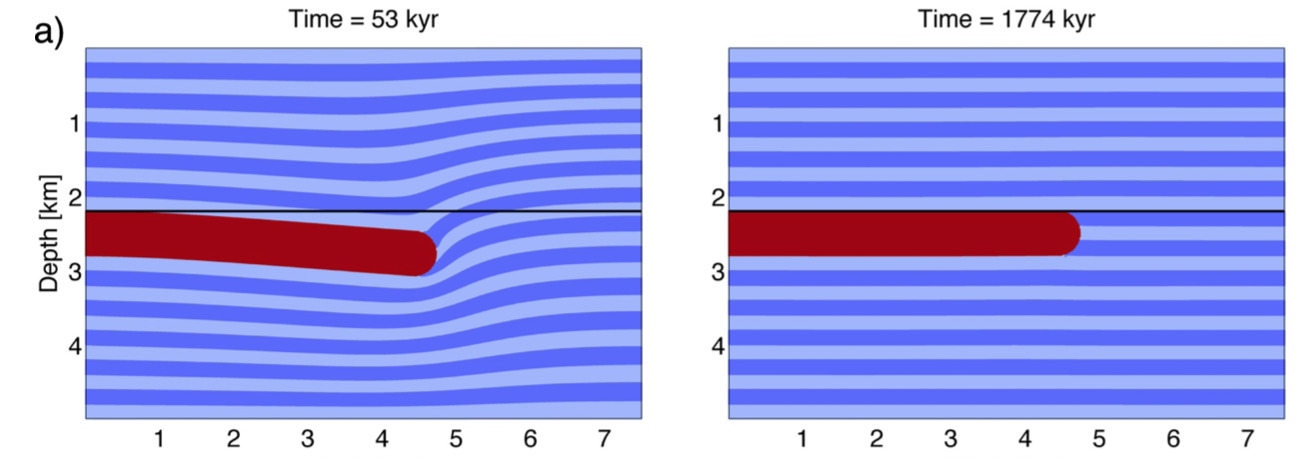
\includegraphics[width=14cm]{images/viscoelasticity/kemk13}}
\end{center}

The elastic timestep is set to $\delta t_e=100$yr and the tectonic timestep is set to the same value.
This yields $\eta_{eff}=10^{18}$ in the fluid, and $\eta_{eff}\simeq 3.15\times 10^{19}$.
After 50kyr, the gravity ($|\vec{g}|=10$) is switched off and the model is ran for another 
500kyr.


%-----------------------------------------------
\subsection{Cantilever Beam (Moresi et al, 2002)}

The following text is 100\% taken from \textcite{modm02}. 

``A simple example is the gravitational loading of a thick, heavy beam of
viscoelastic material. The beam dimensions were 0.1 wide by 0.75 thick, with
viscosity of $10^7$, elastic shear modulus of $10^6$, density 2500 and perfectly rigid
support at one end. Loading was conducted in a very low viscosity ($\eta=0.01$)
compressible, background medium. The beam was loaded by applying a
gravitational body force at time $t=0$, which was subsequently switched off when
the deflection of the beam reached 0.35 at the unsupported end. We varied the
intensity of the gravitational acceleration from $g=5$ to $g=500$ to produce
responses with different characteristic times(owing to the viscous resistance of the
embedding medium).''

``Figure 3 shows superimposed snapshots of the loading (a) and unloading (b) of
the beam for $g=500$. Under such strong loading, the beam reached the maximum
allowed deflection very rapidly (relative to the viscous relaxation time) and the load
was then released. Once unloaded, unrelaxed elastic stress in the beam caused it to
straighten out. The loading time was sufficiently short that negligible viscous
deformation occurred, allowing the beam to return to within 0.001 of its original
location.''

\begin{center}
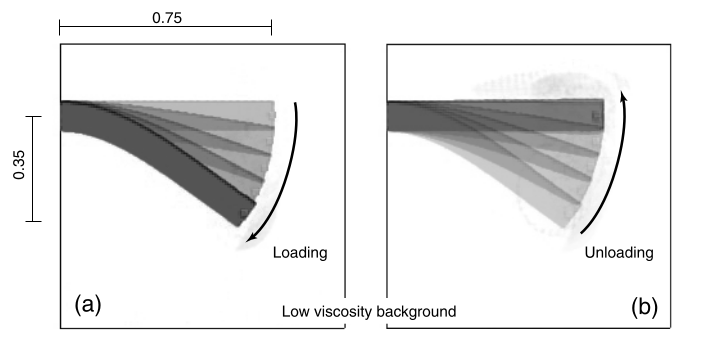
\includegraphics[width=10cm]{images/viscoelasticity/modm02f}\\
{\captionfont A heavy viscoelastic beam of length 0.75 is subjected to a gravitational 
load at time $t=0$ which is released when the end deflection reaches 0.35. The superimposed 
configurations correspond to approximately equal time intervals.}
\end{center}


``The deflection of the mid-point at the unsupported end of the beam is shown in
Figure 4 for the range of loading intensities. Under light loading ($g=5,9$) the
initial deflection of the beam is rapid, dominated by elastic deformation of the beam
and the viscous resistance of the embedding medium. In the absence of viscous
terms, the elastic stresses in the beam would come to an equilibrium with
gravitational loading. However, After $t=0.0005$, there was a small but observable
rate of end deflection still occurring through gradual viscous relaxation of the
elastic stresses. When the gravitational load was released, this relatively long period
of viscous relaxation resulted in a permanent deflection of 0.1.In the case $g=5$, we
observed the initial rapid deflection due to elastic deformation of the beam, and the
gradual deflection after $t=0.0005$. However, the rate of viscous deformation was so
low that the end deflection of 0.35 was not reached within the time limit imposed
for the experiment.''


\begin{center}
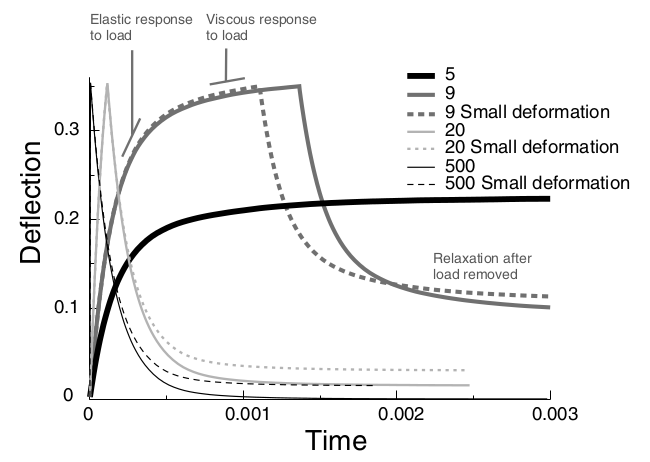
\includegraphics[width=10cm]{images/viscoelasticity/modm02g}\\
{\captionfont Deflection as a function of time for the heavy viscoelastic beam for 
numerous different load intensities. Dashed lines correspond to simulations where 
the corotational terms were omitted from the computation of the stress rate.}
\end{center}


``The fast-loading cases, $g=20,500$ suffered very little viscous relaxation
before unloading occurred. The stress state at the time of unloading was therefore
similar for the two cases. Although the loading rates were very different, the
unloading displacement curves remained almost parallel until most the elastic stresses
had been released.''

``To demonstrate the importance of computing the stress update correctly, we ran
the simulations omitting the corotational terms in the stress rate (dashed lines in
Fig. 4). The results were qualitatively similar, however the cumulative result of not
allowing for stress rotation was greater viscous deformation. This resulted in larger
permanent deformation at the end of the simulation, particularly noticeable in the
$g=500$ case where there is virtually no final deformation if the corotational stress
rate is computed correctly.''





%---------------------------------------------------------------------------------
\subsection{Boxcar load on an incompressible viscoelastic lithosphere (Wu, 1992)}

{\color{orange} fully incompressible}

This originates in \textcite{wu92} (1992).
The domain is $2500~\si{\km}$ long and it is either 
a halfspace in the vertical direction 
or a channel of $100~\si{\km}$ width. 
The material is characterised by 
$\rho=3400~\si{\kg\per\cubic\meter}$, 
Young's modulus $E=\SI{1.13e11}{\pascal}$ 
and a Poisson ratio $\nu=0.5$ with $|\vec{g}|=9.82~\si{\meter\per\square\second}$.
The author explores the effect of a linear viscous mantle vs dislocation creep.
Time evolution/relaxation figures are available.

\begin{center}
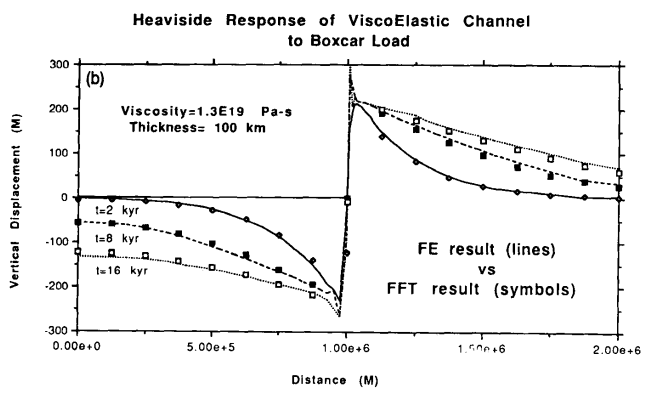
\includegraphics[width=12cm]{images/viscoelasticity/wu92}\\
{\captionfont The Heaviside responses of linear viscoelastic earth models calculated 
with the finite element method (lines) are compared to those computed using the conventional 
transform method (symbols). For a $100~\si{\km}$ thick channel.}
\end{center}

also explore Wu \& Peltier \cite{wupe82} (1982).


%------------------------------------------------------------------------------------------
\subsection{Boxcar load on an incompressible viscoelastic lithosphere (Hampel et al, 2019)}

\textcite{halk19} (2019)

{\color{orange} fully incompressible}

\begin{center}
\fbox{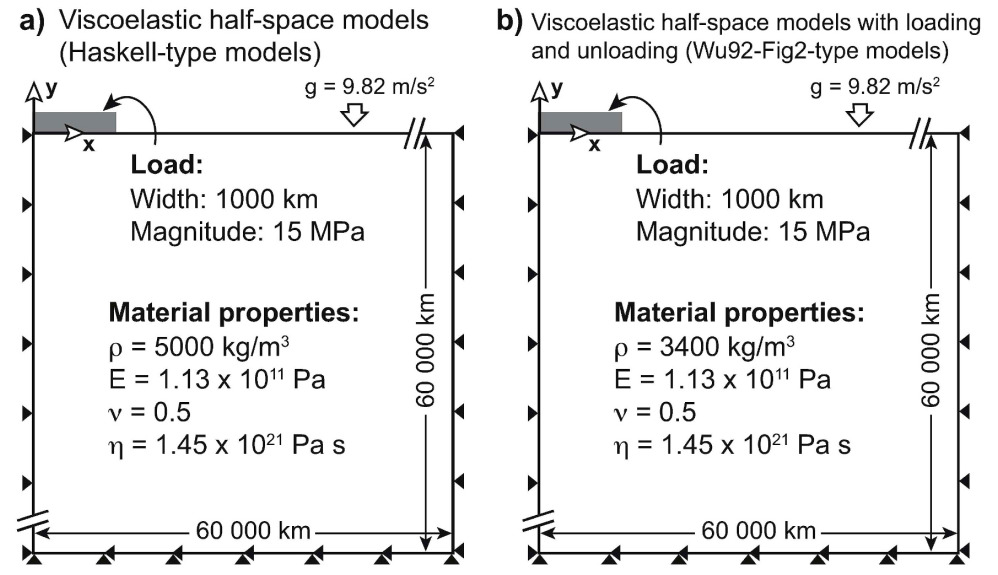
\includegraphics[width=12cm]{images/viscoelasticity/halk19}}\\
{\captionfont 
a) Viscoelastic Haskell-type half-space models. b) Viscoelastic  half-space models used for modelling loading and subsequent
unloading (after Wu, 1992; his Fig. 2). Both model types are meshed with 25x25 km large linear, rectangular plane strain elements suitable for incompressible materials. 
The same mesh and element type are used in all model runs. All viscoelastic half-space models have the same boundary conditions (indicated by black triangles): the model bottom is fixed in both the vertical and horizontal direction while the model sides are fixed in the horizontal direction. In models with an elastic foundation (Table 1), it is applied to the model surface. Abbreviations for model parameters are $\rho$ density, $E$ Young's modulus, $\nu$ Poisson's ratio, $\eta$ viscosity and $g$ acceleration due to gravity. Following Wu (1992), we use a value of $g = 9.82 m/s^2$ in the viscoelastic
half-space models. 
In all models, the load is applied (and removed, if applicable) instantaneously. The magnitude of the applied load is 15 MPa, which is equivalent to about 1.5 km of ice. The left end of
the load coincides with the origin of the coordinate system at the beginning of the model run. See text for details.
}
\end{center}


%-----------------------------------------------------------------------------------------
\subsection{Two-layer lithosphere under lateral stress (Kusznir and Bott, 1977)}

The domain is a $\SI{2000}{\km}\times\SI{80}{\km}$ Cartesian box. 
However since there is a vertical axis of symmetry it is then reduced to 
$\SI{1000}{\km}\times\SI{80}{\km}$.
It consists of two layers: the top layer is $\SI{20}{\km}$ thick and is 
purely elastic characterised by a Young's modulus $E=\SI{1.7e11}{\newton\per\square\meter}$ and a Poisson ratio $\nu=0.25$.
The lithosphere below is then $\SI{60}{\km}$ thick and is characterised by an elasto-viscous rheology. The elastic parameters are identical to the upper layer while the viscosity is set to $\eta_0=\SI{1e23}{\pascal\second}$.

We arbitrarily design the right side as being the axis of symmetry and the 
boundary condition on that side are then free slip. On the left side a uniform 
horizontal stress $T$ is applied at time t=0.
The viscous drag of the asthenosphere below is neglected and the authors do not 
mention the bottom of the domain deforming so 
we'll also impose free slip boundary conditions at the bottom.

Fig.~4 of the paper shows the vertical displacement of the upper layer so we will use 
a free surface boundary condition at the top. 
The model is ran for $\SI{1}{\mega\year}$.

\begin{center}
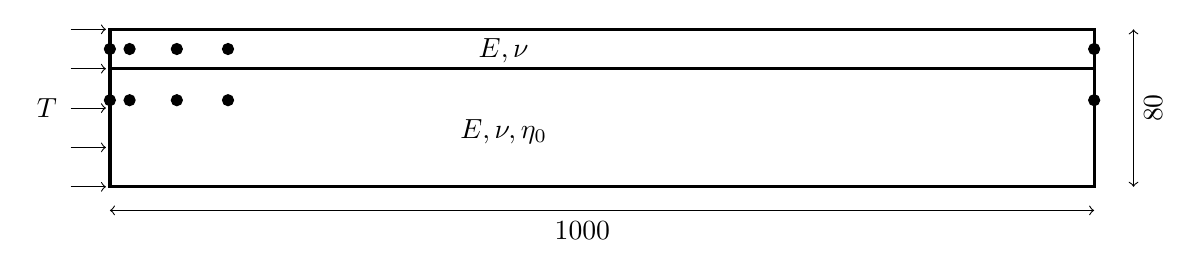
\begin{tikzpicture}
%\draw[step=0.5cm,gray,very thin] (0,0) grid (15,4); %background grid
\draw[very thick] (1,1)--(13.5,1)--(13.5,3)--(1,3)--cycle;  
\draw[very thick] (1,2.5)--(13.5,2.5);  
\draw[<->] (1,0.7)--(13.5,0.7);
\draw[<->] (14,1)--(14,3);
\node[] at (7,0.45) {$\SI{1000}{\km}$};
\node[rotate=90] at (14.25,2) {$\SI{80}{\km}$};
\node[] at (6,2.73) {$E,\nu$};
\node[] at (6,1.7) {$E,\nu,\eta_0$};
\draw[->] (0.5,3)--(0.95,3);
\draw[->] (0.5,2.5)--(0.95,2.5);
\draw[->] (0.5,2)--(0.95,2);
\draw[->] (0.5,1.5)--(0.95,1.5);
\draw[->] (0.5,1)--(0.95,1);
\node[] at (0.2,2) {$T$};

\filldraw[black] (1,2.75) circle (2pt);
\filldraw[black] (1,2.1) circle (2pt);

\filldraw[black] (1.25,2.75) circle (2pt);
\filldraw[black] (1.25,2.1) circle (2pt);

\filldraw[black] (1.85,2.75) circle (2pt);
\filldraw[black] (1.85,2.1) circle (2pt);

\filldraw[black] (2.5,2.75) circle (2pt);
\filldraw[black] (2.5,2.1) circle (2pt);

\filldraw[black] (13.5,2.75) circle (2pt);
\filldraw[black] (13.5,2.1) circle (2pt);
\end{tikzpicture}
\end{center}


After a thorough read of the paper, I have noticed quite a few problems:
\begin{itemize}
\item the paper is old and has been digitized but the figures are missing a lot of lines/shades/points ... this could be remedied by finding the article in a library.
\item in the intro it is stated: "Here we investigate the response of a lithosphere divided into upper elastic and lower uniform visco-elastic layers to simple boundary force and body force systems." The authors later talk about 'isostatic forces' opposing flexure. This means that buoyancy forces should be taken into account but there is no information about densities or gravity values!
\item little uncertainty about boundary conditions. is it free slip or no-slip on the right side ? Looking at fig 4, it looks like the vertical displacement is zero at x=1000km?
\item a Maxwell elasto-viscous rheology is used but this is only mentioned in the Appendix
\item the dimensions of the thinned or thickened areas is simply not mentioned. 
\item Fig~1 shows triangular elements. No mention is made of resolution, type of element, ndofs, resolution tests, any numerical detail whatsoever. Given the age of the paper, I would guess $P_1$
elements.
\item In the appendix they equate the viscous strain rate to $\sigma/4\eta$. Why 4 ?
\item it is also not clear whether the domain is ALE or fully Lagrangian: does it shorten?
\item the value of $T$ is never specified!
\item the paper was published 45 years ago, it is extremely unlikely any of the two authors is still available 
\end{itemize}

\begin{center}
\fbox{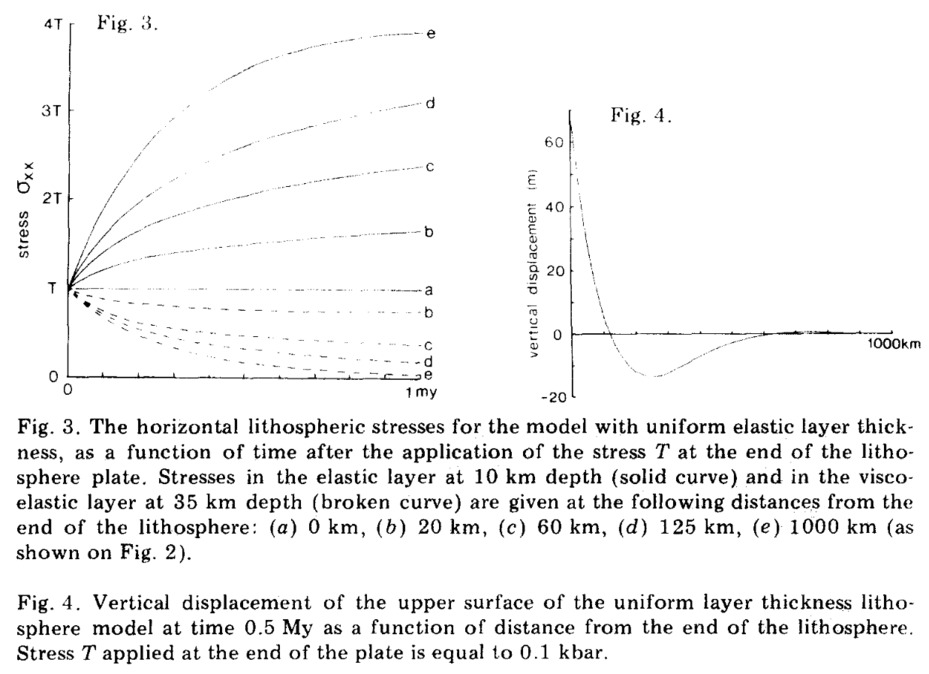
\includegraphics[width=16cm]{images/viscoelasticity/kubo77}}\\
{\captionfont Taken from \textcite{kubo77}. Measurement locations are indicated on 
the setup figure above. probably should be reversed}
\end{center}



%---------------------------------------------------------------------------
\subsection{Parallel-Plate Viscometer Problem (SNAC manual) \label{v-e-snac}}

A parallel-plate viscometer problem is simulated, in which viscoelastic material is squeezed between two
parallel plates. The plates are moving at a constant velocity, $v_0$. Each plate has the length of $2L$ and 
is at a distance $2h$ from the other. No slip is assumed between the material and the plates. The approximate
analytical solution is given in the book by \textcite{jaeg69} (1969).

Model Setup: $L = 10~\si{\meter}$, $h=5~\si{\meter}$, viscosity $\eta=10^9~\si{\pascal\second}$, 
bulk modulus $K= 1.5~\si{\giga\pascal}$, shear modulus $\mu = 500~\si{\mega\pascal}$,
$v_0 = 10^{-4}~\si{\meter\per\second}$, $dt = 1~\si{\second}$ (results compared after 500 time steps),
mesh size: $20\times 10~\si{\meter}$, each element is a $1~\si{\meter}$ cube.

Due to the assumption of the original problem setup, artificial forces should be added to left and right
surfaces.

\begin{center}
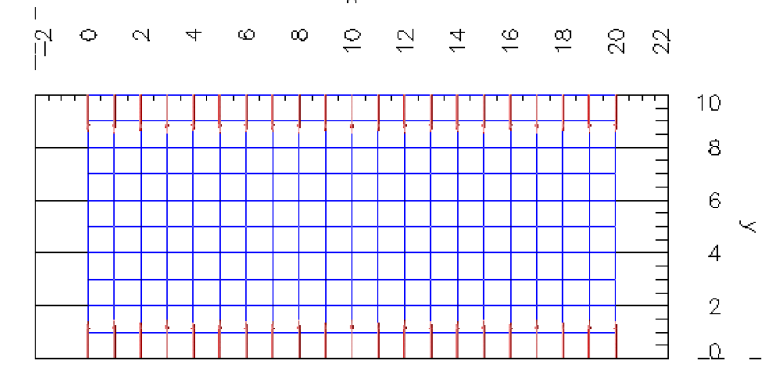
\includegraphics[width=8cm]{images/viscoelasticity/snac_5}
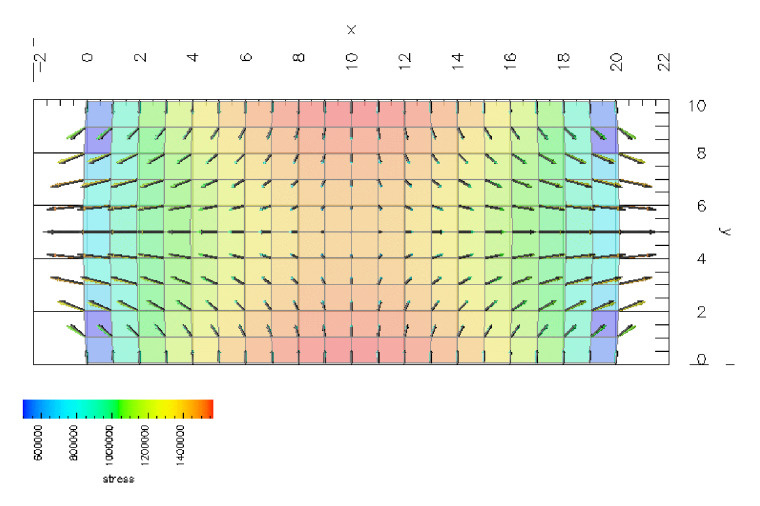
\includegraphics[width=8cm]{images/viscoelasticity/snac_6}\\
{\captionfont 
Left: The initial mesh (blue) with the velocity boundary condition (red arrows);
Right: The second invariant of stress and velocities plotted on the deformed mesh. Colored arrows are
for SNAC’s solution, black ones for the analytic solution.}
\end{center}

$K=\lambda + \frac23 \mu$ so $\lambda=\frac{3500}{3}MPa$ ?

From wikipedia\footnote{\url{https://en.wikipedia.org/wiki/Lame_parameters}}
\[
\nu = \frac{3K-2\mu}{2(3K+\mu)} 
= \frac{4500-2*500}{2(4500+500)}
= \frac{3500}{10000}
= 0.35
\]
so we find that the material is {\color{orange} compressible $\nu=0.35$}

\[
E=\frac{9K\mu}{3K+\mu} 
=\frac{9*1500*500 MPa^2}{4500+500 MPa}
=\frac{9*1500*500}{5000} MPa
= 1350Mpa
\]


%..........................................................
\subsection{Relaxation after extention (Hassani syllabus)}

{\color{orange} compressible $\nu=0.25$}

Un essai de relaxation consiste à imposer à un instant donné une déformation que 
l’on maintient constante par la suite. On observe alors comment évolue la contrainte au cours du temps.

The setup of the experiment is shown in the following figure:

\begin{center}
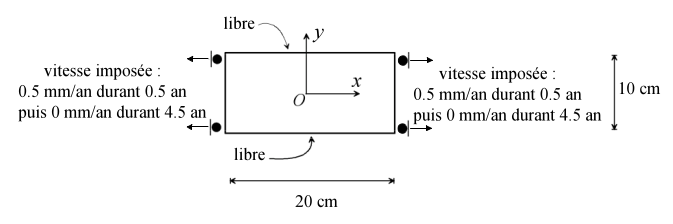
\includegraphics[width=9cm]{images/viscoelasticity/hassani_1}
\end{center}

The total duration of the experiment is $T=\SI{5}{\year}\simeq \SI{15.75e7}{\second}$.
The duration of the loading is $T/10=\SI{6}{months}$ while the duration 
of the subsequent relaxation is then $9T/10\simeq 4.5~\si{\year}$.

The loading velocity is $v=\SI{1}{\mm\per\year}\simeq \SI{3.17e-11}{\meter\per\second}$.
The sample has size $L\times L/2 = 20\times10\si{cm}$ and 
the strain rate is then $v/L \simeq \SI{1.5e-10}{\per\second}$.
Young's modulus is set to \SI{1e11}{\pascal} and the Poisson ratio is 0.25, i.e.
$\mu=40~\si{GPa}$. The viscosity is set to $\eta_0=\SI{1e18}{\pascal\second}$.
The Maxwell time is then $t_M=\eta/\mu=0.8~\si{\year}$, which is also the time it takes 
to reduce the maximum stress by a factor $e$.

\begin{center}
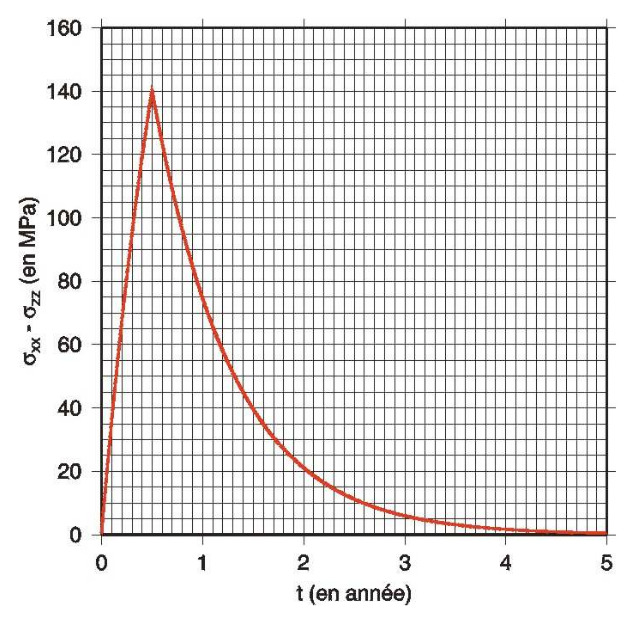
\includegraphics[width=6cm]{images/viscoelasticity/hassani_2}
\end{center}







%-------------------------------------------------------------------------
\subsection{Role of elasticity in slab bending (Fourel et al, 2014)}

\fullcite{fogm14}

\begin{center}
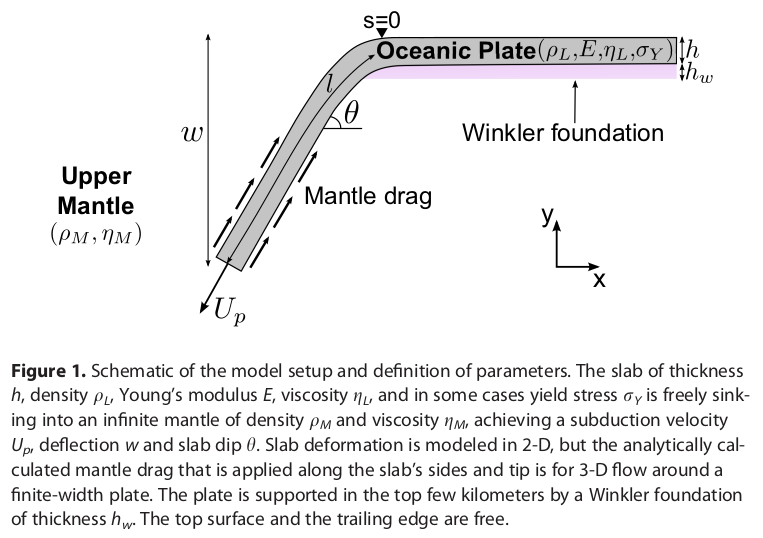
\includegraphics[width=8cm]{images/viscoelasticity/fogm14b}
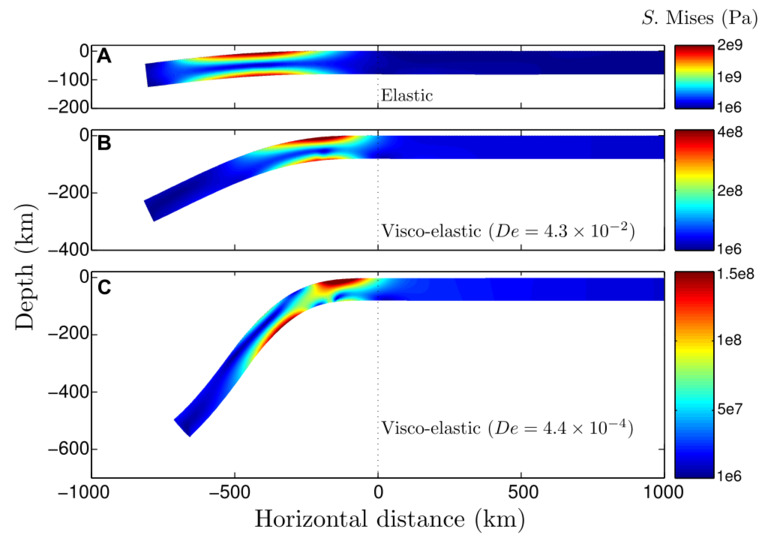
\includegraphics[width=8.5cm]{images/viscoelasticity/fogm14c}\\
\end{center}



%-------------------------------------------------------------------------
\subsection{Shear test in 2D (Farrington et al, 2014)}

\fullcite{famc14}

This experiment consists of a viscoelastic material undergoing simple shear at a constant 
rate from a time $t_0$ though to $t_{max}$. At $t_{max}$, the shearing velocity is taken 
to zero using a no-slip velocity boundary condition. The viscoelastic stresses then decay
with time while the material deformation rate remains zero. The $xy$ component of stored 
stress, i.e. the nonviscous portion of the total stress, is given by
\begin{align}
\tau_{xy}^{stor} 
&= 
\exp -\frac{\mu}{\eta}t 
\left(
C_2 \cos\left( \frac{Vt}{h}\right)
-C_1 \sin\left( \frac{Vt}{h}\right)
\right)
-C_2 & \textrm{if} \; t<t_{max} \nn\\
&= \left[\exp -\frac{\mu}{\eta}t_{max} 
\left(
C_2 \cos\left( \frac{Vt}{h}\right)
-C_1 \sin\left( \frac{Vt}{h}\right)
\right)
-C_2 \right] \exp -\frac{\mu}{\eta}(t-t_{max})
& \textrm{if} \; t>t_{max} 
\end{align}
where $V$ is the shear velocity along the top wall boundary, 
$h$ is the height of the box,
\[
C_1=-\frac{V^2 \eta^2 \mu}{\mu^2 h^2 + V^2 \eta^2}
\]
\[
C_2=-\frac{Vh\eta \mu^2}{\mu^2 h^2 + V^2 \eta^2}
\]

\begin{center}
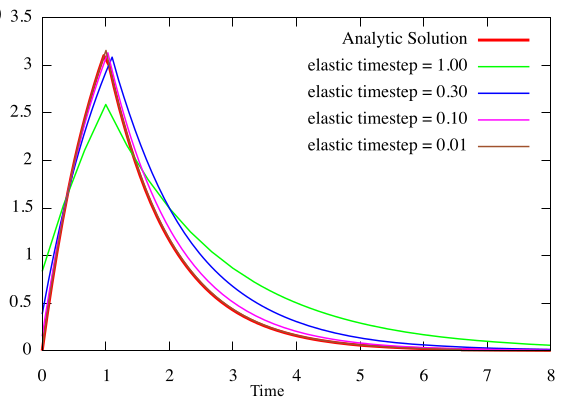
\includegraphics[width=8cm]{images/viscoelasticity/famc14a}\\
\captionfont{The xy component of dimensionless stored stress with dimensionless time 
for the 2-D viscoelastic material undergoing simple shear and relaxation. Nondimensional 
material parameters of $\eta=10^2$, $\mu=10^2$, $t_M=1$, $V=0.05$, $h=1$ 
with $\Delta t_e\in[0.01,1]$ and $\Delta t_c=\frac13 \Delta t_e$.
}
\end{center}

Figure above shows the resulting xy component of the deviatoric stored stress term for a 2-D viscoelastic material across a range of $\Delta t_e$. 
At longer $\Delta t_e$, the stored stress appears under resolved, indicating these larger elastic time step values capture dynamics that occur on time scales approximately equal to or greater than the Maxwell relaxation time, that is with a portion of viscous deformation. For shorter $\Delta t_e$,
the numerically calculated stress approaches the analytic solution, indicating that the elastic time step is
sufficiently small to fully capture the elastic stored stresses produced within the material under the
applied strain rate.


%-------------------------------------------------------------------------
\subsection{Tortion test in 3D (Farrington et al, 2014)}

\fullcite{famc14}

insert here eq 9 of paper

The analytic solution outlined by equation (9) can be extended from this 
essentially 1-D test into 3-D by applying the shear velocity in the x-z plane. 
Testing of the full viscoelastic implementation including the
rotation terms is possible by placing this 3-D shear test in a 
coordinate system under going solid body rotation. 

\begin{center}
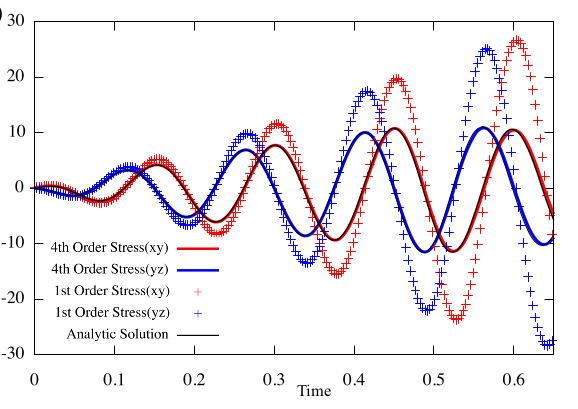
\includegraphics[width=8cm]{images/viscoelasticity/famc14b}\\
\captionfont{
The $xy$ and $yz$ stress components of a material undergoing simple shear within 
a 3D rotating reference frame. Nondimensional material parameters of 
$\eta=100$, $\mu=100$, $\alpha=1$, $V=0.3$, $h=1$, $t_{max}=0.5$
and $\omega=42$. Note the coordinate system for this test has the $y$ axis in the vertical 
with the $z$ axis in plane. Results for a first (crosses) and 
fourth- (lines) order accurate Jaumann stress rate integration scheme are shown 
in comparison to the analytical solution (black) given by equation (9) within the rotating frame.
}
\end{center}

Figure above shows the evolution of the stress in comparison to the analytical solution of equation (9)
placed within the rotating frame. The rotating frame is achieved by imposing a velocity boundary condition
of a constant solid body rotation about the y axis in addition to the shearing rate. The stress within this
rotating frame is given by equation (9), with the stress in the nonrotating frame found by 
applying a rotation matrix, $R$, to the nonrotating stress solution. 
That is, $\tau=R^{-1}\tau'R$, where $'$ denotes the rotated frame, $R$ is
the rotation matrix about the y axis given by 
\[
R= \left(
\begin{array}{ccc}
\cos\theta &0 & \sin\theta \\
0 & 1 & 0 \\
-\sin\theta & 0 & \cos\theta
\end{array}
\right)
\]
with $\theta=\omega t$, $\omega$ being the dimensionless rotation rate. 
The stress components shown in Figure 1b from within the 
nonrotating frame can then be given by $\tau^{stor}_{xy}=\tau^{stor'}_{xy} \cos\theta$
and $\tau^{stor}_{yz}=\tau^{stor'}_{yz} \sin\theta$.
It can be seen that, using a higher-order Jaumann stress rate advection scheme 
results in accurate stress advection and rotation within the full
3-D space plus time domain. It should be noted here that the velocity field used in 
this test was chosen to rigorously test the rotational terms in equation (6). 
Whether these rotational terms are required for individual models is dependent upon 
the model setup. For subducting slabs at a constant curvature, the individual 
parcels of material experience purely rotational effects, accounting for this within the stress history term
would then be required for consistency.

{\color{red} finish!}










%------------------------------------------------
\subsection{Cylindrical tunnel (Segall book ?)}

{\color{orange} compressible $\nu=0.25$}

communicated to me by L .van de Wiel.

This is a cylindrical tunnel (2D magma chamber) in an infinite space, with certain radius.
The material close around the hole is warm, and and such viscous. The material further from the hole is cold, and purely elastic. (accomplished by setting and absurdly high viscosity) 
There is a clear transition radius between the two properties
The hole contains a pressure, causing the space to expand.

After the initial elastic deformation, viscous deformation continues in the viscous region of the domain.
I have the implementation of the analytical solution attached to save you time.

See plot with radial deformation for t=0 (green), t=300s (red), t=600s (blue), and t=3000s (black).
thin line is analytic, points are numeric.
(with parameters and size parameters as in analytic.f)

\begin{center}
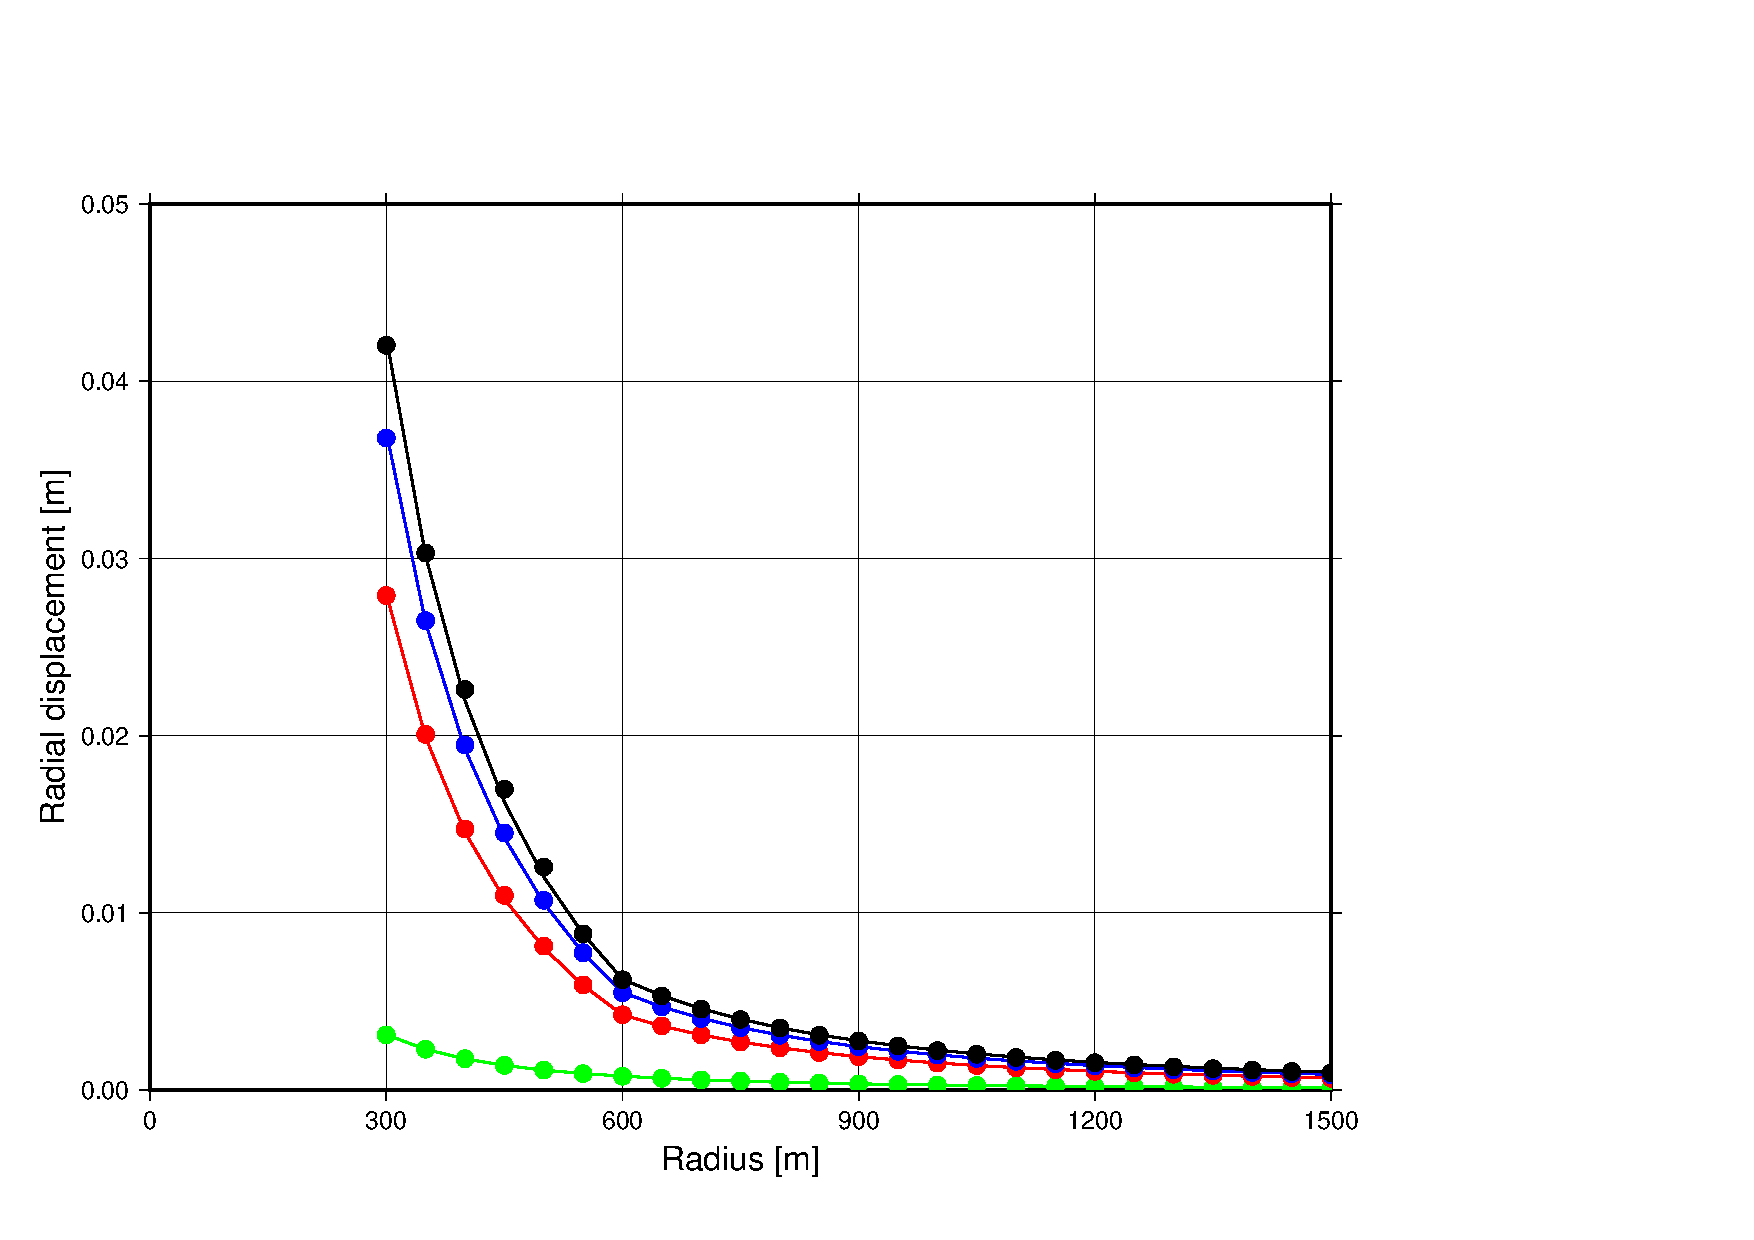
\includegraphics[width=8cm]{images/viscoelasticity/radialDisp}
\end{center}


%--------------------------------------------------------------------
\subsection{Gravitational instability of an elastically compressible
viscoelastic Maxwell solid overlying an inviscid incompressible fluid (Burov \& Molnar, 2008)}

\fullcite{bumo08}

\begin{center}
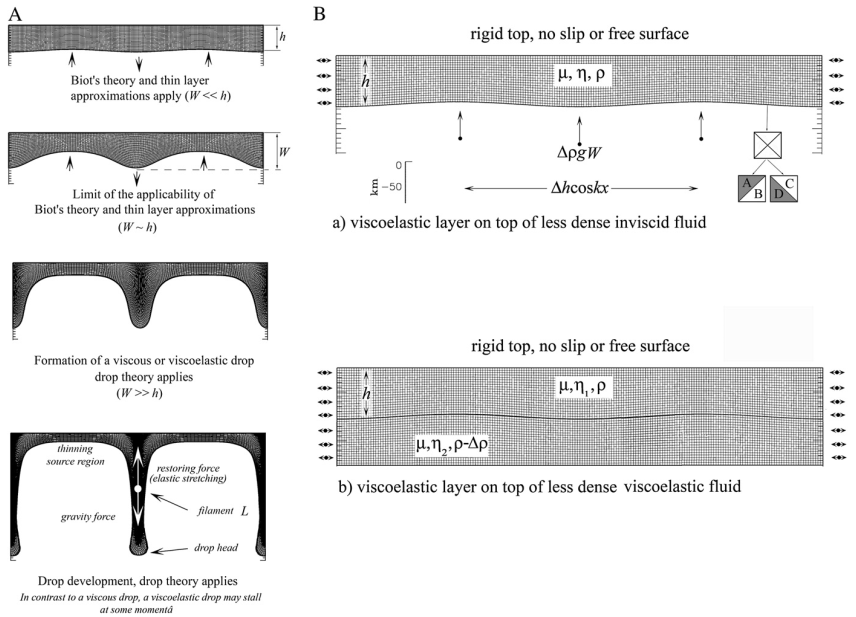
\includegraphics[width=12cm]{images/viscoelasticity/bumo08}\\
{\captionfont A) Sequence of different stages of development of a Rayleigh–Taylor instability in a viscoelastic layer of thickness h overlying an inviscid fluid of lower density. B) Numerical setup for experiments. }
\end{center}

%--------------------------------------------------------------------------------
\subsection{craton stability using a viscoelastic rheology (Beuchert et al, 2010)}

\fullcite{beps10}

\begin{center}
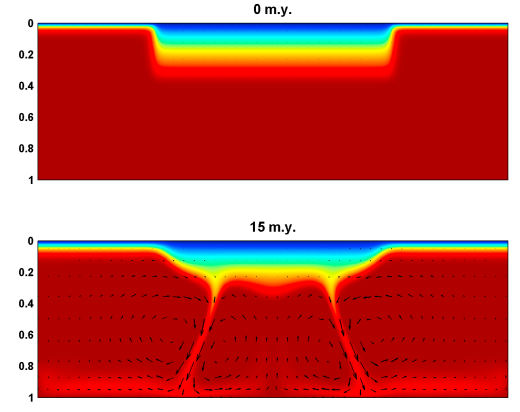
\includegraphics[width=7cm]{images/viscoelasticity/beps10d}
\end{center}






\newpage
%..........................................................
\subsection{Relevant literature \& various notes}



\begin{itemize}
\item \underline{convection of viscoelastic fluids}: 
\textcite{hard91}, \textcite{zhgm96},
\textcite{mure05}, \textcite{likh05a}, \textcite{likh05b}, \textcite{fukk08}.

\item stress buildup associated with viscoelastic rheology: 
\textcite{kubo77}, \textcite{kupa84}, \textcite{pocp93}, \textcite{mapo09}.

\item viscoelastic effects on geodynamical pbs involving gravitational instability 
\textcite{pocp93,kabe07,bumo08,scbe08}, \textcite{hamy95}.

\end{itemize}

\textcite{famc14} states 
``Funiciello et al. [2003] implemented a viscoelastic rheology in numerical models of subduction, performing a
range of numerical simulations to investigate its effect on subducting slab dynamics. Similar methodologies have addressed the details of viscoelastic stress within the bending zone during subduction, although a comparison between viscous and viscoelastic rheology was lacking [Capitanio et al., 2009; Capitanio and Morra, 2012].
Muhlhaus and Regenauer-Lieb [2005] and Moresi et al. [2002] have studied the role of elasticity in mantle convection, comparing the viscous case to that of viscoelastic, and Kaus and Becker [2007] discussed the effect of elasticity on layered Rayleigh-Taylor instabilities. However, a systematic study into the effects of elastic stresses on models of free subduction has yet to be completed. Morra and Regenauer-Lieb [2006], Funiciello et al. [2003], Capitanio et al. [2007], Yamato et al. [2007], and Royden and Husson [2006] have included a viscoelastic slab in subduction models, without explicitly studying the effects of the elastic component across a range of parameters.''



\newpage
\subsection{appendix: Equations in hard91\label{ve_hard91}} 
\fullcite{hard91}

%-------------------
\begin{multicols}{2}
\begin{center}
{\bf Article excerpts}
\\ 
{\bf Notes and remarks}
\end{center}
\end{multicols}


\begin{multicols}{2}
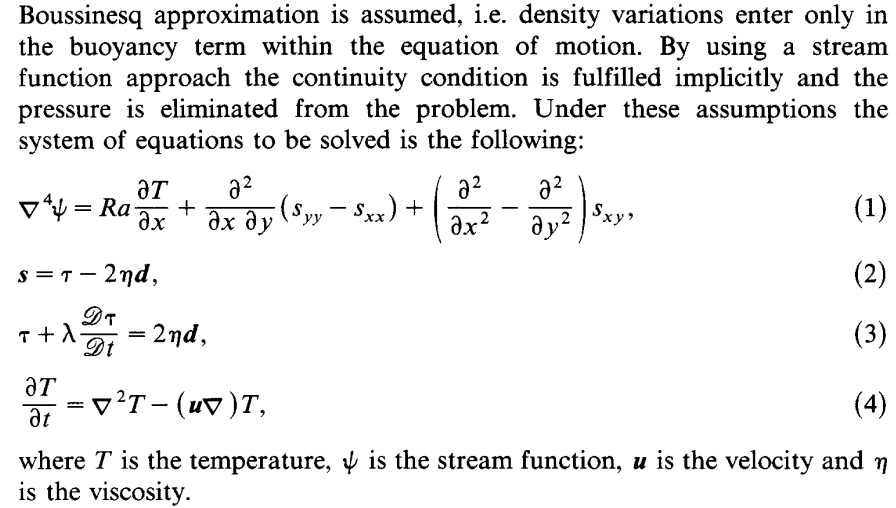
\includegraphics[width=8.3cm]{images/viscoelasticity/hard91_a}\\
What is ${\bm s}$ here? it is defined as "non-Newtonian 
contribution to the stress tensor ${\bm\tau}$.
\[
\frac{{\bm \tau}}{2\eta} + \frac{\lambda}{2\eta}\frac{{\cal D}{\bm \tau}}{{\cal D}t}
=\dot{\bm\varepsilon}
\]
Probably here $\lambda=\eta/\mu$ (see \ref{ve_momy93}), so that 
\[
\frac{{\bm \tau}}{2\eta} + \frac{1}{2\mu}\frac{{\cal D}{\bm \tau}}{{\cal D}t}
=\dot{\bm\varepsilon}
\]
\end{multicols}

\begin{multicols}{2}
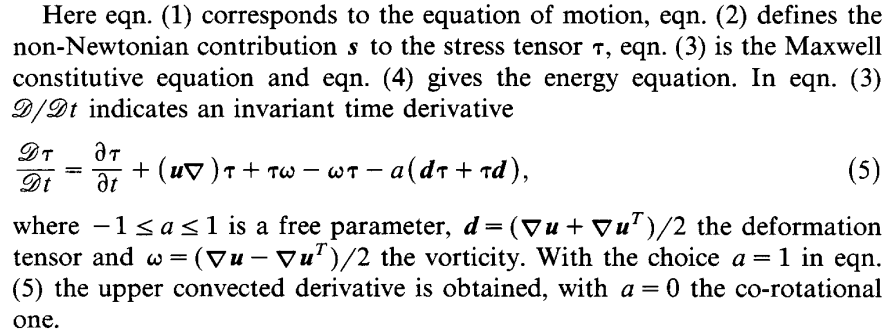
\includegraphics[width=8.3cm]{images/viscoelasticity/hard91_b}\\
\[
\frac{{\cal D}{\bm \tau}}{{\cal D}t}
=
\frac{\partial {\bm \tau}}{\partial t}
+(\vec\upnu\cdot \vec\nabla) {\bm \tau}
+ {\bm \tau}\cdot \dot{\bm\omega} - \dot{\bm \omega}\cdot {\bm \tau}
- a (\dot{\bm\varepsilon} \cdot {\bm \tau} + {\bm \tau}\cdot \dot{\bm\varepsilon})
\]
\end{multicols}

\begin{multicols}{2}
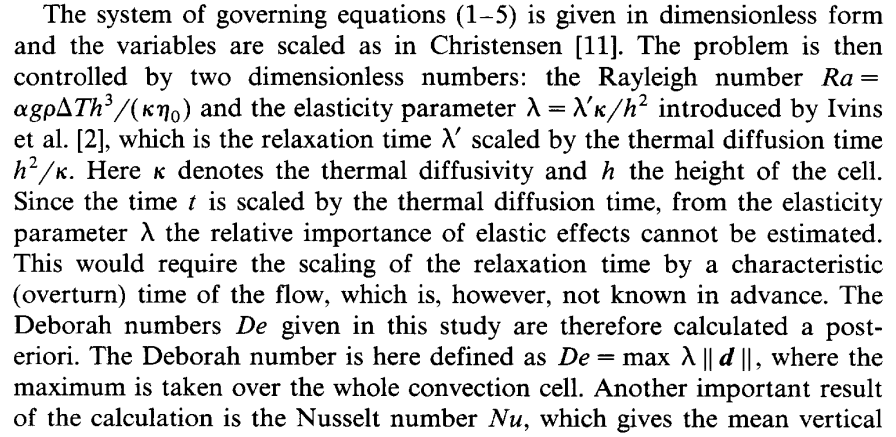
\includegraphics[width=8.3cm]{images/viscoelasticity/hard91_c}\\
\end{multicols}


\newpage
\subsection{appendix: Equations in momy93\label{ve_momy93}} 
\fullcite{momy93} \\

Note that Harder is co-author here and author of the previous subsection \label{ve_hard91}
which explains the overlap in notations.

%-------------------
\begin{multicols}{2}
\begin{center}
{\bf Article excerpts}
\\ 
{\bf Notes and remarks}
\end{center}
\end{multicols}

%-------------------
\begin{multicols}{2}
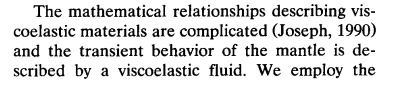
\includegraphics[width=7cm]{images/viscoelasticity/momy93a}\\
\end{multicols}

%-------------------
\begin{multicols}{2}
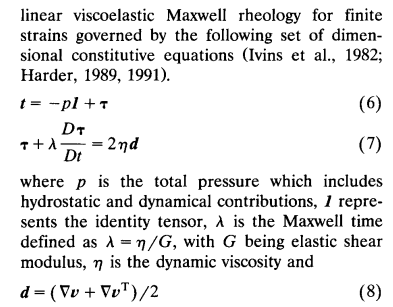
\includegraphics[width=7cm]{images/viscoelasticity/momy93b}\\
\[
{\bm \sigma} = -p {\bm 1} + {\bm \tau}
\]
\[
{\bm \tau}  + \frac{\eta}{\mu} \frac{{\cal D} {\bm \tau}}{{\cal D}t} = 2\eta \dot{\bm \varepsilon}
\Rightarrow
\frac{1}{2\eta} {\bm \tau}  + \frac{1}{2\mu} \frac{{\cal D} {\bm \tau}}{{\cal D}t} 
=  \dot{\bm \varepsilon}
\]
\end{multicols}

%-------------------
\begin{multicols}{2}
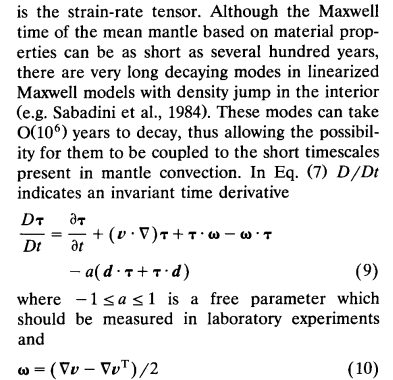
\includegraphics[width=7cm]{images/viscoelasticity/momy93c}\\
\[
\frac{{\cal D} {\bm \tau}}{{\cal D}t} = \frac{\partial {\bm \tau}}{\partial t}  
+ (\vec\upnu \cdot \vec\nabla) {\bm \tau} 
+ {\bm \tau} \cdot \dot{\bm \omega} + \dot{\bm \omega} \cdot {\bm \tau}
- a (\dot{\bm \varepsilon} \cdot {\bm \tau} + {\bm \tau} \cdot \dot{\bm \varepsilon})
\]
\[
\dot{\bm \omega} = \frac12 (\vec\nabla \vec\upnu  - \vec\nabla \vec\upnu^T  ) 
\]
\end{multicols}



\newpage
\subsection{appendix: Equations in modm01\label{ve_modm01}} 

\fullcite{modm01}

%-------------------
\begin{multicols}{2}
\begin{center}
{\bf Article excerpts}
\\ 
{\bf Notes and remarks}
\end{center}
\end{multicols}


\begin{multicols}{2}
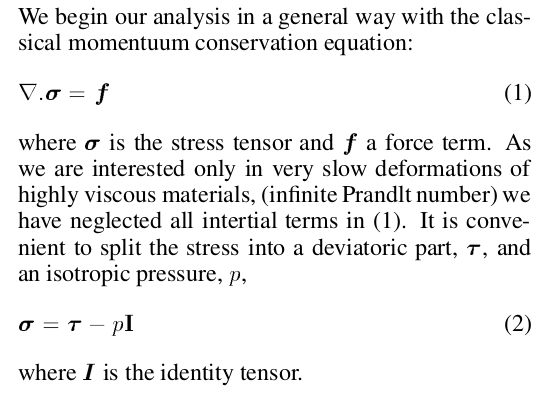
\includegraphics[width=8.25cm]{images/viscoelasticity/modm01a}\\
\[
\vec\nabla \cdot {\bm \sigma} + \vec{f} = \vec{0}
\]
\[
{\bm \sigma} = -p {\bm 1} + {\bm \tau}
\]
\end{multicols}

\begin{multicols}{2}
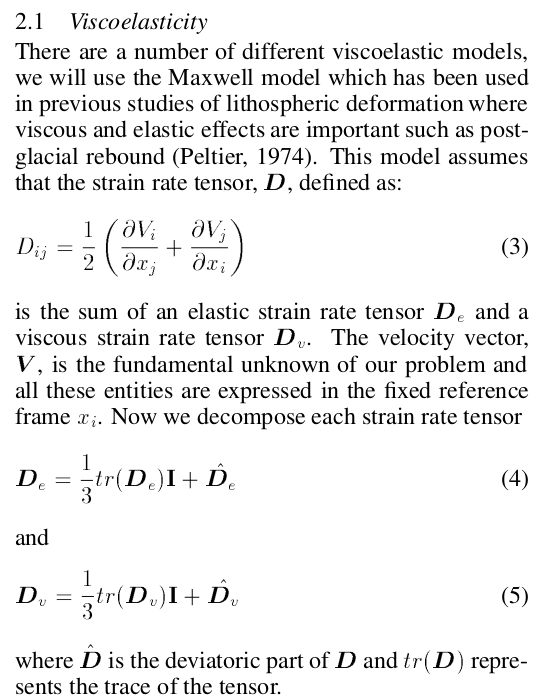
\includegraphics[width=8.25cm]{images/viscoelasticity/modm01b} \\
\[
\dot{\bm \varepsilon} = \frac12 (\vec\nabla \vec\upnu  + \vec\nabla \vec\upnu^T  ) 
\]

\[
\dot{\bm \varepsilon}_e = \frac13 {\rm tr}(\dot{\bm \varepsilon}_e) {\bm 1} + \dot{\bm \varepsilon}_e^d 
\]
\[
\dot{\bm \varepsilon}_v = \frac13 {\rm tr}(\dot{\bm \varepsilon}_v) {\bm 1} + \dot{\bm \varepsilon}_v^d 
\]
\end{multicols}

\begin{multicols}{2}
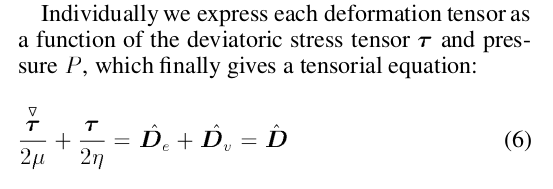
\includegraphics[width=8.25cm]{images/viscoelasticity/modm01c} \\
By taking the 'special' time derivative of the elastic equation we obtain  
\[
\frac{ \tilde{\bm \tau}}{2\mu} + \frac{{\bm \tau}}{2\eta}  
= \dot{\bm \varepsilon}_e^d + \dot{\bm \varepsilon}_v^d = \dot{\bm \varepsilon}^d 
\]
\end{multicols}

\newpage
\begin{multicols}{2}
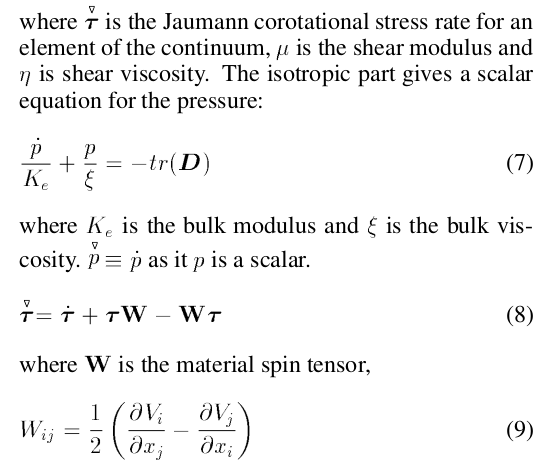
\includegraphics[width=8.25cm]{images/viscoelasticity/modm01d}\\
\[
\frac{\dot{p}}{K_e}+\frac{p}{\xi} = - {\rm tr} (\dot{\bm \varepsilon})
\]
\[
\tilde{\bm \tau} = \dot{\bm \tau} + {\bm \tau} \cdot \dot{\bm \omega} + \dot{\bm \omega} \cdot {\bm \tau}  
\]
\[
\dot{\bm \omega} = \frac12 (\vec\nabla \vec\upnu  - \vec\nabla \vec\upnu^T  ) 
\]

\end{multicols}

\begin{multicols}{2}
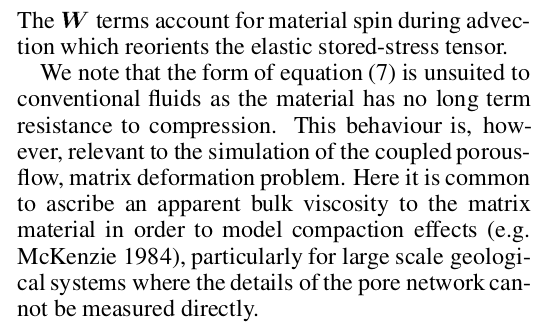
\includegraphics[width=8.25cm]{images/viscoelasticity/modm01e}\\
\end{multicols}

\begin{multicols}{2}
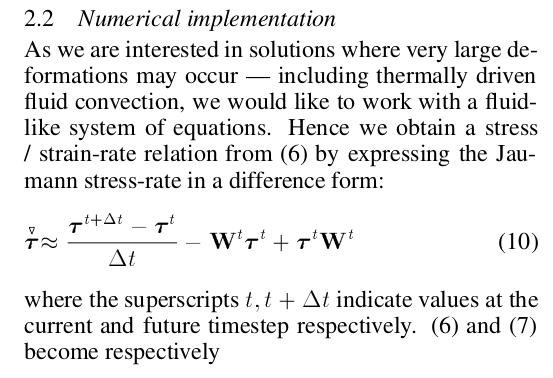
\includegraphics[width=8.25cm]{images/viscoelasticity/modm01f}\\
\[
\tilde{\bm \tau} = \frac{ {\bm \tau}^{t+\delta t} - {\bm \tau}^t }{\delta t} 
+ {\bm \tau}^t \cdot \dot{\bm \omega}^t + \dot{\bm \omega}^t \cdot {\bm \tau}^t  
\]

\end{multicols}

\begin{multicols}{2}
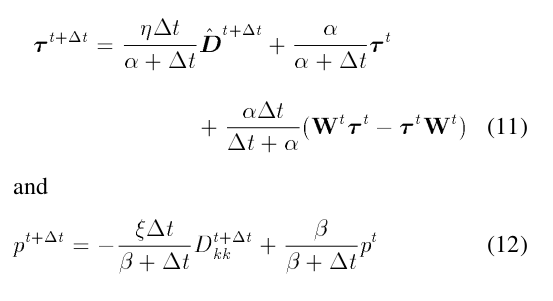
\includegraphics[width=8.25cm]{images/viscoelasticity/modm01g}\\
{\color{red} derive!!}
\[
{\bm \tau}^{t+\delta t} = \frac{\eta \delta t}{\eta/\mu + \delta t} {\bm \varepsilon}^{d,t+\delta t} + ...
\]
\[
p^{t + \delta t} = -\frac{\xi \delta t}{\xi/K_e + \delta_t } + \frac{}{} p^t
\]
\end{multicols}

\newpage
\begin{multicols}{2}
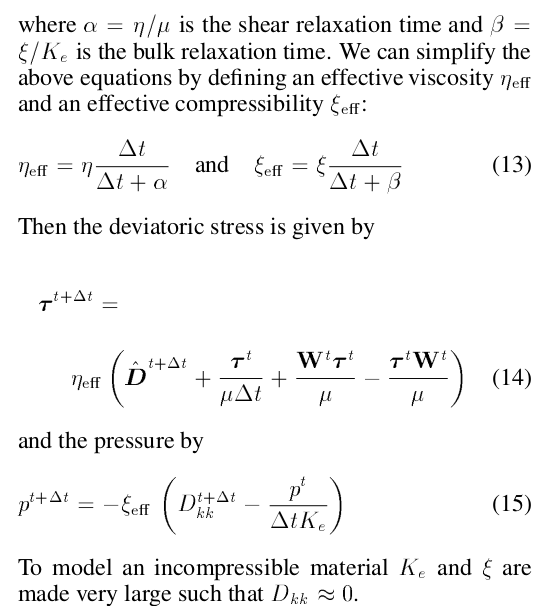
\includegraphics[width=8.25cm]{images/viscoelasticity/modm01h}\\
\end{multicols}

\begin{multicols}{2}
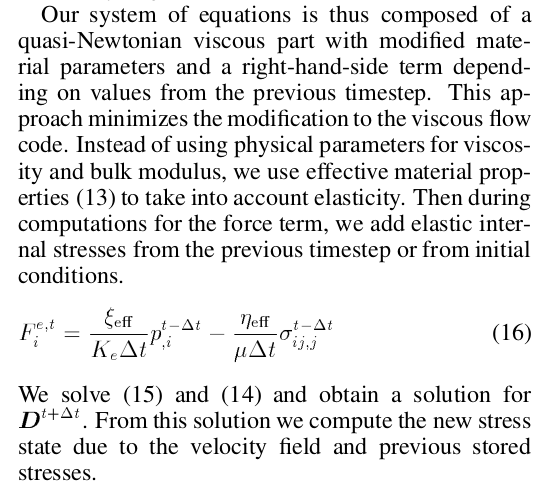
\includegraphics[width=8.25cm]{images/viscoelasticity/modm01i}\\
\end{multicols}

\begin{multicols}{2}
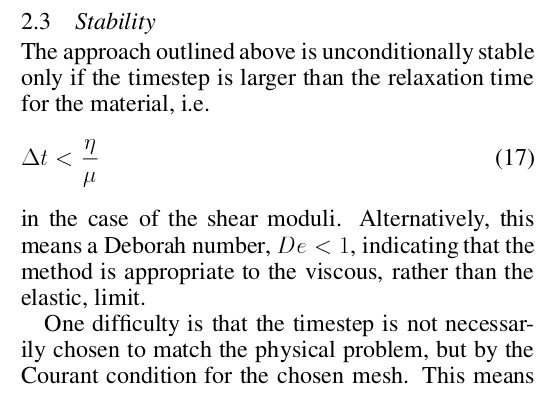
\includegraphics[width=8.25cm]{images/viscoelasticity/modm01j}\\
\end{multicols}

\begin{multicols}{2}
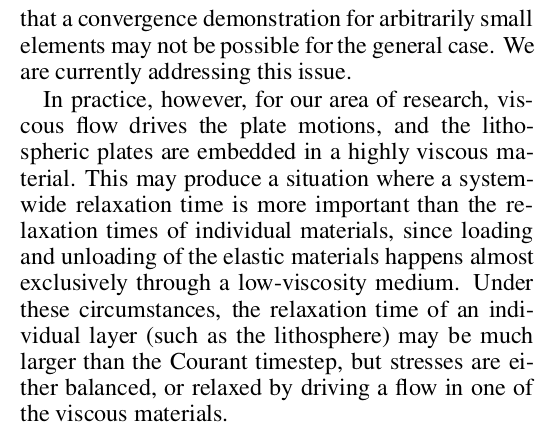
\includegraphics[width=8.25cm]{images/viscoelasticity/modm01k}\\
\end{multicols}

\begin{multicols}{2}
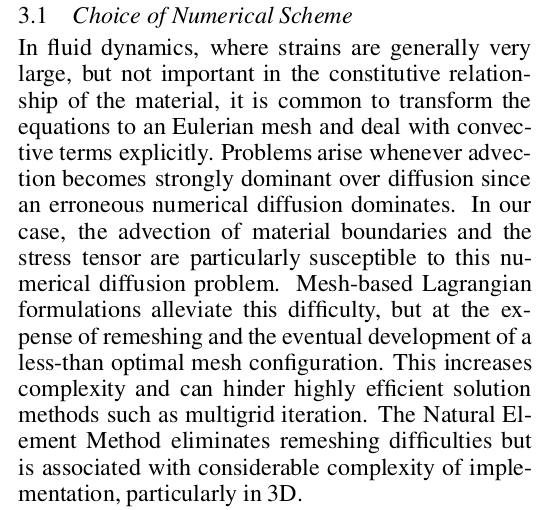
\includegraphics[width=8.25cm]{images/viscoelasticity/modm01l}\\
\end{multicols}

\begin{multicols}{2}
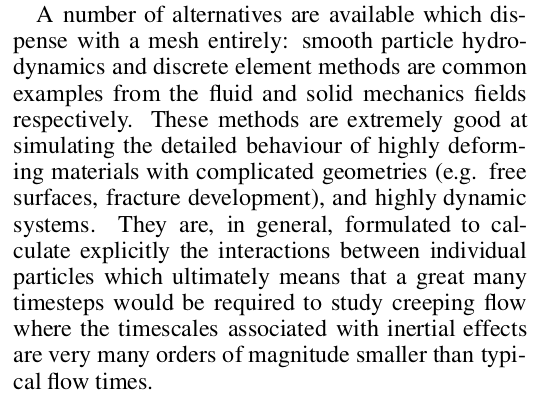
\includegraphics[width=8.25cm]{images/viscoelasticity/modm01m}\\
\end{multicols}

\newpage
\begin{multicols}{2}
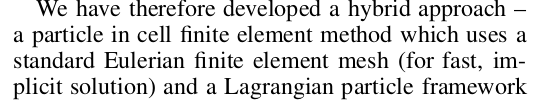
\includegraphics[width=8.25cm]{images/viscoelasticity/modm01n}
\end{multicols}

\begin{multicols}{2}
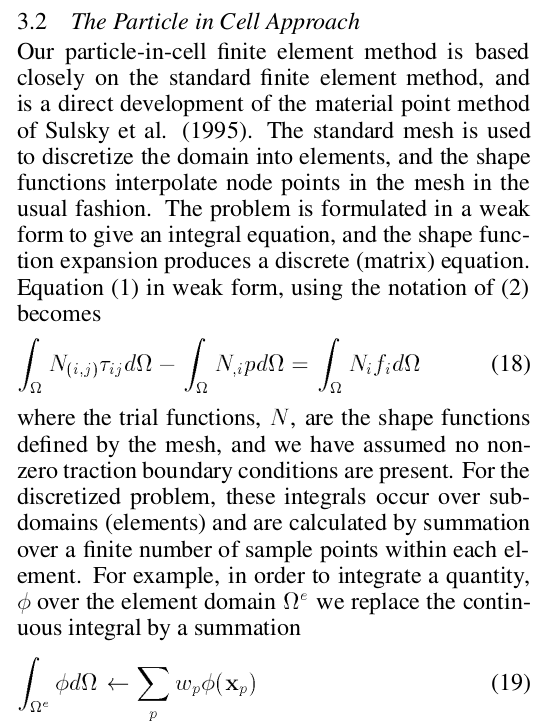
\includegraphics[width=8.25cm]{images/viscoelasticity/modm01p}\\
\end{multicols}

\begin{multicols}{2}
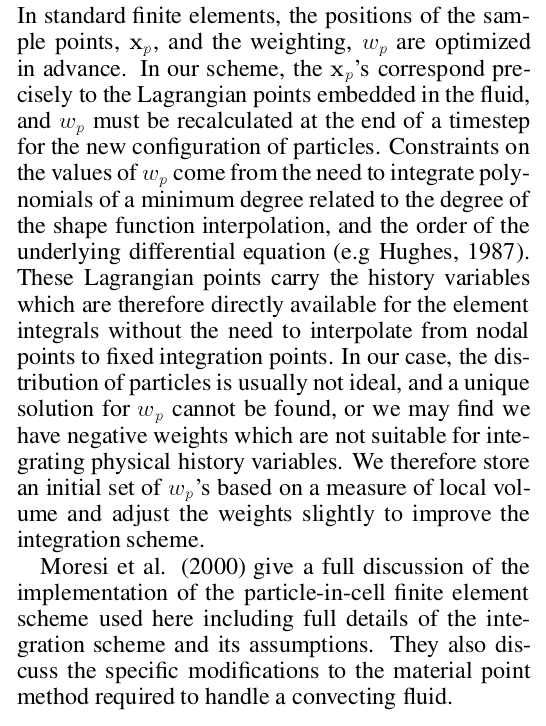
\includegraphics[width=8.25cm]{images/viscoelasticity/modm01q}\\
\end{multicols}





\newpage
\subsection{appendix: Equations in modm02\label{ve_modm02}} 
\fullcite{modm02}

%-------------------
\begin{multicols}{2}
\begin{center}
{\bf Article excerpts}
\\ 
{\bf Notes and remarks}
\end{center}
\end{multicols}

\begin{multicols}{2}
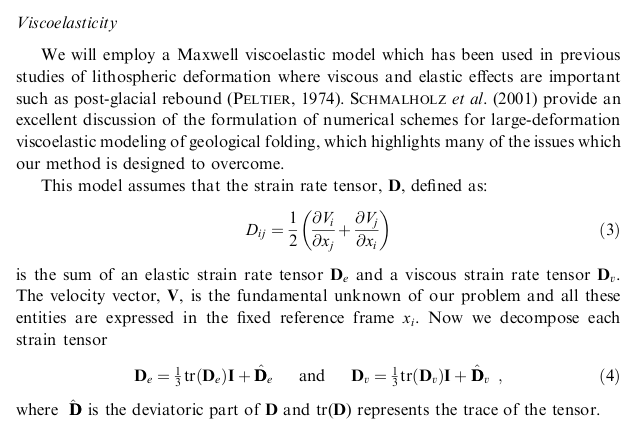
\includegraphics[width=8.25cm]{images/viscoelasticity/modm02a}\\
\[
\dot{\bm\varepsilon}=\frac12
(\vec\nabla \vec\upnu + \vec\nabla \vec\upnu ^T )
\]
\[
\dot{\bm\varepsilon}_e^d = 
\dot{\bm\varepsilon}_e  - \frac13 {\rm tr} (\dot{\bm\varepsilon}_e) {\bm 1} 
\]
\[
\dot{\bm\varepsilon}_v^d = 
\dot{\bm\varepsilon}_v  - \frac13 {\rm tr} (\dot{\bm\varepsilon}_v) {\bm 1} 
\]

\end{multicols}

\begin{multicols}{2}
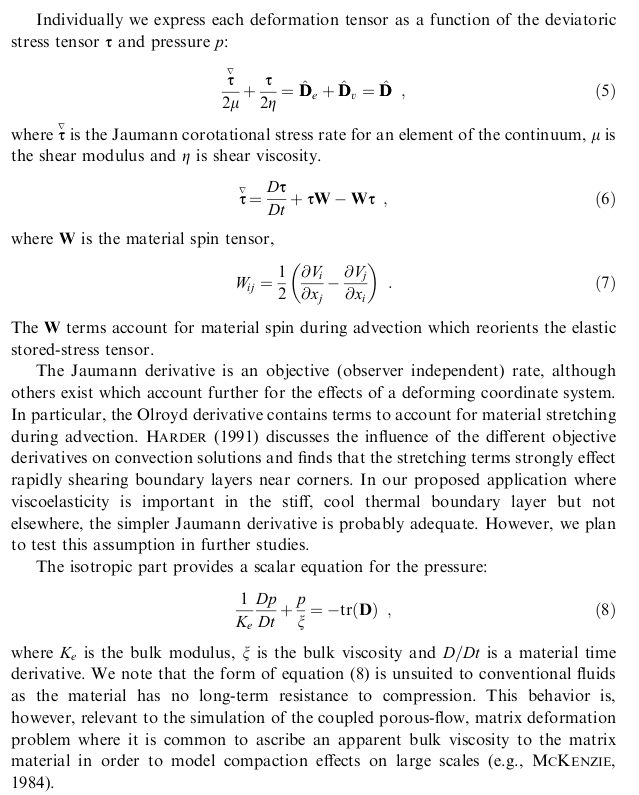
\includegraphics[width=8.25cm]{images/viscoelasticity/modm02b}\\
\[
\frac{TRIANGLE {\bm \tau}}{2 \mu}+\frac{{\bm \tau} }{2 \eta}
=
\dot{\bm\varepsilon}_e^d 
+
\dot{\bm\varepsilon}_v^d
=
\dot{\bm\varepsilon}^d 
\]
where 
$TRIANGLE {\bm \tau}$ is the Jaumann corotational stress rate
with 
\[
TRIANGLE {\bm \tau} = 
\frac{{\cal D}{\bm \tau}}{Dt} + 
{\bm\tau}\cdot {\bm\omega} - {\bm\omega}\cdot {\bm \tau}
\]


\[
\frac{1}{K} \frac{Dp}{Dt} + \frac{p}{\xi} = -{\rm tr}(\dot{\bm\varepsilon})
\]
\end{multicols}

\begin{multicols}{2}
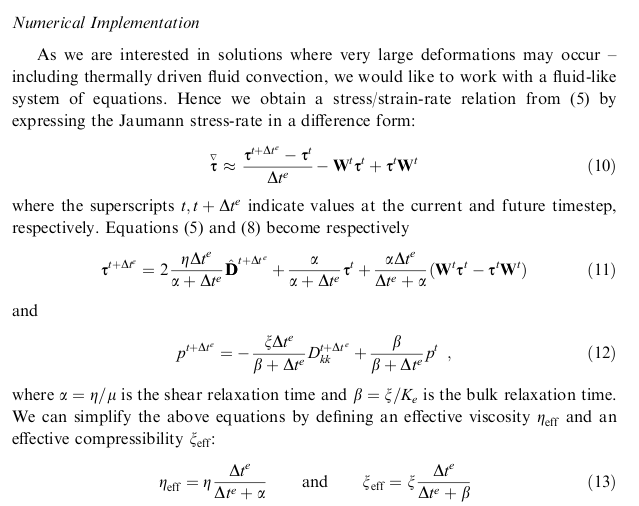
\includegraphics[width=8.25cm]{images/viscoelasticity/modm02c}\\
Numerical implementation
\[
TRIANGLE
\]
\end{multicols}

\begin{multicols}{2}
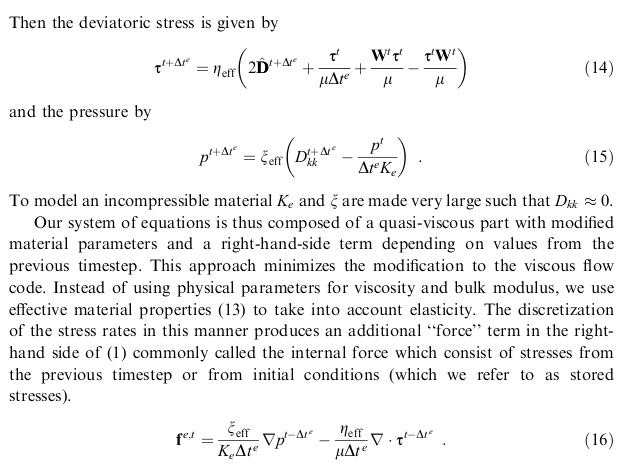
\includegraphics[width=8.25cm]{images/viscoelasticity/modm02d}\\
\end{multicols}

\begin{multicols}{2}
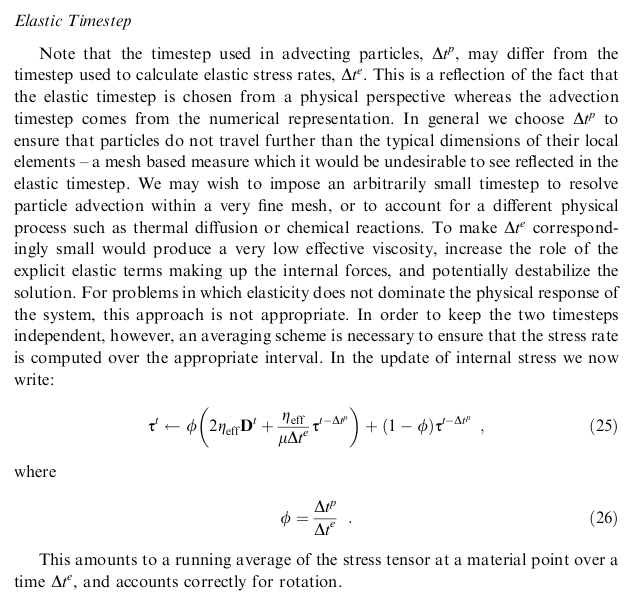
\includegraphics[width=8.25cm]{images/viscoelasticity/modm02e}\\
\end{multicols}

\begin{multicols}{2}
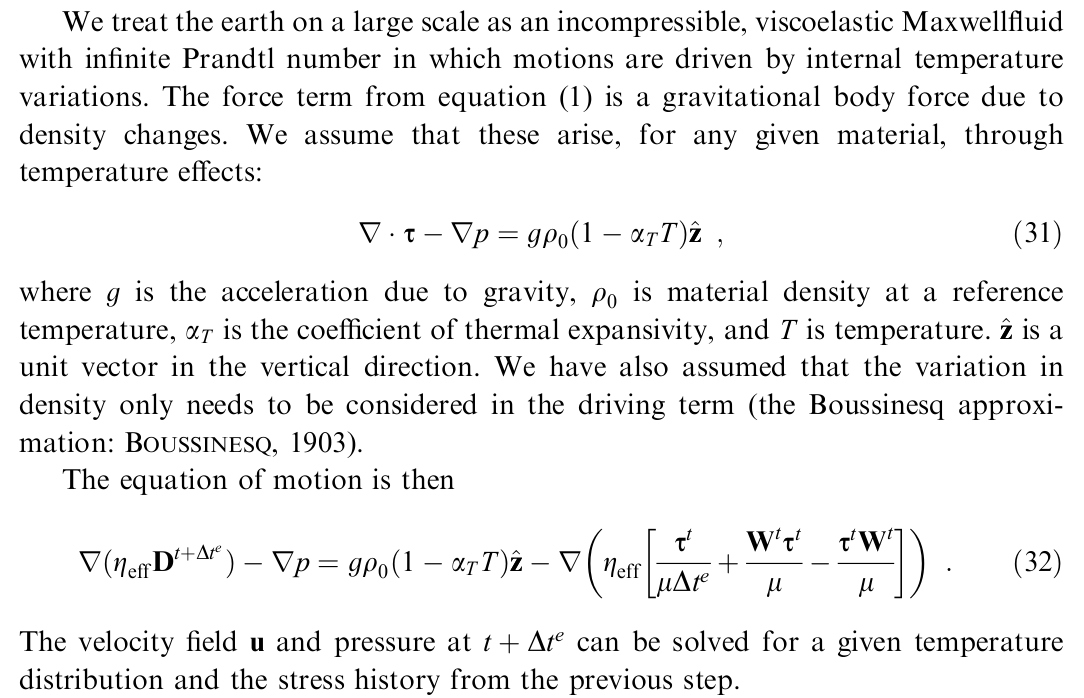
\includegraphics[width=8.25cm]{images/viscoelasticity/modm02h}\\
\end{multicols}









\newpage
\subsection{appendix: Equations in modm03\label{ve_modm03}} 
\fullcite{modm03}

Note that the paper also had a section about the implementation of plasticity.


\begin{multicols}{2}
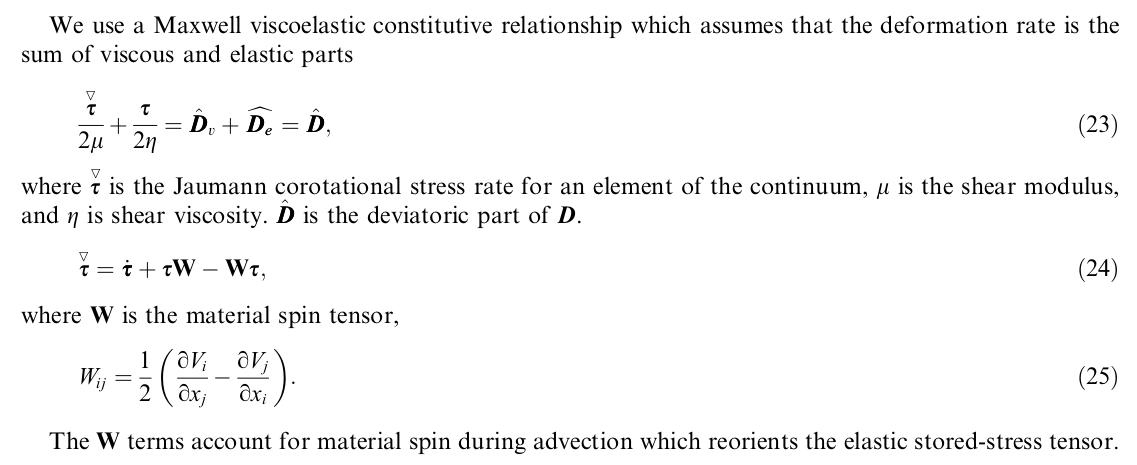
\includegraphics[width=8.25cm]{images/viscoelasticity/modm03a}
\end{multicols}

\begin{multicols}{2}
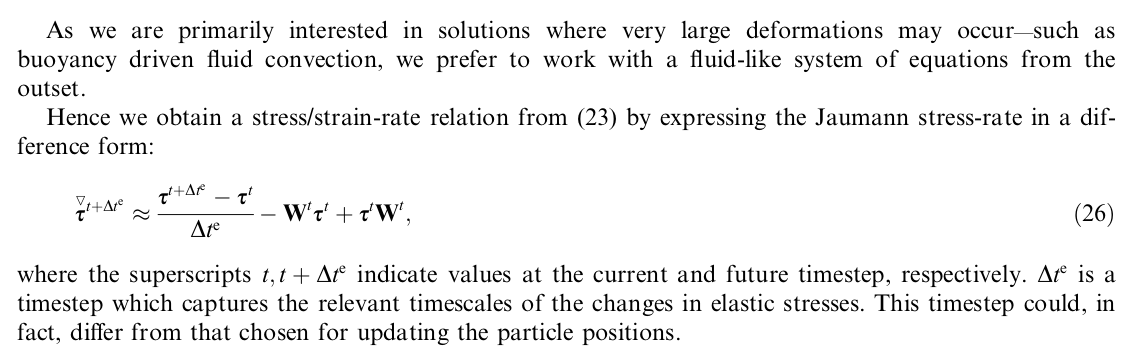
\includegraphics[width=8.25cm]{images/viscoelasticity/modm03b}\\
\[
\overset{\triangledown}{\bm \tau} = \dot{\bm \tau} 
+ {\bm \tau} \cdot \dot{\bm\omega} - \dot{\bm\omega} \cdot {\bm \tau}
\]
\end{multicols}

\begin{multicols}{2}
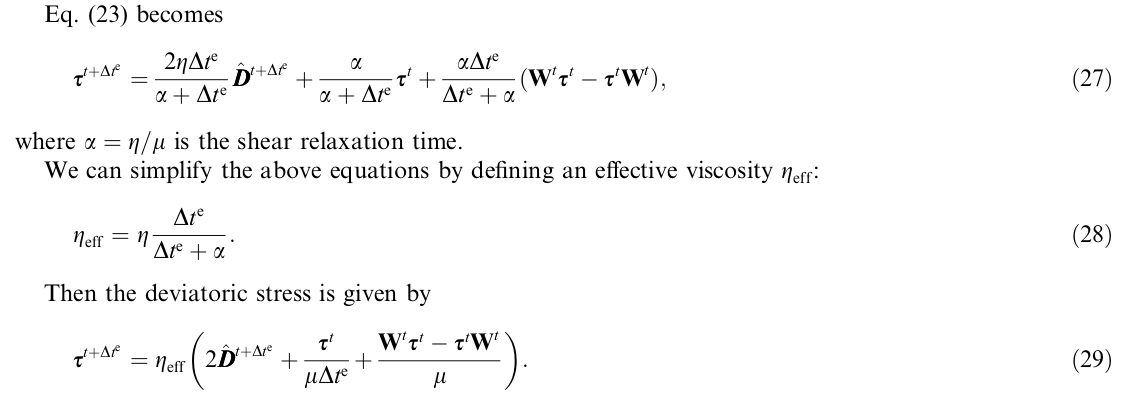
\includegraphics[width=8.25cm]{images/viscoelasticity/modm03c}
\end{multicols}

\begin{multicols}{2}
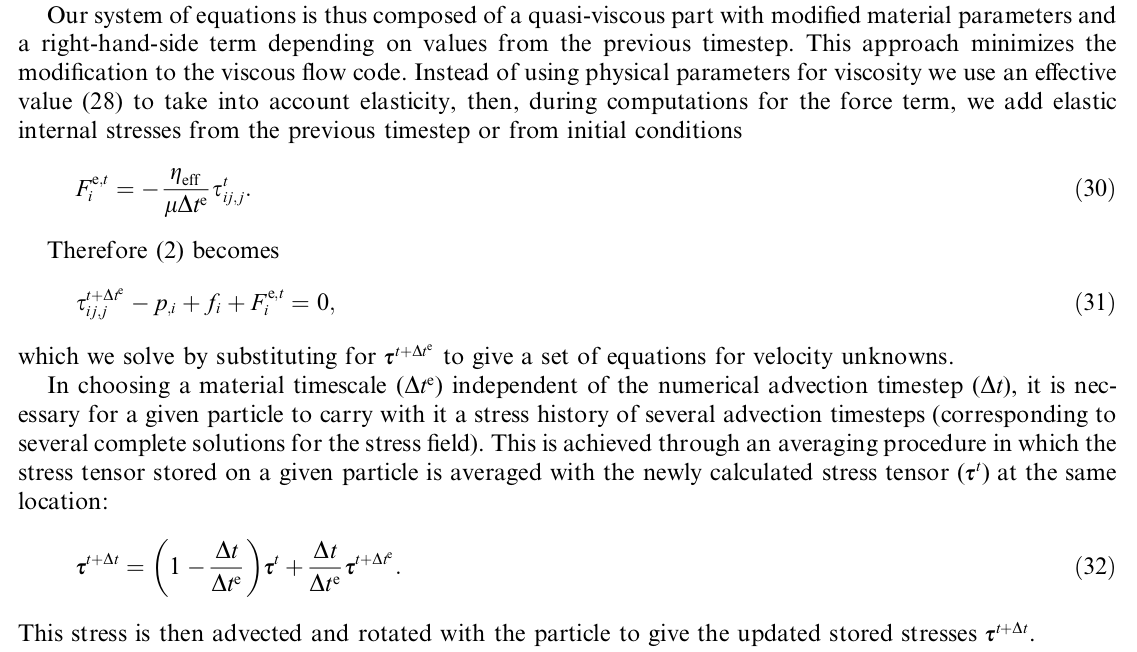
\includegraphics[width=8.25cm]{images/viscoelasticity/modm03d}
\end{multicols}






\newpage
\subsection{appendix: Equations in mure05\label{ve_mure05}} 
\fullcite{mure05}

%..............................
\paragraph{Constitutive models}.

\begin{multicols}{2}
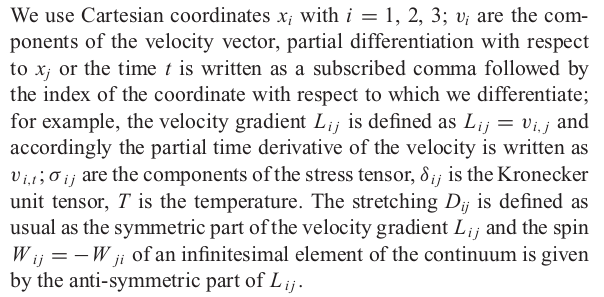
\includegraphics[width=8cm]{images/viscoelasticity/mure05a}\\
\end{multicols}

\begin{multicols}{2}
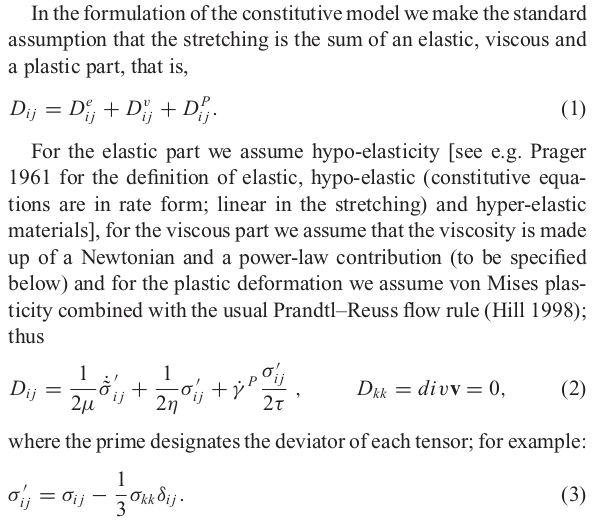
\includegraphics[width=8cm]{images/viscoelasticity/mure05b}\\
\[
\dot{\bm\varepsilon} = 
\dot{\bm\varepsilon}^e +
\dot{\bm\varepsilon}^v +
\dot{\bm\varepsilon}^p 
\]
\[
\dot{\bm\varepsilon}=\frac{1}{2\mu} \frac{{\cal D}{\bm\tau}}{{\cal D}t} 
+ \frac{1}{2\eta} {\bm \tau} + \dot{\gamma}^p \frac{{\bm \tau}}{\tau_e}
\]
\[
{\rm tr}(\dot{\bm\varepsilon} = {\rm div}(\vec\upnu)= 0 
\]
\end{multicols}

\begin{multicols}{2}
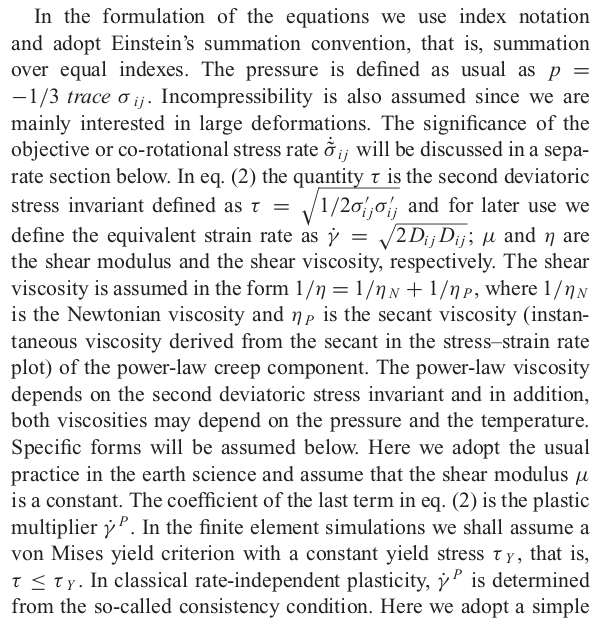
\includegraphics[width=8cm]{images/viscoelasticity/mure05c}\\
\[
p=-\frac13 {\rm tr}({\bm\sigma})
\]
\end{multicols}

\begin{multicols}{2}
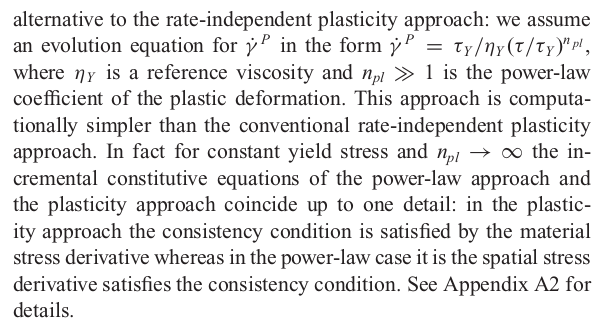
\includegraphics[width=8cm]{images/viscoelasticity/mure05d}\\
\[
\dot\gamma= \frac{\tau_y}{\eta_y} \left(\frac{\tau_e}{\tau_y}\right) ^{n_{pl}} 
\]
where $\eta_y$ is a reference viscosity and $n_{pl}>>1$ is the 
power-law coefficient of the plastic deformation.
\end{multicols}

\begin{multicols}{2}
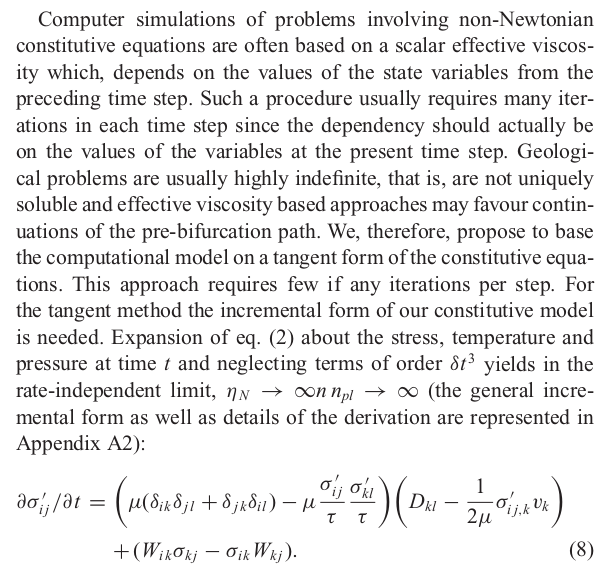
\includegraphics[width=8cm]{images/viscoelasticity/mure05e}\\
\[
 = ... \dot{\bm\omega}\cdot {\bm\sigma} - {\bm\sigma}\cdot \dot{\bm\omega}
\]
whaaat ??!?
\end{multicols}

\begin{multicols}{2}
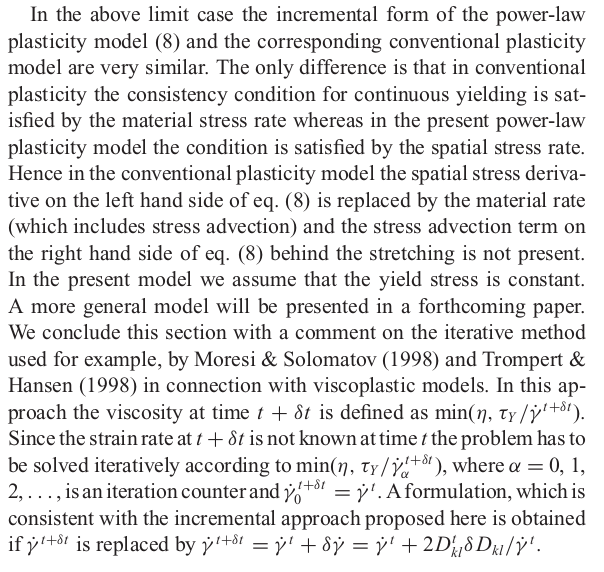
\includegraphics[width=8cm]{images/viscoelasticity/mure05f}\\
\end{multicols}

\newpage
%..................................
\paragraph{Objective stress rates}.

\begin{multicols}{2}
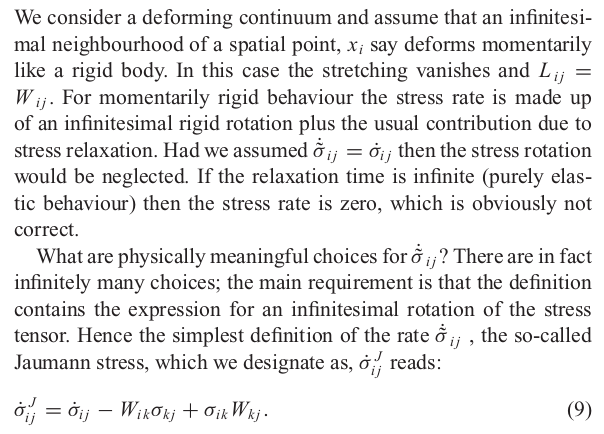
\includegraphics[width=8cm]{images/viscoelasticity/mure05g}\\
\end{multicols}

\begin{multicols}{2}
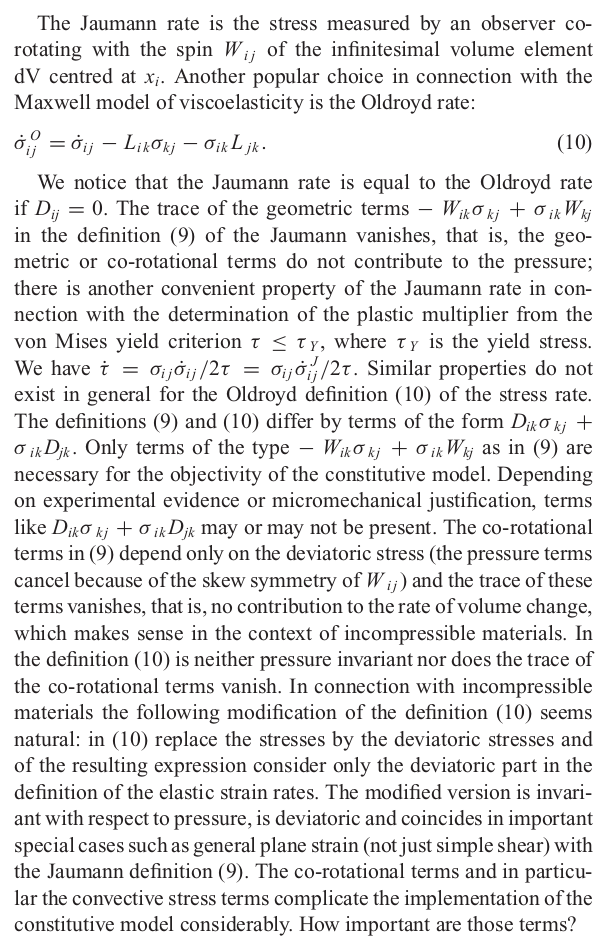
\includegraphics[width=8cm]{images/viscoelasticity/mure05h}\\
\end{multicols}

\begin{multicols}{2}
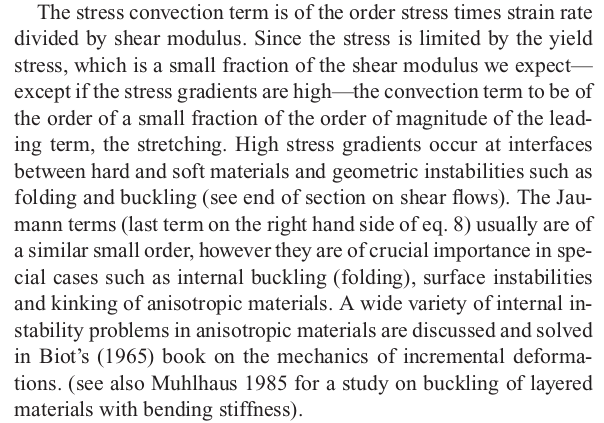
\includegraphics[width=8cm]{images/viscoelasticity/mure05i}\\
\end{multicols}

\begin{multicols}{2}
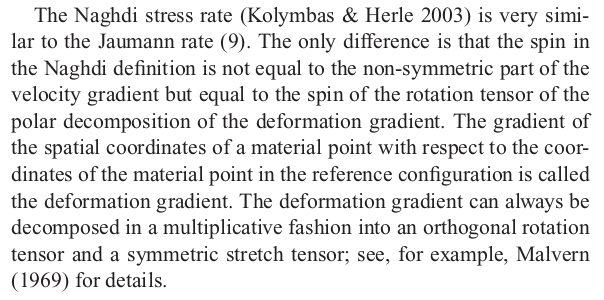
\includegraphics[width=8cm]{images/viscoelasticity/mure05j}\\
\end{multicols}

\begin{multicols}{2}
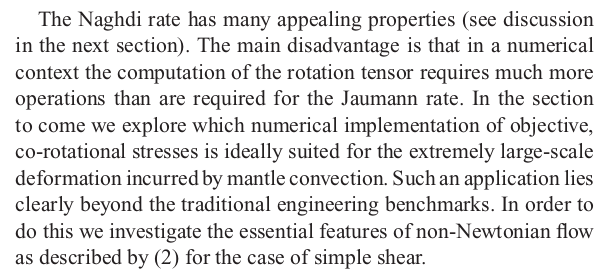
\includegraphics[width=8cm]{images/viscoelasticity/mure05k}\\
\end{multicols}








\newpage
\subsection{appendix: Equations in kabe07\label{ve_kabe07}} 
\fullcite{kabe07}

\begin{multicols}{2}
\begin{center}
{\bf Article excerpts}
\\ 
{\bf Notes and remarks}
\end{center}
\end{multicols}

%------------------------------------------------------------------------------

\begin{multicols}{2}
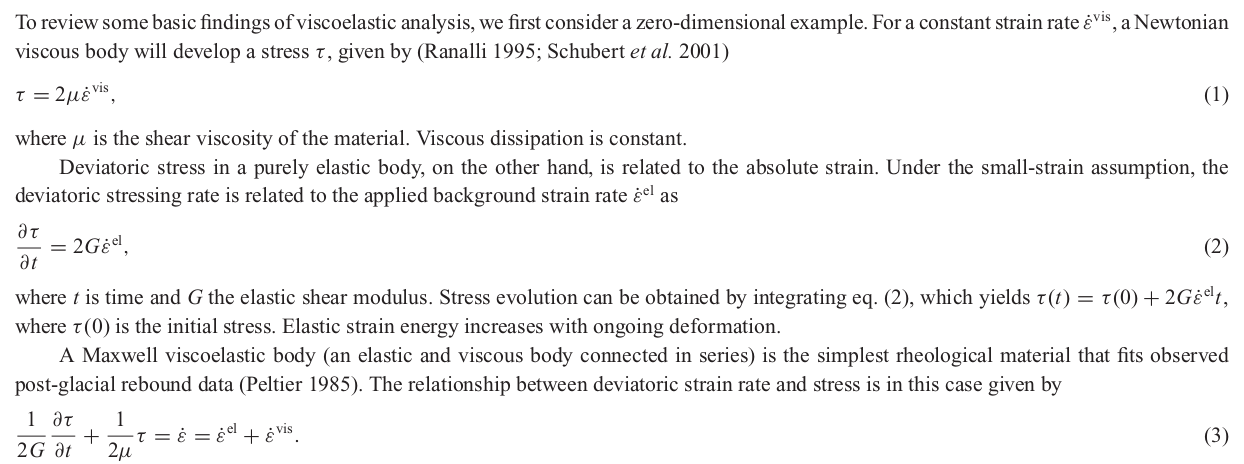
\includegraphics[width=8.4cm]{images/viscoelasticity/kabe07_a}\\
\end{multicols}

\begin{multicols}{2}
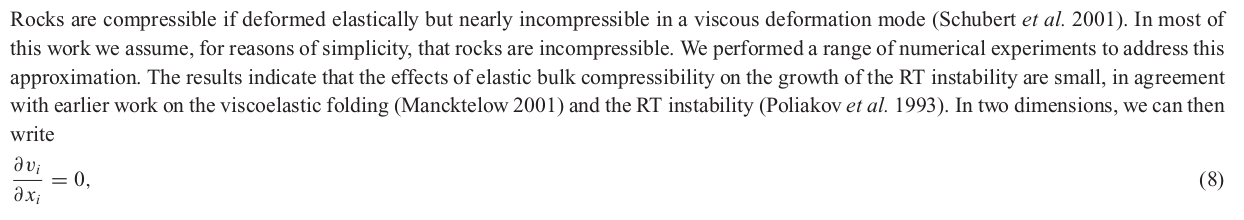
\includegraphics[width=8.4cm]{images/viscoelasticity/kabe07_b}\\
\end{multicols}

\begin{multicols}{2}
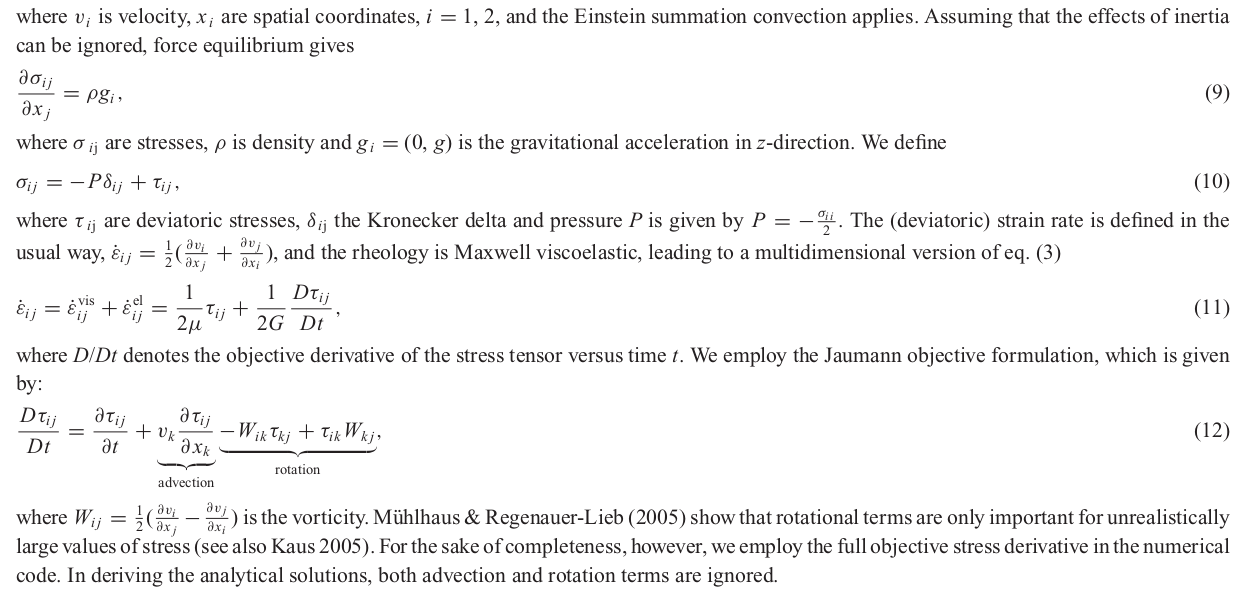
\includegraphics[width=8.4cm]{images/viscoelasticity/kabe07_c}\\
\end{multicols}


\newpage
\subsection{appendix: Equations in moql07\label{ve_moql07}} 
\fullcite{moql07}

\begin{multicols}{2}
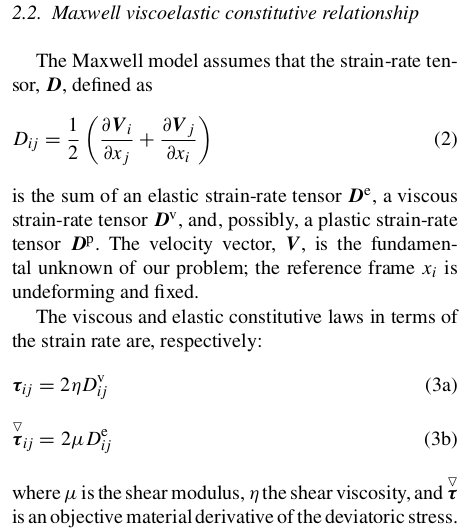
\includegraphics[width=8.25cm]{images/viscoelasticity/moql07a}\\
\[
\dot{\bm\varepsilon}=\frac12
(\vec\nabla \vec\upnu + \vec\nabla \vec\upnu ^T )
\]
\[
{\bm \tau}=2\eta \dot{\bm\varepsilon}^v
\]
\[
\tilde{\bm \tau}=2\mu \dot{\bm\varepsilon}^e
\]
\end{multicols}

\begin{multicols}{2}
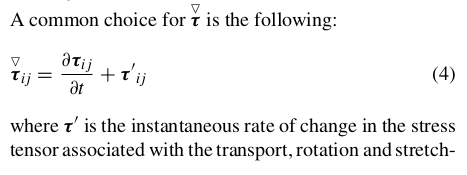
\includegraphics[width=8.25cm]{images/viscoelasticity/moql07b}\\
\[
\tilde{\bm \tau} = \frac{\partial {\bm \tau}}{\partial t}
+ (\vec\upnu\cdot \vec\nabla) {\bm \tau} 
+ {\bm \tau}\cdot \dot{\bm\omega} - \dot{\bm\omega}\cdot {\bm \tau}
+ a ( {\bm \tau} \cdot \dot{\bm\varepsilon} +  \dot{\bm\varepsilon} \cdot {\bm \tau} )
\]
with $-1 \le a \le 1$.
\end{multicols}

\begin{multicols}{2}
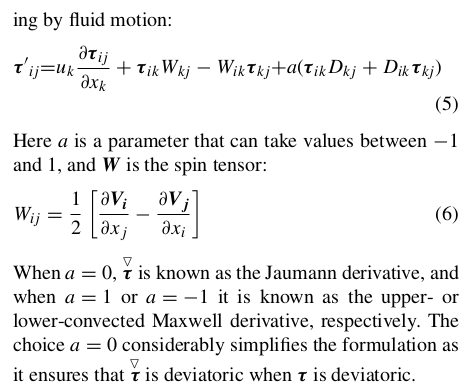
\includegraphics[width=8.25cm]{images/viscoelasticity/moql07c}\\
\[
\dot{\bm\varepsilon} = \dot{\bm\varepsilon}^e+ \dot{\bm\varepsilon}^v
= \frac{\tilde{\bm \tau}}{2\mu} + \frac{{\bm \tau}}{2\eta}
\]
\end{multicols}

\newpage
\begin{multicols}{2}
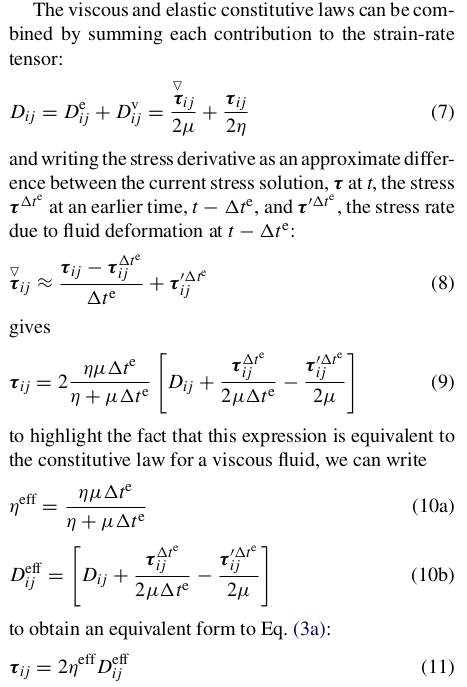
\includegraphics[width=8.25cm]{images/viscoelasticity/moql07d} \\
\[
\dot{\bm\varepsilon} 
= \dot{\bm\varepsilon}^e + \dot{\bm\varepsilon}^v 
= \frac{\tilde{\bm \tau}  }{2\mu} + \frac{ {\bm \tau}}{2\eta}
\]

\[
\tilde{\bm \tau}^{k+1} \simeq \frac{ {\bm\tau}^{k+1}-{\bm\tau}^k }{\delta t} + \underline{\bm\tau}^k
\]

\[
{\bm\tau} = 2 \frac{\eta \mu \delta t}{\eta + \mu  \delta t}
\left(
\dot{\bm\varepsilon}  + \frac{{\bm\tau}^k}{2\mu \delta t} - \frac{\underline{\bm\tau}^k}{2\mu}
\right)
\]

\[
\eta_{ve} = \frac{\eta \mu \delta t}{\eta + \mu  \delta t}
\]

\end{multicols}


\newpage
\subsection{appendix: Equations in bepo10\label{ve_bepo10}} 
\fullcite{bepo10}

This is in my opinion a fantastic article. 
Physics is explained, FEM discretisation is derived, 
with benchmarks and experiments.


\fbox{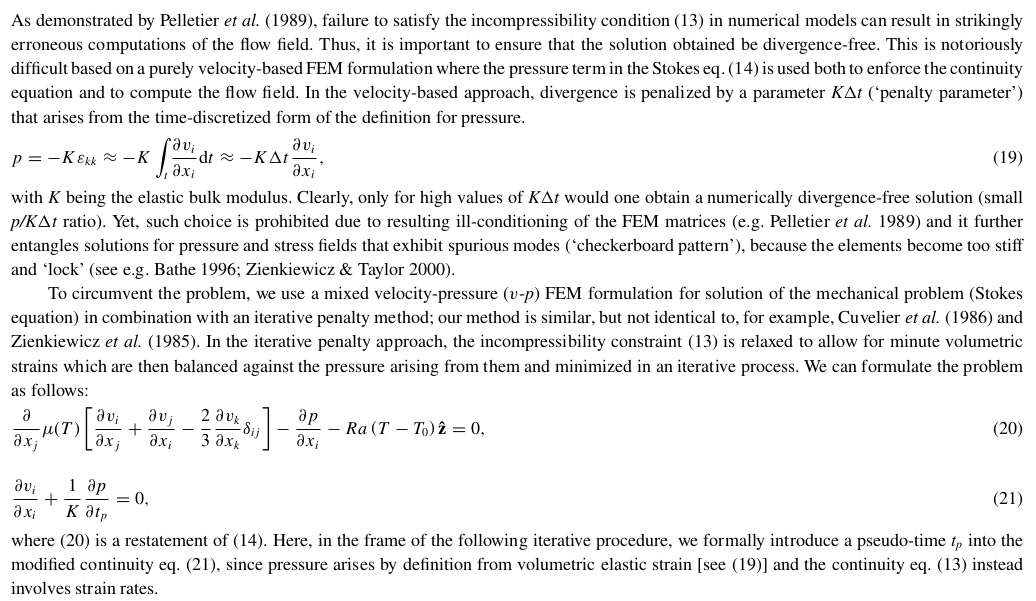
\includegraphics[width=15cm]{images/viscoelasticity/bepo10_a}}

\[
p=-K \varepsilon_{kk} = -K {\rm tr}({\bm \varepsilon})
\]
\[
\vec\nabla\cdot\vec\upnu + \frac{1}{K} \frac{\partial p}{\partial t_p} = 0
\]

\fbox{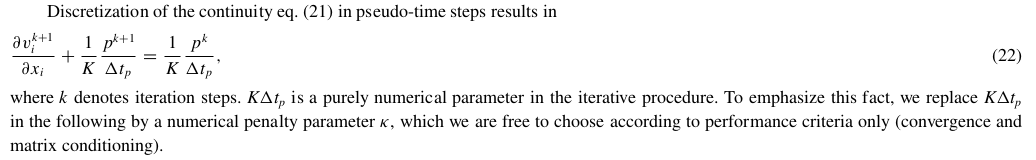
\includegraphics[width=15cm]{images/viscoelasticity/bepo10_ba}}
\[
\vec\nabla\cdot\vec\upnu^{k+1} + \frac{1}{K} \frac{p^{k+1}}{\delta t_p}  = \frac{1}{K} \frac{p^{k}}{\delta t_p}
\Rightarrow
\vec\nabla\cdot\vec\upnu^{k+1} + \frac{1}{\kappa} p^{k+1}  = \frac{1}{\kappa} p^{k}
\]

\fbox{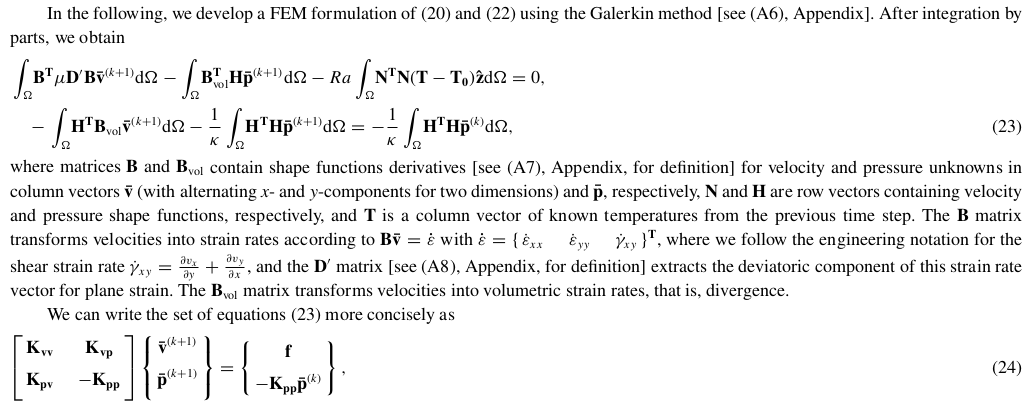
\includegraphics[width=15cm]{images/viscoelasticity/bepo10_bb}}

\fbox{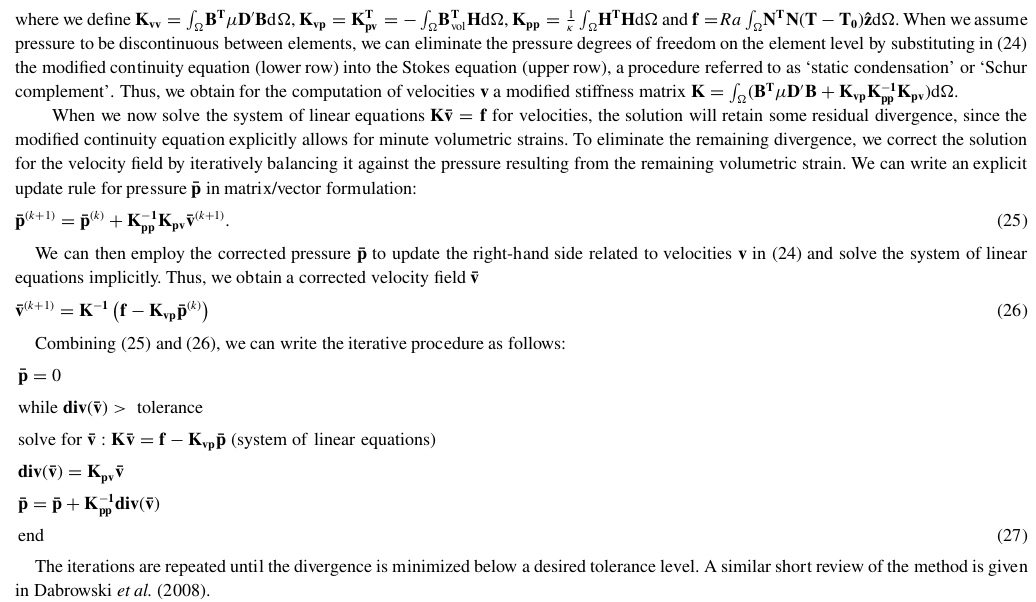
\includegraphics[width=15cm]{images/viscoelasticity/bepo10_c}}

\vspace{.5cm}

``
Use of a viscous rheology might be appropriate for modelling the dynamics of the hot, 
convecting interior of our planet. Yet, when the relatively cold, elastic lithosphere 
is included in the simulation, a viscoelastic rheology is more appropriate. While the 
hot, sublithospheric interior experiences strong deformation on geological timescales 
and thus behaves like a viscous fluid, the lithosphere itself remains relatively
undeformed over long geological times and exhibits the properties of an elastic solid. 
The difference in response of the mantle in the relatively hot sublithospheric interior 
and the relatively cold lithosphere is a consequence of the strong temperature dependence 
of creep activation in mantle rocks (Karato \& Wu 1993). A Maxwell rheology naturally 
combines both viscous and elastic behaviour of mantle rocks, with the transition between 
the two rheological regimes being determined by the temperature-dependent viscosity and 
the timescale considered.
''

\vspace{.5cm}

\fbox{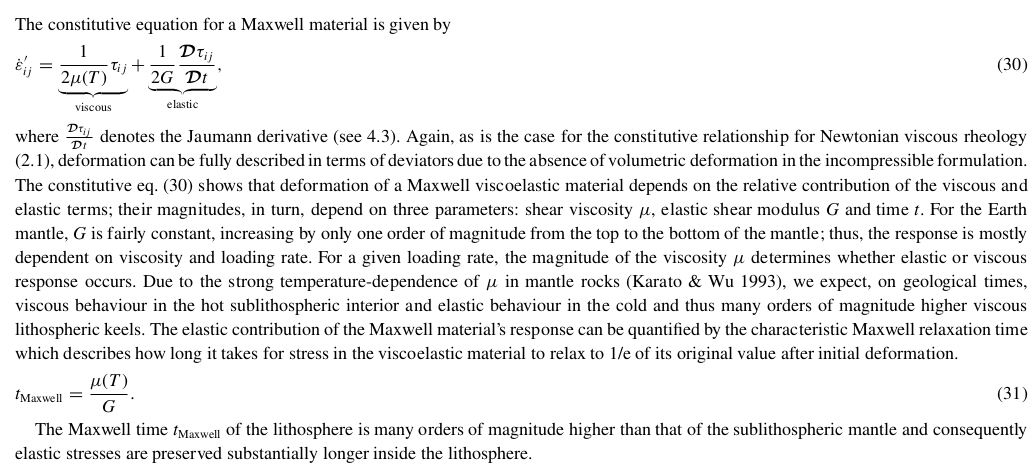
\includegraphics[width=15cm]{images/viscoelasticity/bepo10_d}}



\fbox{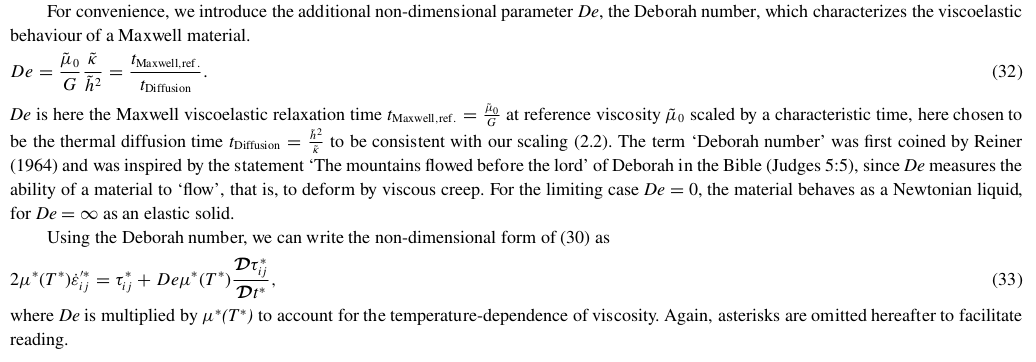
\includegraphics[width=15cm]{images/viscoelasticity/bepo10_e}}

\fbox{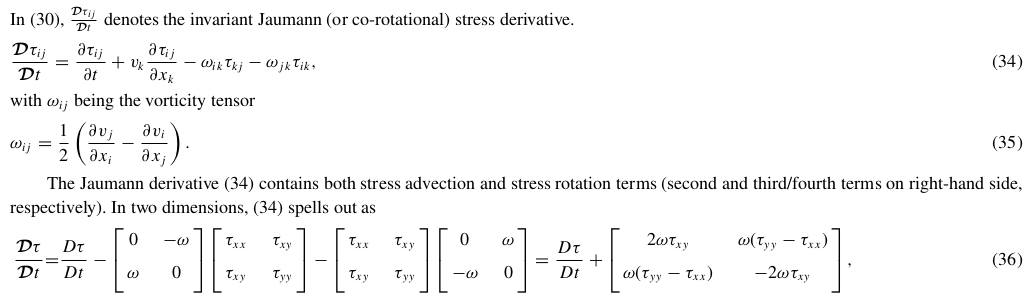
\includegraphics[width=15cm]{images/viscoelasticity/bepo10_f}}

\fbox{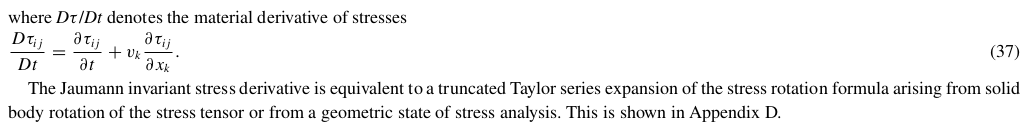
\includegraphics[width=15cm]{images/viscoelasticity/bepo10_g}}


\paragraph{Derivation of Jaumann derivative from stress rotation formula}.

\fbox{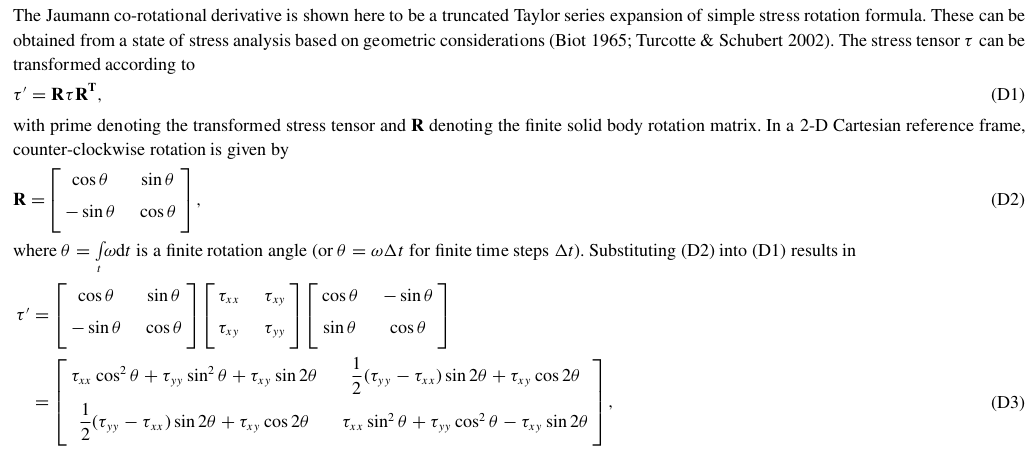
\includegraphics[width=15cm]{images/viscoelasticity/bepo10_h}}\\
\[
{\bm \tau}' = {\bm R} \cdot {\bm \tau} \cdot {\bm R}^T
\]
\[
{\bm R} = 
\left(\begin{array}{cc}
\cos\theta & \sin\theta \\
-\sin\theta  & \cos\theta
\end{array}\right)
\]
\[
\theta = \int_t \omega \; dt \simeq \omega \delta t
\]
\[
{\bm \tau}' = 
\left(\begin{array}{cc}
\cos\theta & \sin\theta \\
-\sin\theta  & \cos\theta
\end{array}\right)
\cdot
\left(\begin{array}{cc}
\tau_{xx} & \tau_{xy} \\
\tau_{xy} & \tau_{yy}
\end{array}\right)
\cdot
\left(\begin{array}{cc}
\cos\theta & -\sin\theta \\
\sin\theta & \cos\theta
\end{array}\right)
\]

\fbox{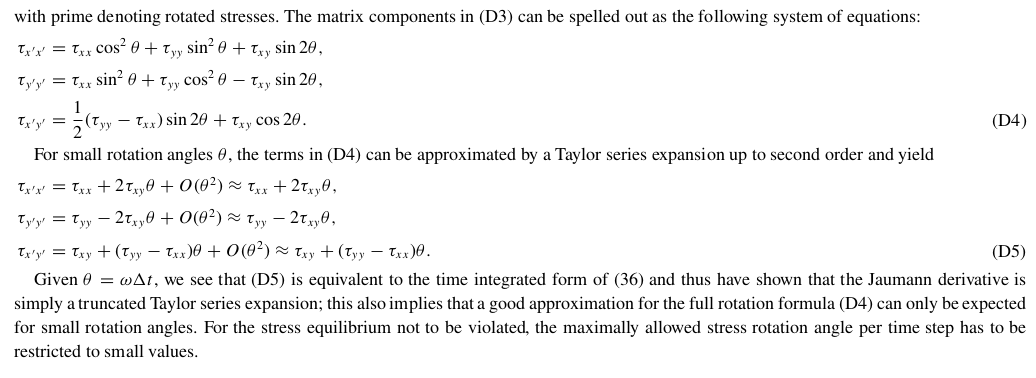
\includegraphics[width=15cm]{images/viscoelasticity/bepo10_i}}

\begin{eqnarray}
\tau_{xx}' &=& \tau_{xx} \cos^2 \theta  + \tau_{yy} \sin^2 \theta  + \tau_{xy} \sin 2 \theta\nn\\
\tau_{yy}' &=& \tau_{xx} \sin^2 \theta  + \tau_{yy} \cos^2 \theta  - \tau_{xy} \sin 2 \theta\nn\\
\tau_{xy}' &=& \frac12 (\tau_{yy}-\tau_{xx}) \sin 2\theta  + \tau_{xy} \cos 2\theta \nn
\end{eqnarray}


\begin{eqnarray}
\tau_{xx}' &=& \tau_{xx}  + 2\tau_{xy} \theta + {\cal O}(\theta^2) \simeq \tau_{xx} + 2\tau_{xy} \theta \nn\\
\tau_{yy}' &=& \tau_{yy}  - 2\tau_{xy} \theta + {\cal O}(\theta^2) \simeq \tau_{yy} - 2\tau_{xy} \theta \nn\\
\tau_{xy}' &=& \tau_{xy} + (\tau_{yy}-\tau_{xx}) \theta  + {\cal O}(\theta^2) \simeq \tau_{xy} + (\tau_{yy}-\tau_{xx}) \theta \nn
\end{eqnarray}

\paragraph{FEM implementation}.

\fbox{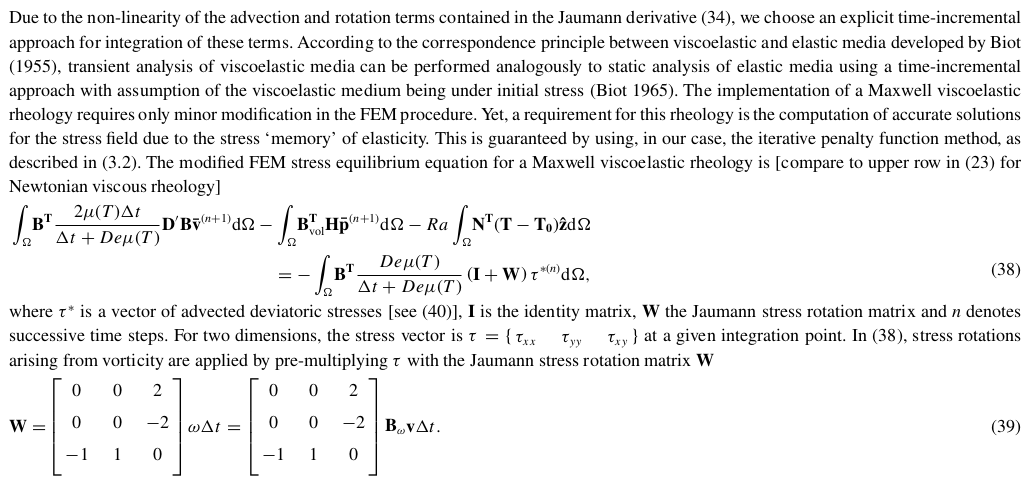
\includegraphics[width=15cm]{images/viscoelasticity/bepo10_j}}

\vspace{4cm}

\fbox{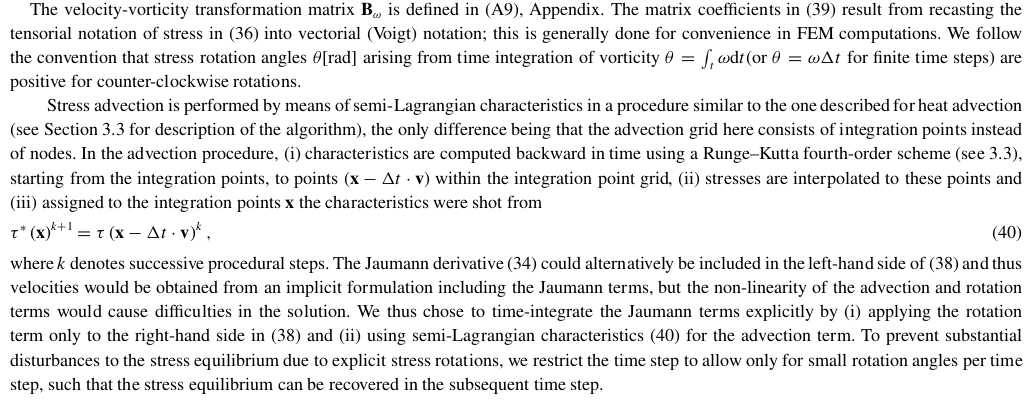
\includegraphics[width=15cm]{images/viscoelasticity/bepo10_k}}






\newpage
\subsection{appendix: Equations in beps10\label{ve_beps10}} 
\fullcite{beps10}

\begin{multicols}{2}
\begin{center}
{\bf Article excerpts}
\\ 
{\bf Notes and remarks}
\end{center}
\end{multicols}

%------------------------------------------------------------------------------

\begin{multicols}{2}
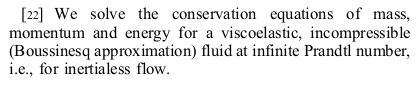
\includegraphics[width=8.3cm]{images/viscoelasticity/beps10a}
\end{multicols}

\begin{multicols}{2}
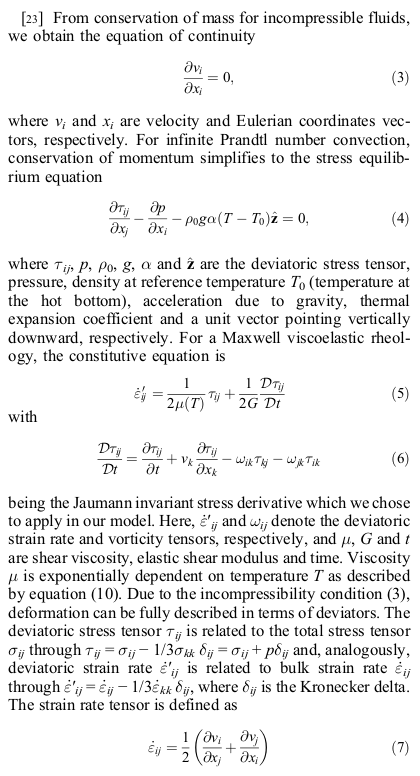
\includegraphics[width=8.3cm]{images/viscoelasticity/beps10b}\\
\[
\dot\varepsilon_{ij}^d = \frac{1}{2\eta} \tau_{ij} + \frac{1}{2\mu} \frac{{\cal D}\tau_{ij}}{{\cal D}t}
\]
with
\[
\frac{{\cal D}\tau_{ij}}{{\cal D}t} =  \frac{\partial \tau_{ij}}{\partial t} 
+ \upnu_k \frac{\partial \tau_{ij}}{\partial x_k}
- (\dot{\omega}_{ik}\tau_{kj} - \tau_{jk} \dot{\omega}_{ik} ) 
\]
\end{multicols}

\begin{multicols}{2}
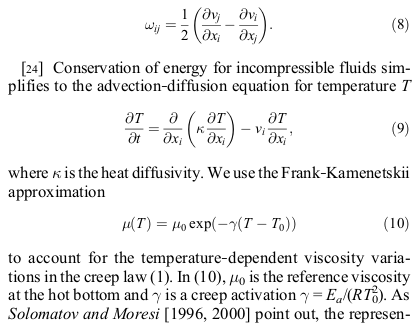
\includegraphics[width=8.3cm]{images/viscoelasticity/beps10c}
\end{multicols}





\newpage
\subsection{appendix: Equations in zhym12\label{ve_zhym12}} 
\fullcite{zhym12}


\begin{multicols}{2}
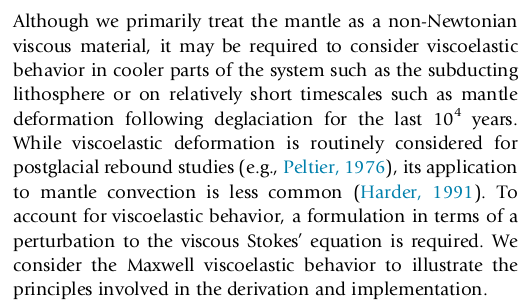
\includegraphics[width=8.25cm]{images/viscoelasticity/zhym12_a}
\end{multicols}

\begin{multicols}{2}
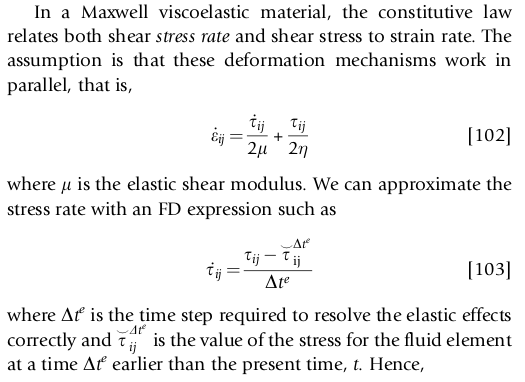
\includegraphics[width=8.25cm]{images/viscoelasticity/zhym12_b}\\
\[
\dot{\bm\varepsilon} = \frac{ \dot{\bm \tau}  }{2\mu} + \frac{{\bm \tau}}{2\eta} 
\]
\end{multicols}

\begin{multicols}{2}
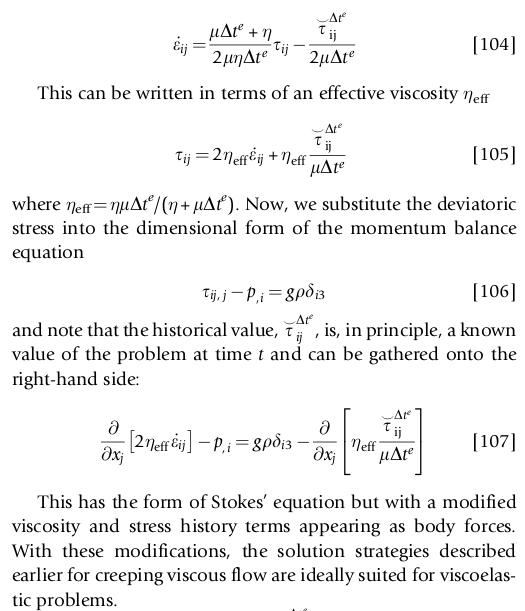
\includegraphics[width=8.25cm]{images/viscoelasticity/zhym12_c}\\
\[
\dot{\bm\varepsilon} = \frac{\mu \delta t^e + \eta}{2 \mu \eta \delta t^e} {\bm \tau}
- ... 
\]
\[
{\bm \tau} = 2 \eta_{ve} \dot{\bm\varepsilon} + \frac{\eta_{ve} {\bm \tau}^{before} }{\mu \delta t^e}
\]
\[
\eta_{ve}=\frac{\eta\mu \delta t^e}{\eta + \mu \delta t^e}
\]
\[
\vec\nabla \cdot (2 \eta_{ve} \dot{\bm\varepsilon}) - \vec\nabla p
=
\rho \vec{g}
-\vec\nabla \cdot(\eta_{ve}\frac{1}{\mu \delta t^e} ... )
\]
\end{multicols}

\begin{multicols}{2}
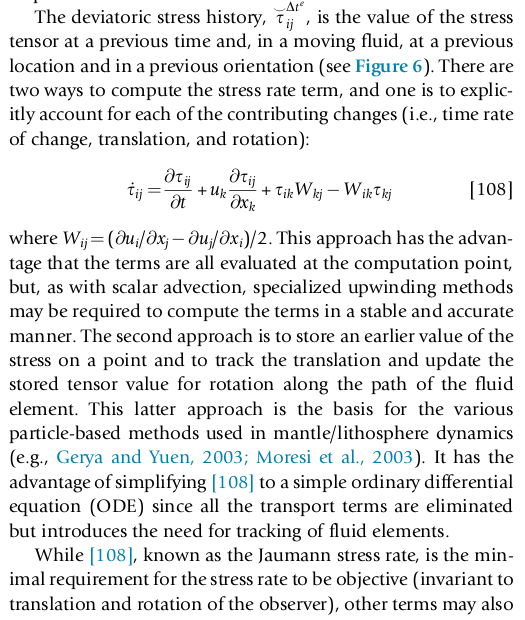
\includegraphics[width=8.25cm]{images/viscoelasticity/zhym12_d} \\
\[
{\bm \tau} = \frac{\partial {\bm \tau}}{\partial t} + 
(\vec\upnu \cdot \vec\nabla ){\bm \tau} + 
{\bm \tau} \cdot \dot{\bm\omega} - \dot{\bm\omega} \cdot {\bm\tau}
\]
\end{multicols}

\begin{multicols}{2}
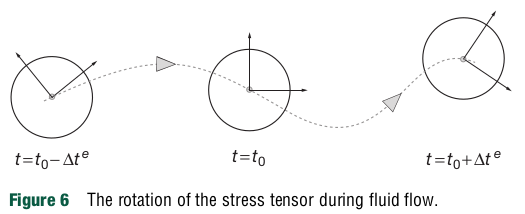
\includegraphics[width=8.25cm]{images/viscoelasticity/zhym12_e}
\end{multicols}

\begin{multicols}{2}
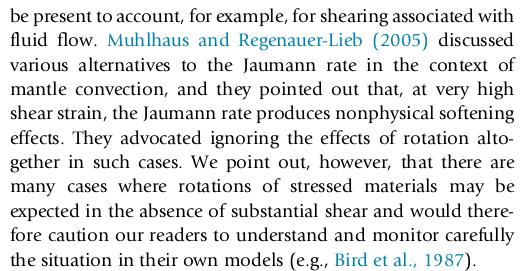
\includegraphics[width=8.25cm]{images/viscoelasticity/zhym12_f}
\end{multicols}

\begin{multicols}{2}
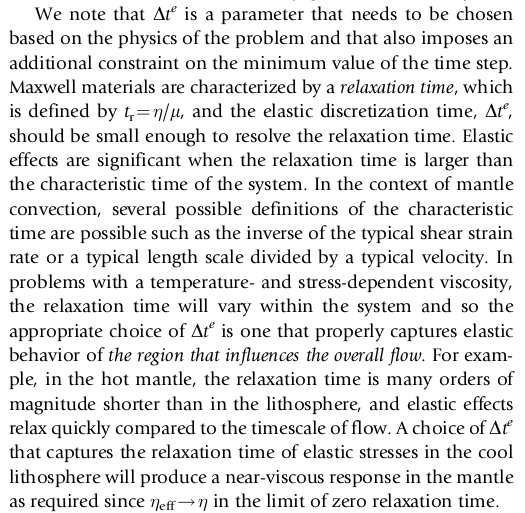
\includegraphics[width=8.25cm]{images/viscoelasticity/zhym12_g}
\end{multicols}

\begin{multicols}{2}
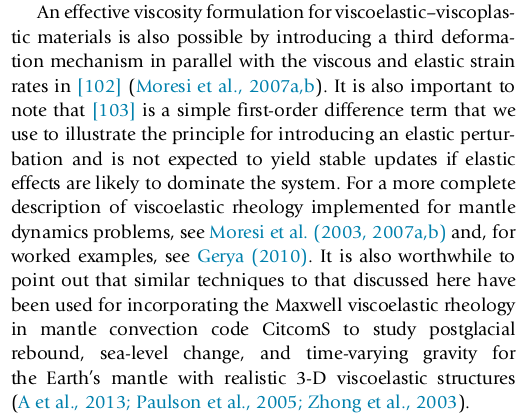
\includegraphics[width=8.25cm]{images/viscoelasticity/zhym12_h}
\end{multicols}


\newpage
\subsection{appendix: Equations in kemk13\label{ve_kemk13}} 
\fullcite{kemk13}

\begin{multicols}{2}
\begin{center}
{\bf Article excerpts}
\\ 
{\bf Notes and remarks}
\end{center}
\end{multicols}

%------------------------------------------------------------------------------

\begin{multicols}{2}
\includegraphics[width=8.4cm]{images/viscoelasticity/kemk13_a}
\end{multicols}

\begin{multicols}{2}
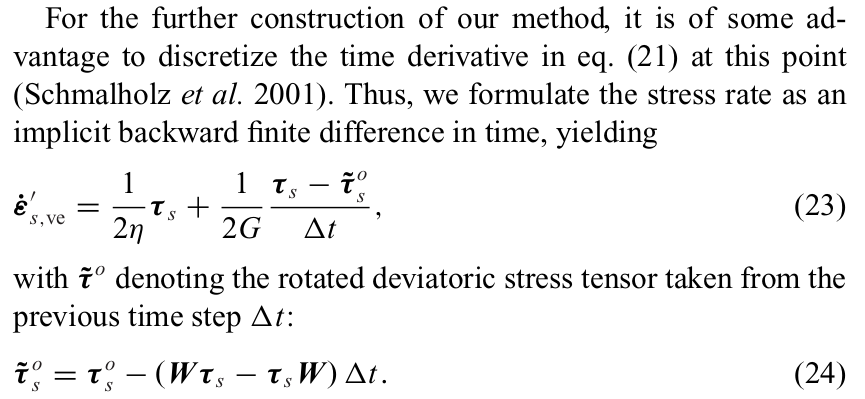
\includegraphics[width=8.4cm]{images/viscoelasticity/kemk13_b}
\end{multicols}

\begin{multicols}{2}
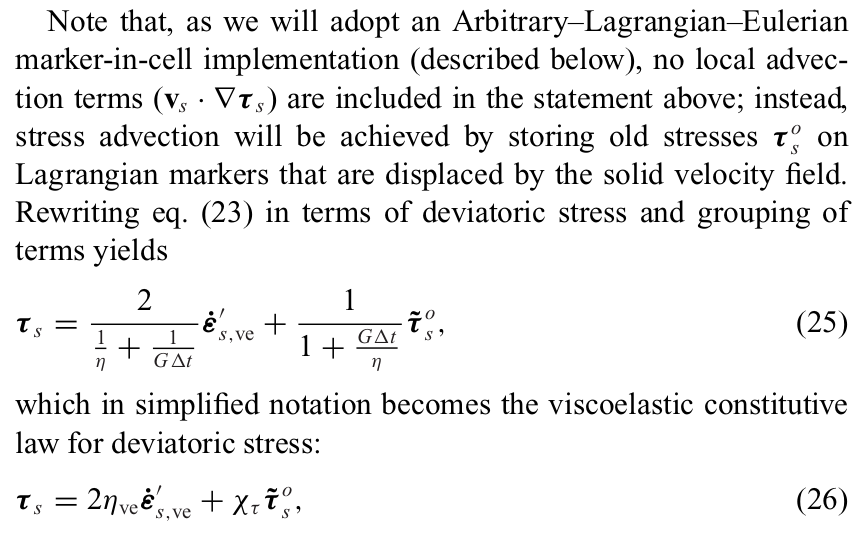
\includegraphics[width=8.4cm]{images/viscoelasticity/kemk13_c}
\end{multicols}

\begin{multicols}{2}
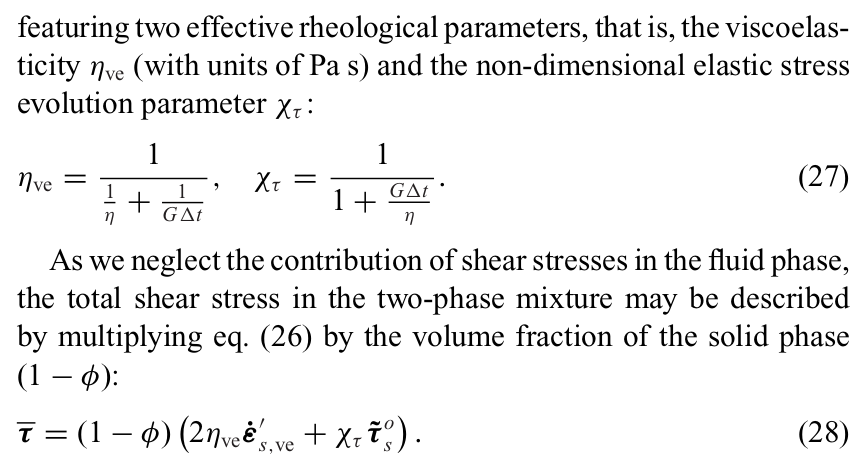
\includegraphics[width=8.4cm]{images/viscoelasticity/kemk13_d}
\end{multicols}


\newpage
\subsection{appendix: Equations in famc14\label{ve_famc14}} 
\fullcite{famc14}


\begin{multicols}{2}
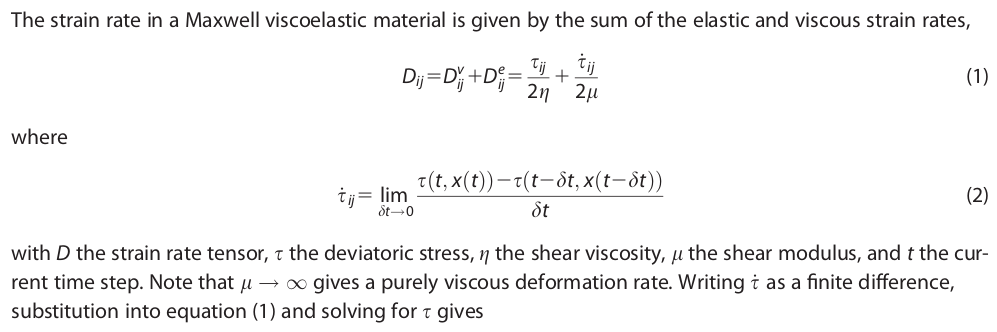
\includegraphics[width=8.3cm]{images/viscoelasticity/famc14_a}\\
\[
\dot{\bm\varepsilon} = 
\dot{\bm\varepsilon}^v +
\dot{\bm\varepsilon}^e = 
\frac{{\bm \tau}}{2\eta} + 
\frac{\dot{\bm \tau}}{2\mu} 
\]
\end{multicols}

\begin{multicols}{2}
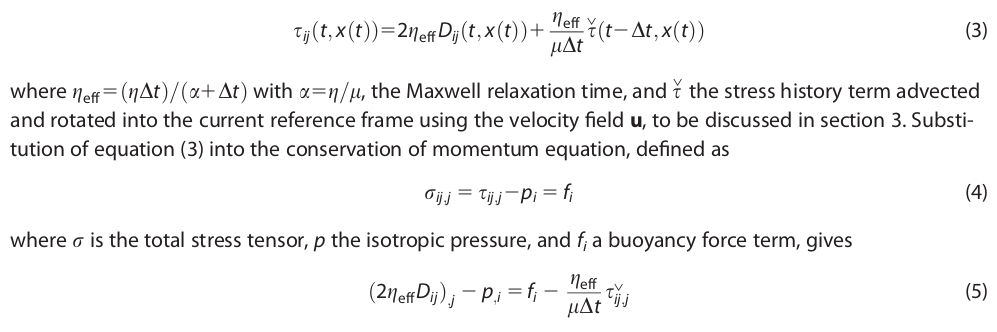
\includegraphics[width=8.3cm]{images/viscoelasticity/famc14_b}\\
\[
\vec\nabla\cdot (2 \eta_{ve} \dot{\bm\varepsilon}) - \vec\nabla p
= \vec{f} - ...
\]
\end{multicols}

\begin{multicols}{2}
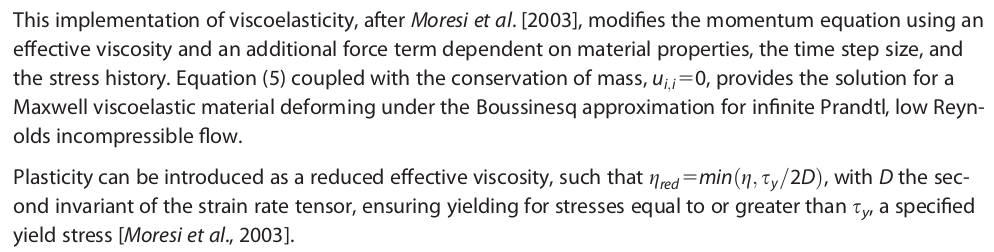
\includegraphics[width=8.3cm]{images/viscoelasticity/famc14_c}
\end{multicols}




\newpage
\subsection{appendix: Equations in vosc15\label{ve_vosc15}} 
\fullcite{vosc15}

This is a nice and technical article with a thorough description of the 
FEM discretisation. Added bonus, in 3d. 

\begin{multicols}{2}
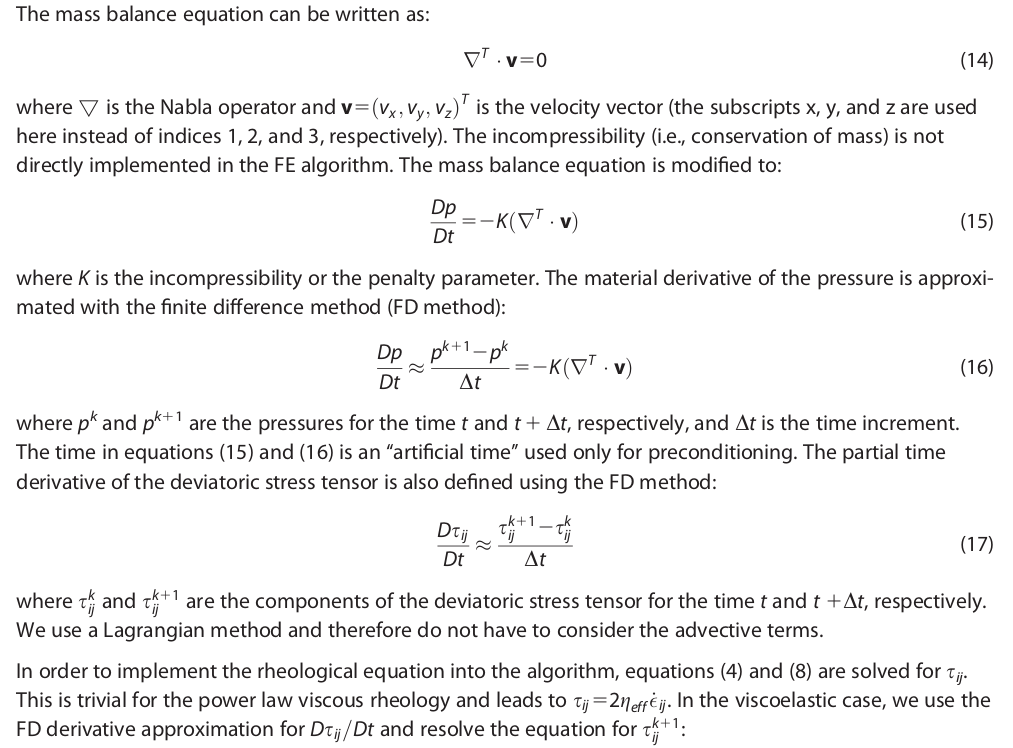
\includegraphics[width=8.25cm]{images/viscoelasticity/vosc15_l}\\
\[
\frac{Dp}{Dt} = -K \vec\nabla\cdot \vec\upnu
\]
\[
\frac{Dp}{Dt} \simeq \frac{p^{k+1} -p^k}{\delta t} = -K \vec\nabla\cdot \vec\upnu
\]
\end{multicols}

\begin{multicols}{2}
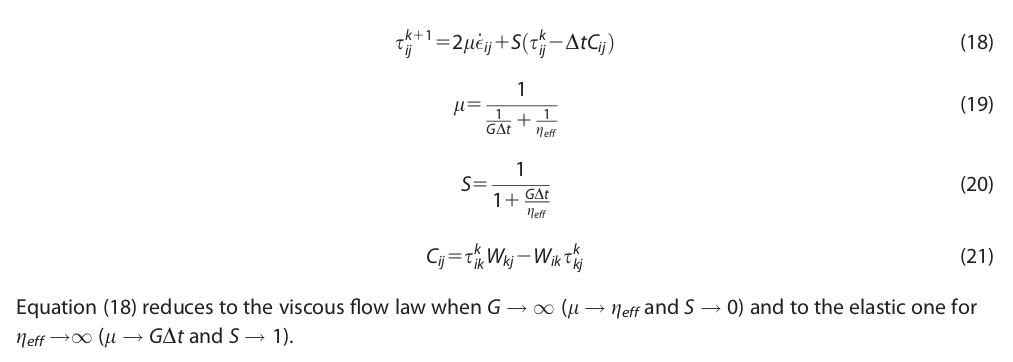
\includegraphics[width=8.25cm]{images/viscoelasticity/vosc15_m}\\
\[
\tau_{ij}^{k+1} = 2 \eta_{ve} \dot{\varepsilon}_{ij} + \left(1+\frac{G \delta t}{\eta}\right)^{-1} 
( \tau_{ij}^k - \tau^k_{ik} \omega_{kj} - \omega_{ik} \tau{kj}^k)
\]
with
\[
\eta_{ve}= \left(  \frac{1}{\eta} + \frac{1}{G \delta t} \right)^{-1}
\]

{\color{red} how to name S? }

\end{multicols}


\begin{multicols}{2}
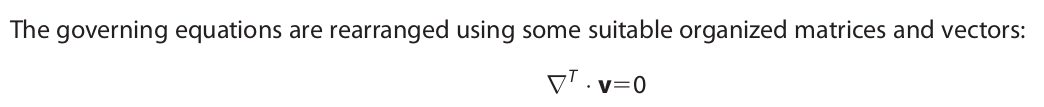
\includegraphics[width=8.25cm]{images/viscoelasticity/vosc15_a}\\
\[
\vec\nabla \cdot \vec\upnu = 0
\]
\end{multicols}

\begin{multicols}{2}
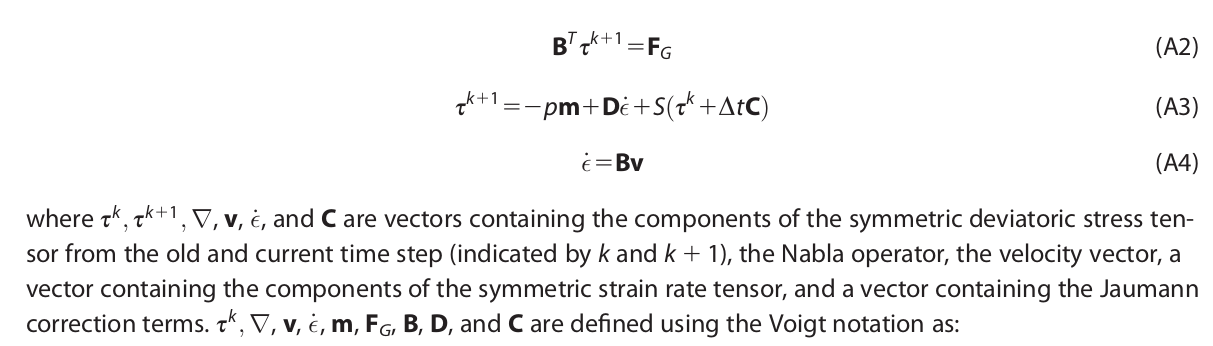
\includegraphics[width=8.25cm]{images/viscoelasticity/vosc15_b}\\
\[
\vec\tau^{k+1} = -p \vec{m}  + {\bm D} \cdot \vec{\varepsilon} 
+ S (\vec\tau^k + \delta t \; \vec{C})
\]
\end{multicols}

\begin{multicols}{2}
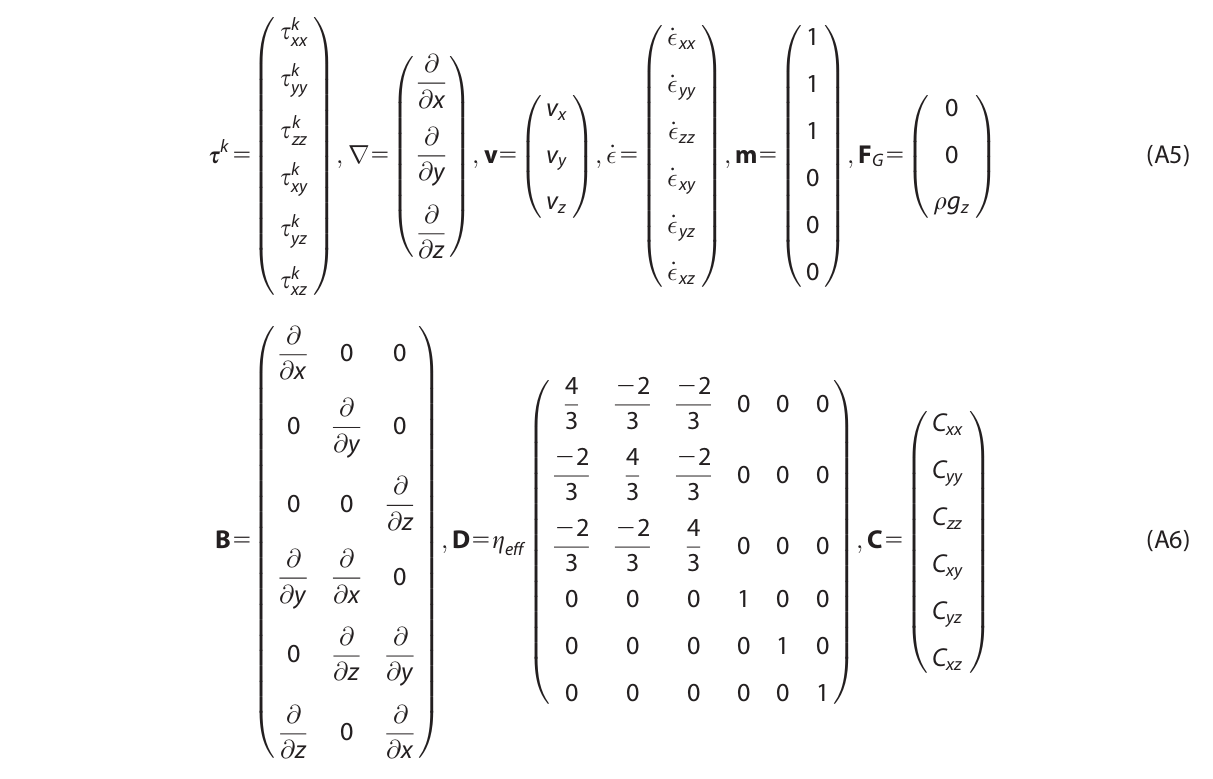
\includegraphics[width=8.25cm]{images/viscoelasticity/vosc15_c}
\end{multicols}

\begin{multicols}{2}
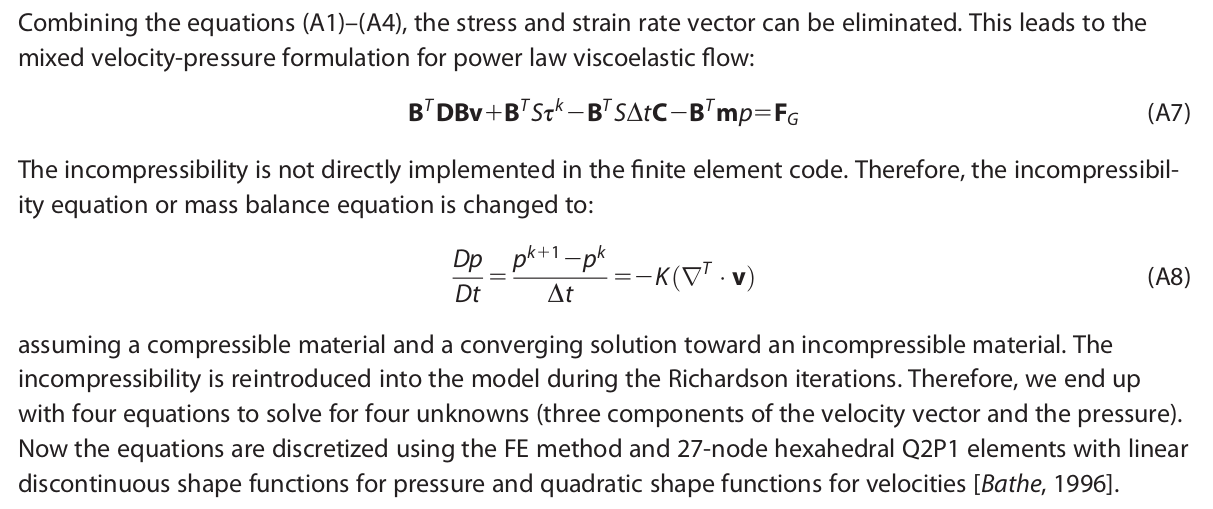
\includegraphics[width=8.25cm]{images/viscoelasticity/vosc15_d}
\end{multicols}


\begin{multicols}{2}
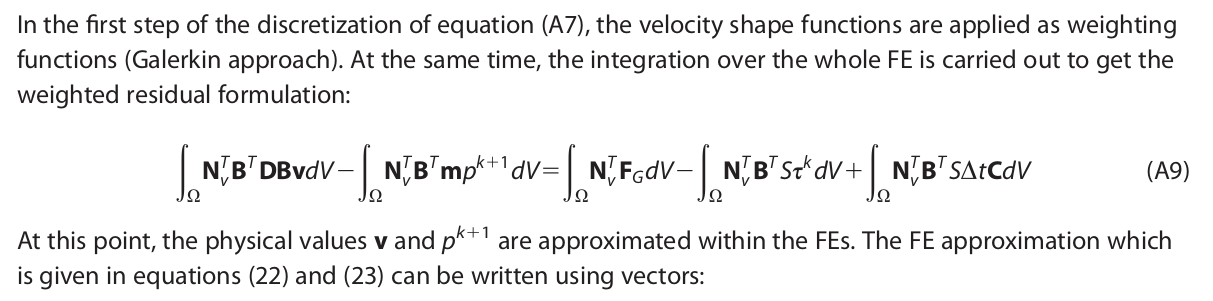
\includegraphics[width=8.25cm]{images/viscoelasticity/vosc15_e}
\end{multicols}

\begin{multicols}{2}
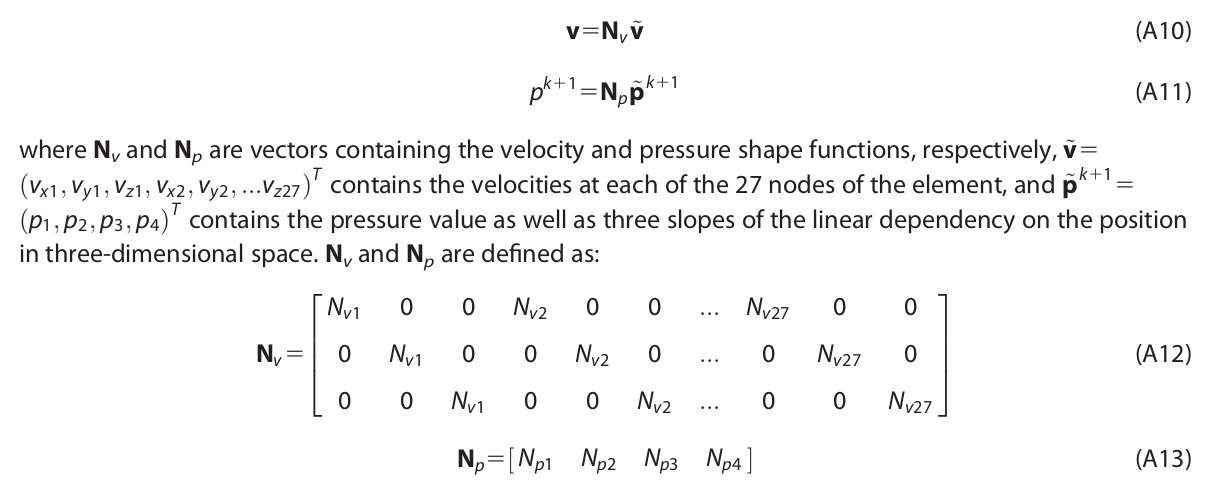
\includegraphics[width=8.25cm]{images/viscoelasticity/vosc15_f}
\end{multicols}

\begin{multicols}{2}
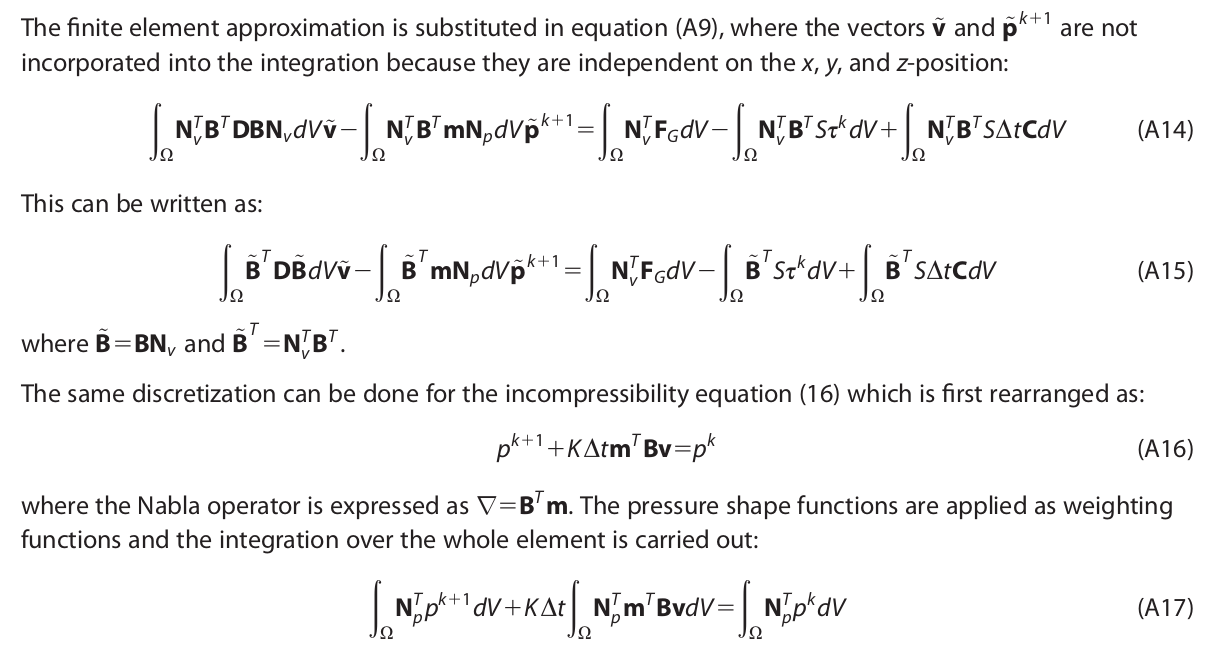
\includegraphics[width=8.25cm]{images/viscoelasticity/vosc15_g}
\end{multicols}

\begin{multicols}{2}
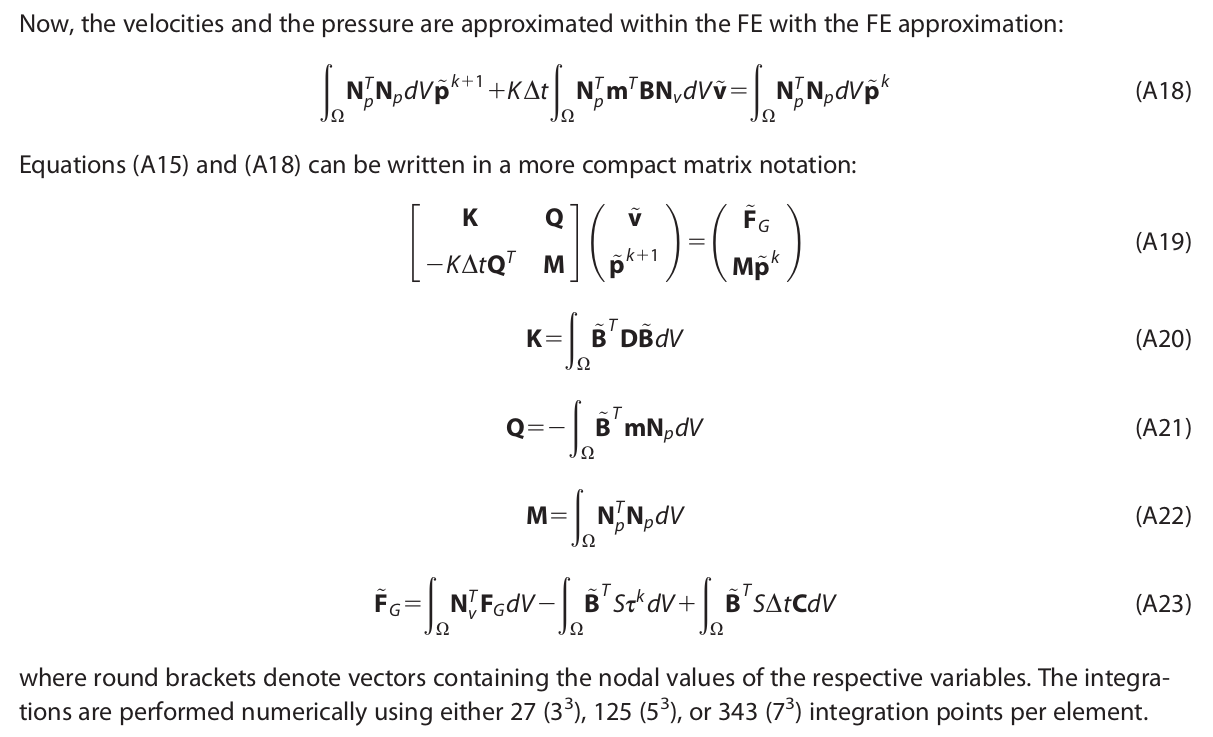
\includegraphics[width=8.25cm]{images/viscoelasticity/vosc15_h}
\end{multicols}

\begin{multicols}{2}
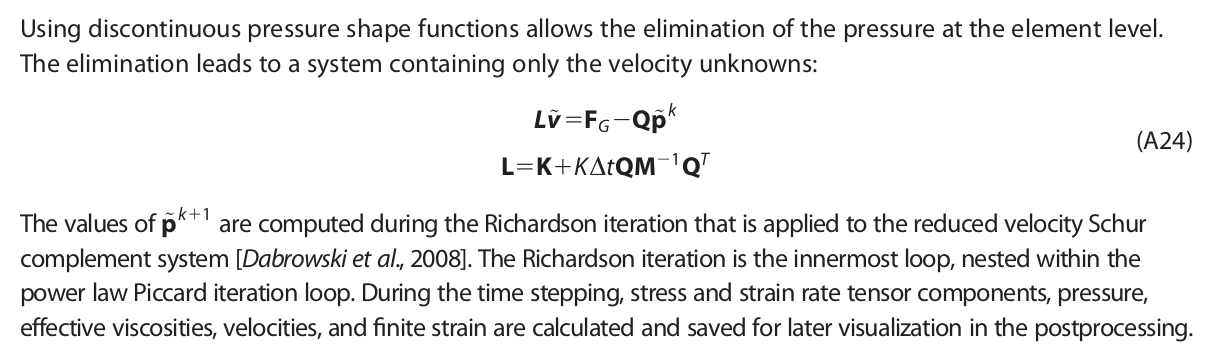
\includegraphics[width=8.25cm]{images/viscoelasticity/vosc15_i}
\end{multicols}








\newpage
\subsection{appendix: Equations in thkp15\label{ve_thkp15}} 
\fullcite{thkp15}

\begin{multicols}{2}
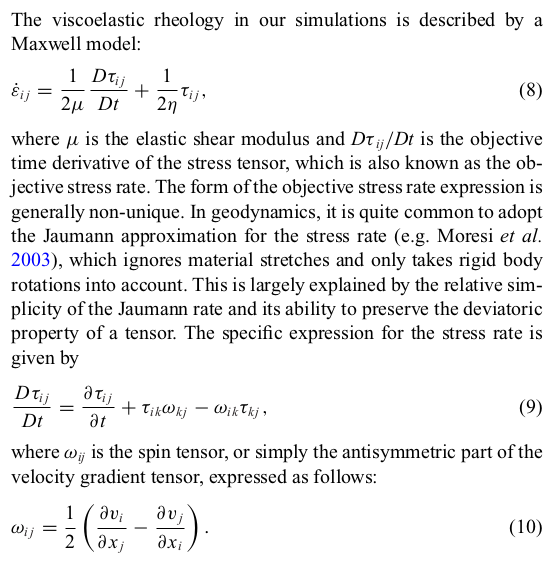
\includegraphics[width=8.25cm]{images/viscoelasticity/thkp15a}\\
\[
\dot{\bm\varepsilon} = 
\frac{1}{2\mu} \frac{{\cal D}{\bm \tau}}{{\cal D}t}
+\frac{1}{2\eta} {\bm \tau}
\]
Is is dev stress or full stress !?
\[
\frac{{\cal D} {\bm \tau}}{{\cal D}t} = 
\frac{\partial {\bm \tau}}{\partial t}  
+ {\bm \tau} \cdot \dot{\bm\omega} 
- \dot{\bm\omega} \cdot {\bm \tau}
\]
\end{multicols}

\begin{multicols}{2}
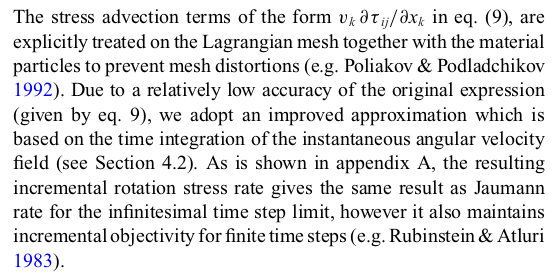
\includegraphics[width=8.25cm]{images/viscoelasticity/thkp15b}
\end{multicols}

\begin{multicols}{2}
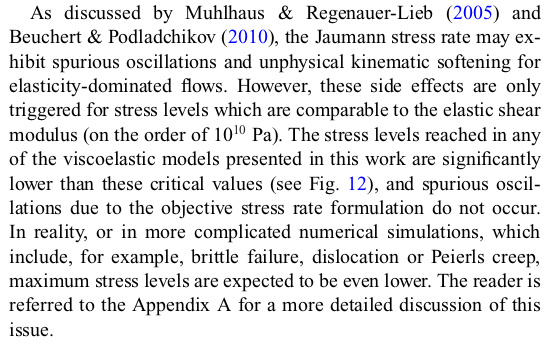
\includegraphics[width=8.25cm]{images/viscoelasticity/thkp15c}
\end{multicols}

\newpage
\paragraph{Discretization and solution}.

\begin{multicols}{2}
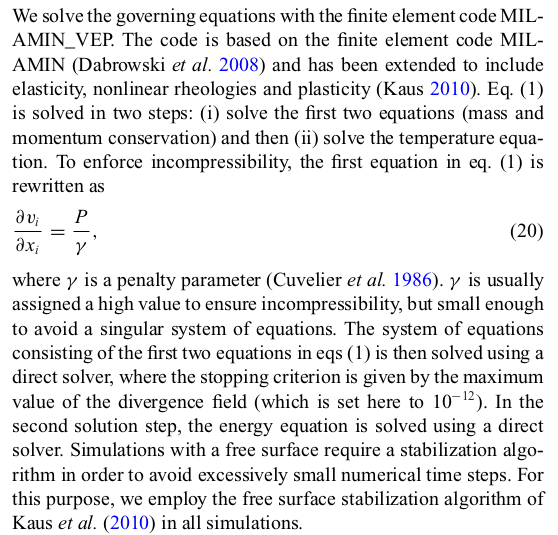
\includegraphics[width=8.25cm]{images/viscoelasticity/thkp15d}\\
\[
\vec\nabla\cdot \vec\upnu = \frac{1}{\lambda}p
\]
where $\lambda$ is a penalty parameter!
\end{multicols}

\begin{multicols}{2}
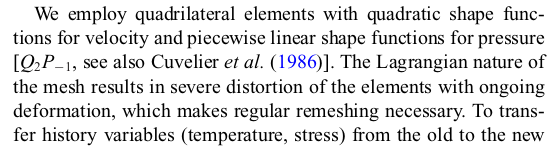
\includegraphics[width=8.25cm]{images/viscoelasticity/thkp15e}\\
$Q_2 \times P_{-1}$ element, discontinuous pressure field.
\end{multicols}

\begin{multicols}{2}
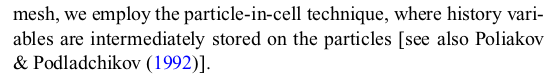
\includegraphics[width=8.25cm]{images/viscoelasticity/thkp15f}
\end{multicols}

\paragraph{Numerical formulation of viscoelasticity}.

\begin{multicols}{2}
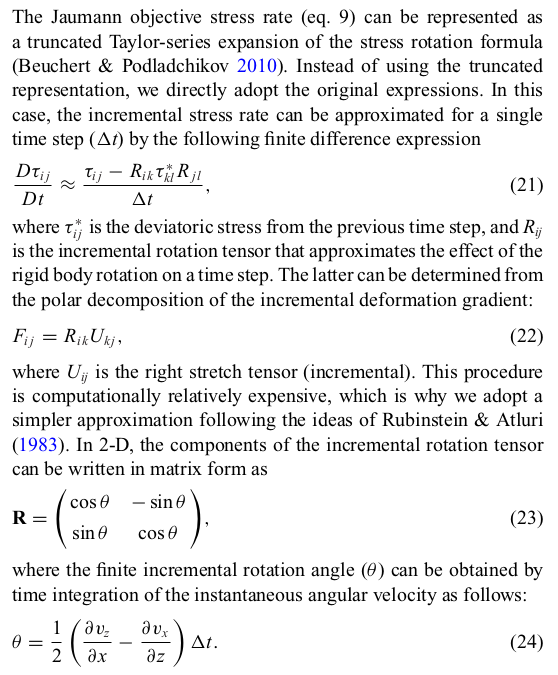
\includegraphics[width=8.25cm]{images/viscoelasticity/thkp15g}\\
\[
\frac{D \tau_{ij}^{k+1}}{Dt} \simeq \frac{\tau_{ij}^{k+1}- R_{ik}  \tau_{kl}^k R_{jl} }{\delta t}
\]
\[
{\bm R} = \left(\begin{array}{cc}
\cos\theta & -\sin \theta \\
\sin\theta & \cos\theta
\end{array}\right)
\]
\[
\theta = \frac12 \left(\frac{\partial v_z}{\partial x} - \frac{\partial v_x}{\partial z} \right) \delta t
\]
\end{multicols}

\begin{multicols}{2}
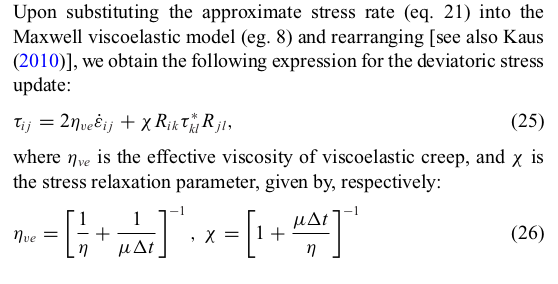
\includegraphics[width=8.25cm]{images/viscoelasticity/thkp15h}\\
\[
{\bm\tau}_{ij}^{k+1} = 2 \eta_{ve} \dot{\varepsilon}_{ij} + \xi R_{ik}  \tau_{kl}^k R_{jl} 
\]
with 
\[
\eta_{ve} = 
\left(
\frac{1}{\eta} + \frac{1}{\mu \delta t}
\right)^{-1}
\qquad
\xi = 
\left(
1 + \frac{\mu\delta t}{\eta}
\right)^{-1}
\]
\end{multicols}











\newpage
\subsection{appendix: Equations in daws16\label{ve_daws16}} 
\fullcite{daws16}

\begin{multicols}{2}
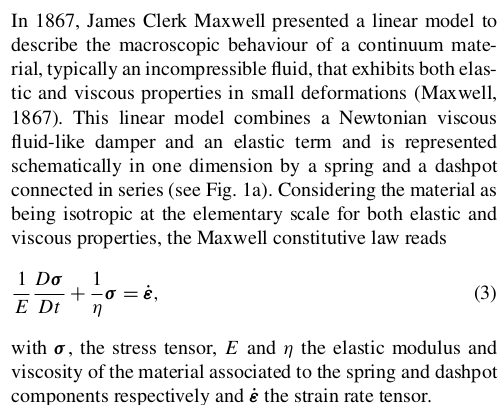
\includegraphics[width=8.25cm]{images/viscoelasticity/daws16a}\\
\[
\frac{1}{E} \frac{D{\bm \sigma}}{Dt} + \frac{1}{\eta} {\bm \sigma} = \dot{\bm\varepsilon}
\]
in 1d ?
\end{multicols}

\begin{multicols}{2}
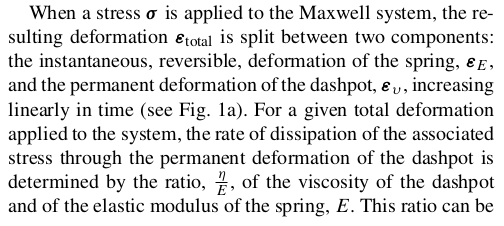
\includegraphics[width=8.25cm]{images/viscoelasticity/daws16b}
\end{multicols}

\begin{multicols}{2}
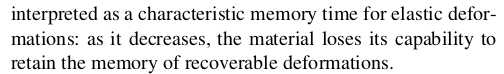
\includegraphics[width=8.25cm]{images/viscoelasticity/daws16c}
\end{multicols}

\begin{multicols}{2}
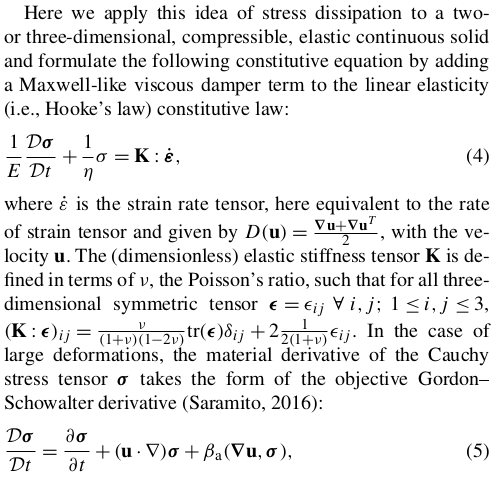
\includegraphics[width=8.25cm]{images/viscoelasticity/daws16f}\\
\[
\frac{1}{E} \frac{D{\bm \sigma}}{D t} + \frac{1}{\eta} \sigma 
= {\cal C}: \dot{\bm \varepsilon}
\]
with
\[
{\cal C}: \dot{\bm \varepsilon}
= \frac{\nu}{(1+\nu)(1-2\nu)} {\rm tr}({\bm \varepsilon}) {\bm 1}
+ 2\frac{1}{2(1+\nu)} {\bm \varepsilon}
\]

Gordon-Schowalter derivative:
\[
\frac{D{\bm \sigma}}{D t} = \frac{\partial{\bm \sigma}}{\partial t}
+ (\vec\upnu \cdot \vec\nabla) {\bm \sigma} +
\beta_a (\vec\nabla\vec\upnu,{\bm \sigma})
\]

\end{multicols}

\newpage

\begin{multicols}{2}
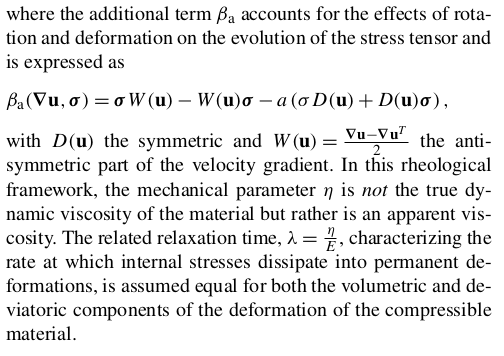
\includegraphics[width=8.25cm]{images/viscoelasticity/daws16d} \\
\[
\beta_a (\vec\nabla\vec\upnu,{\bm \sigma})
= {\bm \sigma}\cdot \dot{\bm \omega} - \dot{\bm \omega}\cdot {\bm \sigma}
- a ( {\bm \sigma} \cdot \dot{\bm \varepsilon}
+ \dot{\bm \varepsilon} \cdot {\bm \sigma})
\]
\end{multicols}



\begin{center}
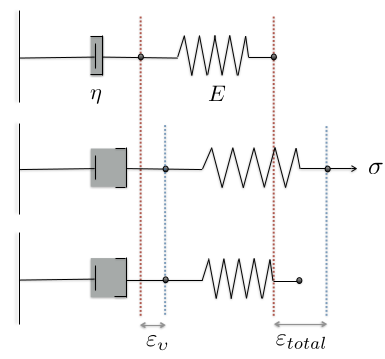
\includegraphics[width=8.25cm]{images/viscoelasticity/daws16e}\\
{\captionfont 
Schematic representations of the Maxwell model for a continuum material with 
elastic (shear) modulus $E$ and viscosity $\eta$. At time $t$, a stress is applied 
on the system. It is removed at time $t+\Delta t$: the spring goes back to its 
initial position but the dashpot retains its deformation $\varepsilon_v$.}
\end{center}















\newpage
\subsection{appendix: Equations in Gerya's book} 
iTaken from \fullcite{gery19book}

%.........................................
\paragraph{Rotation of elastic stresses}.

\begin{multicols}{2}
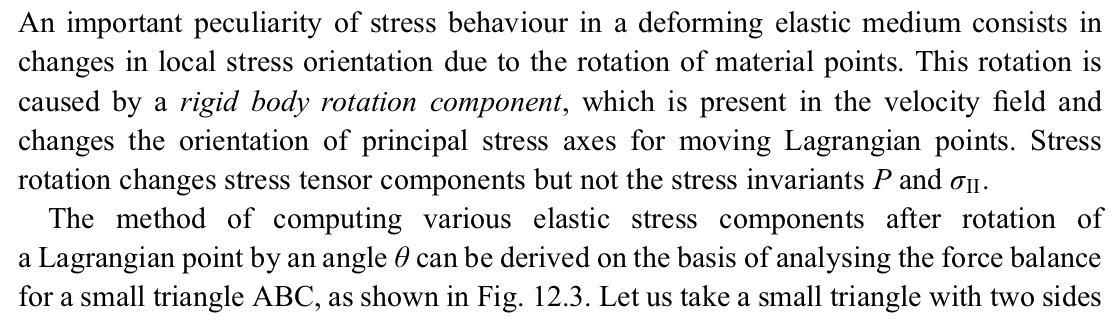
\includegraphics[width=8.3cm]{images/viscoelasticity/geryabook_1}
\end{multicols}

\begin{multicols}{2}
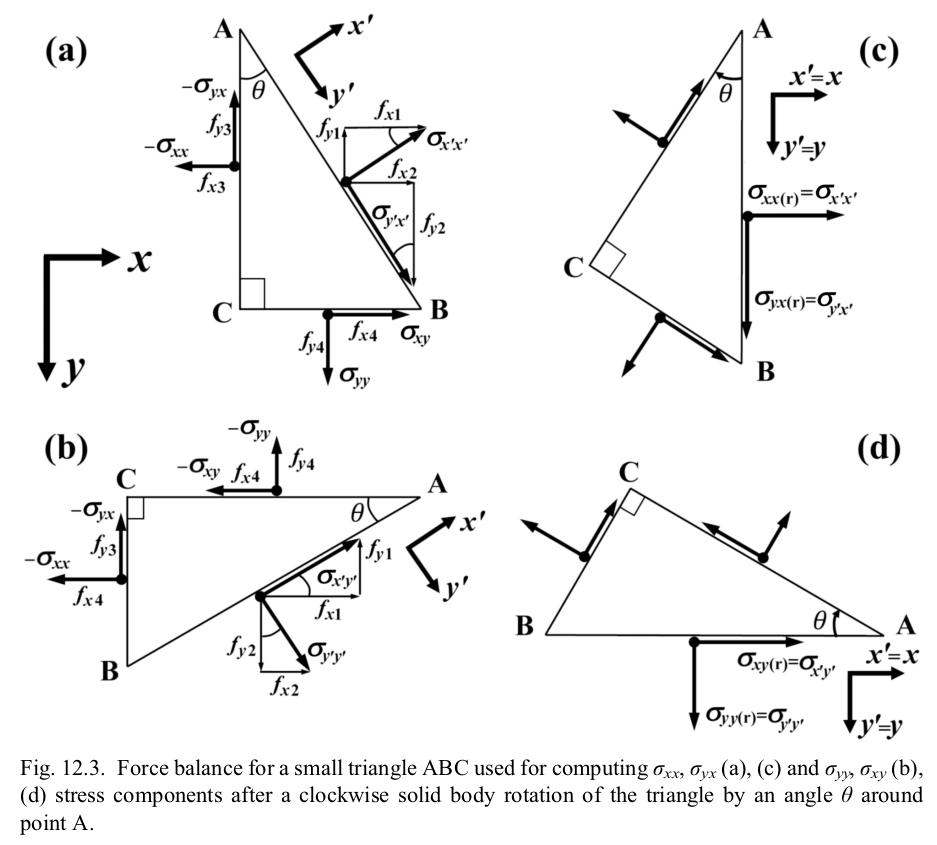
\includegraphics[width=8.3cm]{images/viscoelasticity/geryabook_19}
\end{multicols}

\begin{multicols}{2}
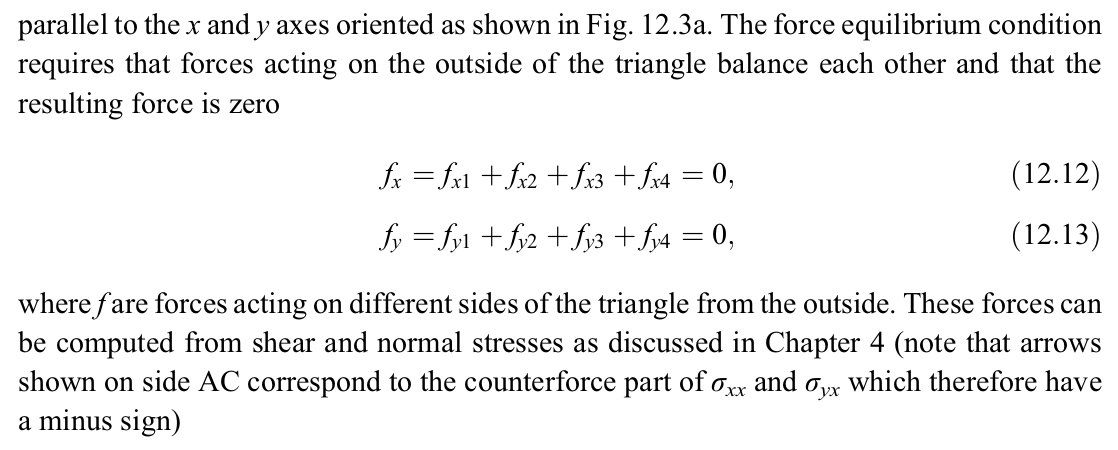
\includegraphics[width=8.3cm]{images/viscoelasticity/geryabook_2}
\end{multicols}

\begin{multicols}{2}
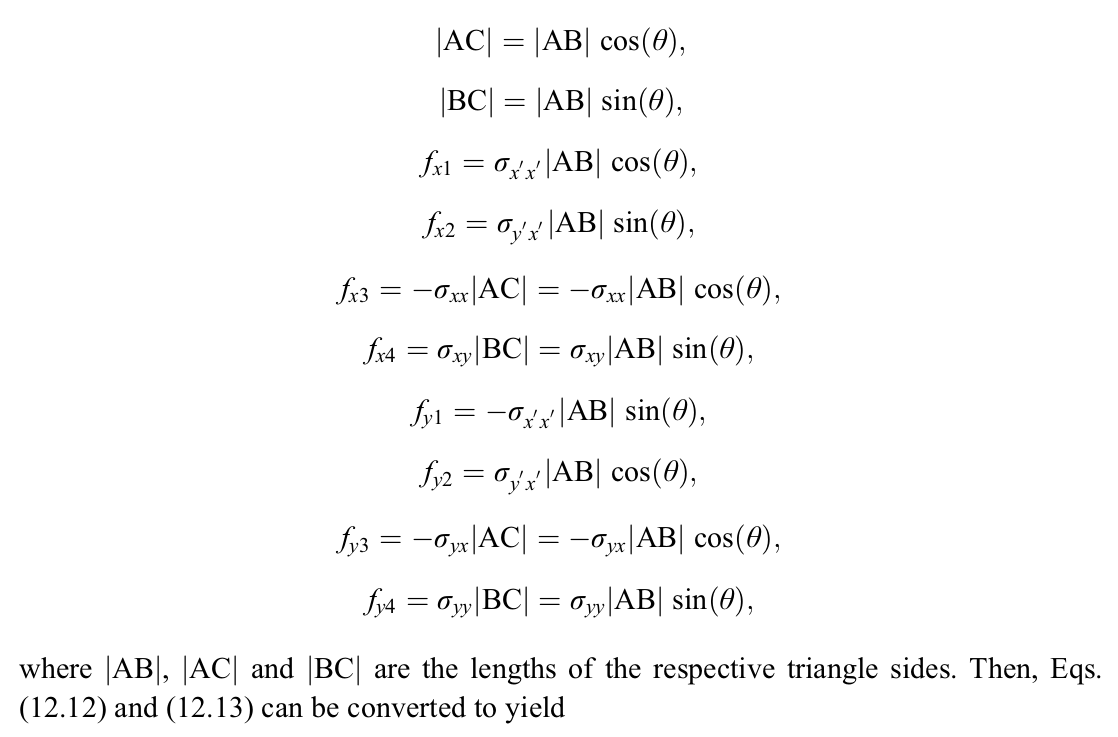
\includegraphics[width=8.3cm]{images/viscoelasticity/geryabook_3}
\end{multicols}

\begin{multicols}{2}
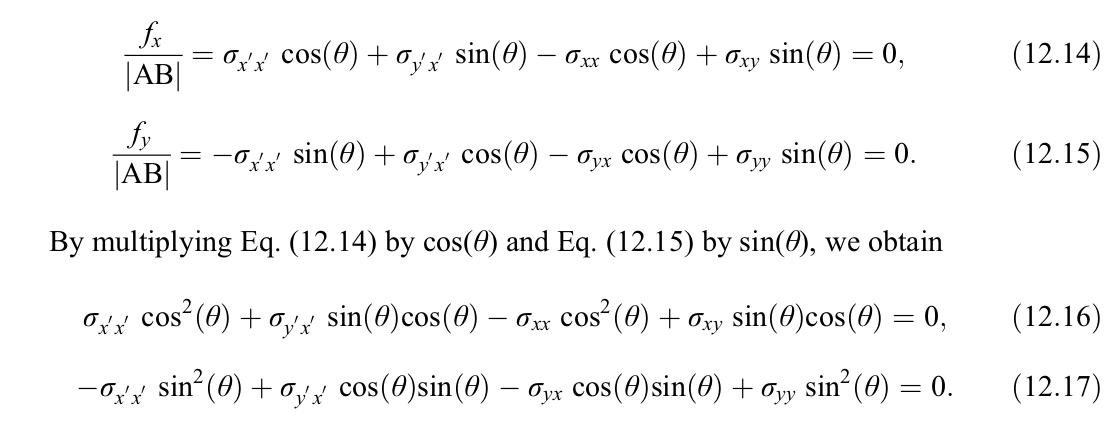
\includegraphics[width=8.3cm]{images/viscoelasticity/geryabook_4}
\end{multicols}

\begin{multicols}{2}
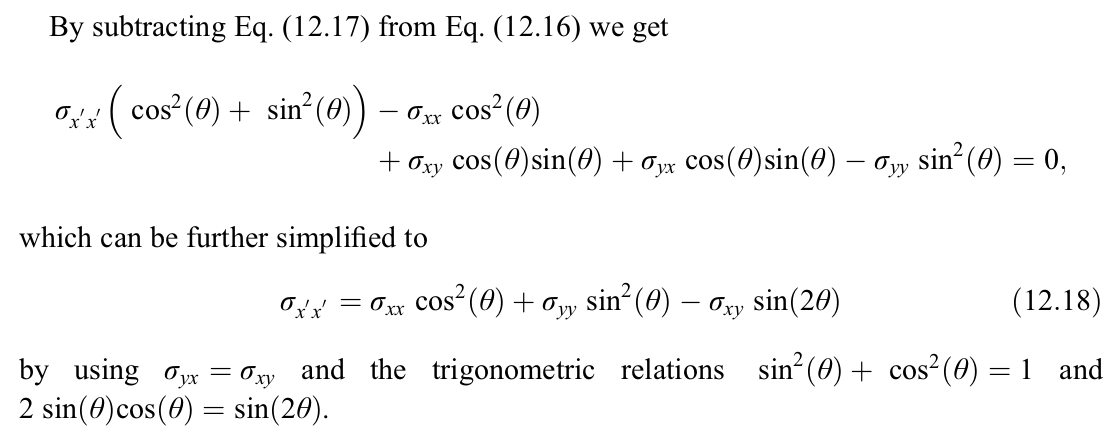
\includegraphics[width=8.3cm]{images/viscoelasticity/geryabook_5}
\end{multicols}

\begin{multicols}{2}
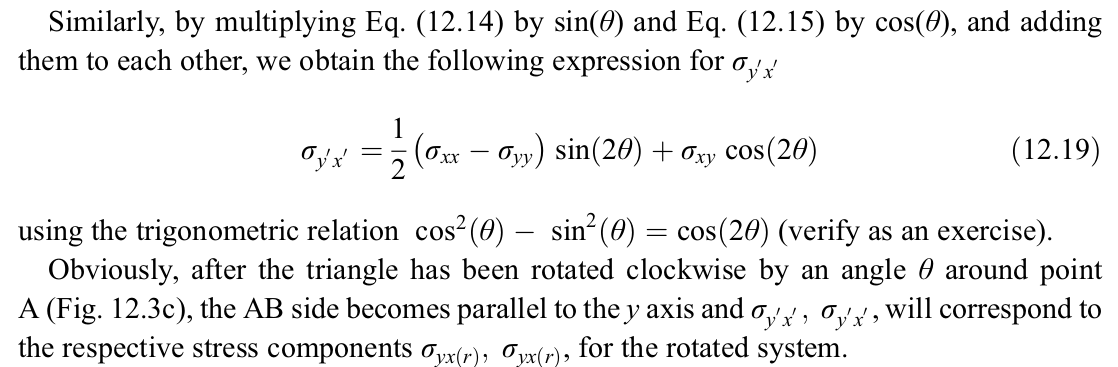
\includegraphics[width=8.3cm]{images/viscoelasticity/geryabook_6}
\end{multicols}

\begin{multicols}{2}
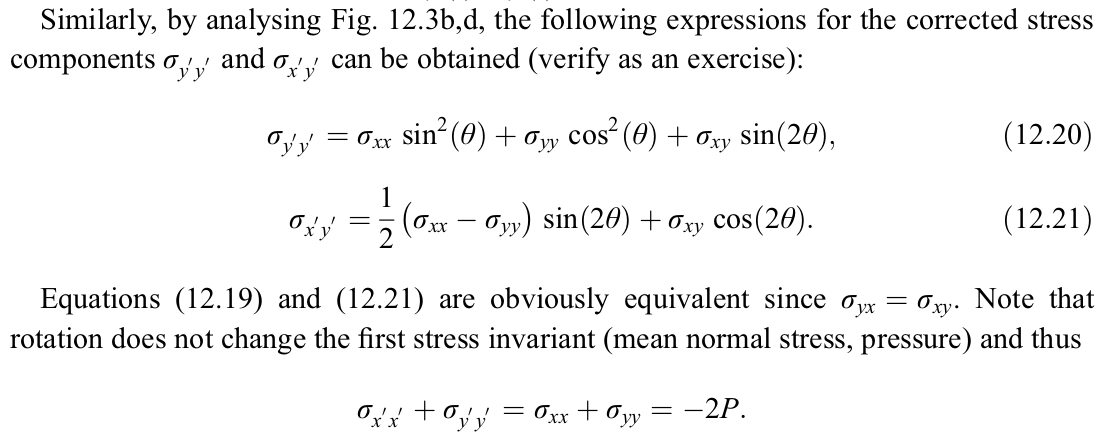
\includegraphics[width=8.3cm]{images/viscoelasticity/geryabook_7}
\end{multicols}

\begin{multicols}{2}
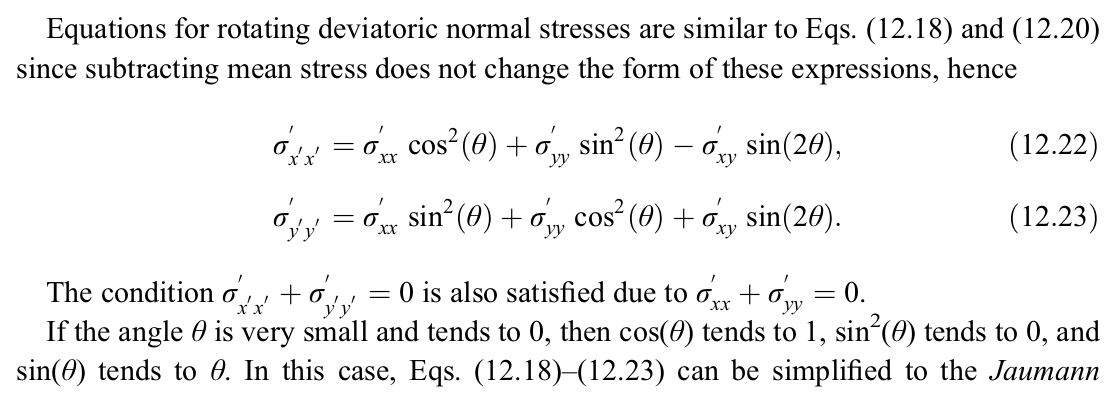
\includegraphics[width=8.3cm]{images/viscoelasticity/geryabook_8}
\end{multicols}

\begin{multicols}{2}
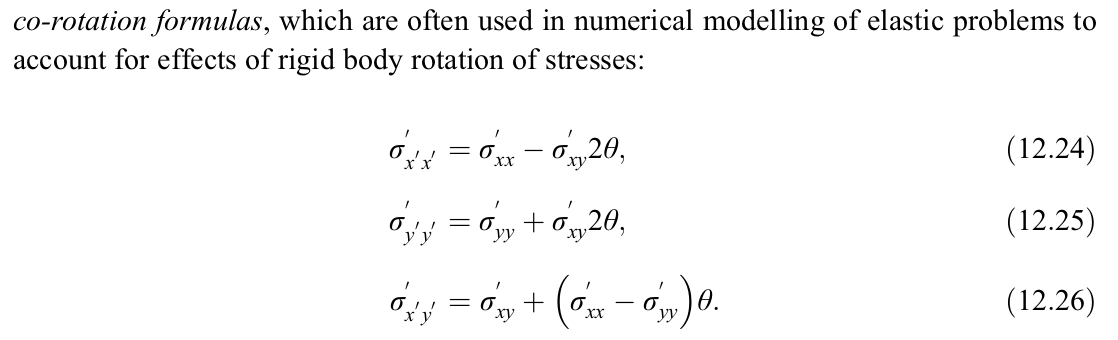
\includegraphics[width=8.3cm]{images/viscoelasticity/geryabook_9}
\end{multicols}

\begin{multicols}{2}
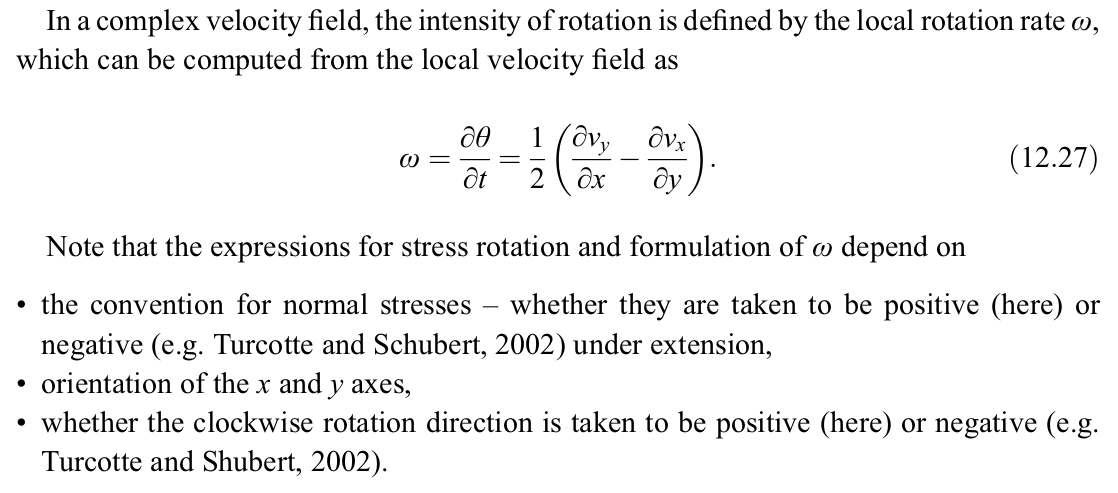
\includegraphics[width=8.3cm]{images/viscoelasticity/geryabook_10}
\end{multicols}

\begin{multicols}{2}
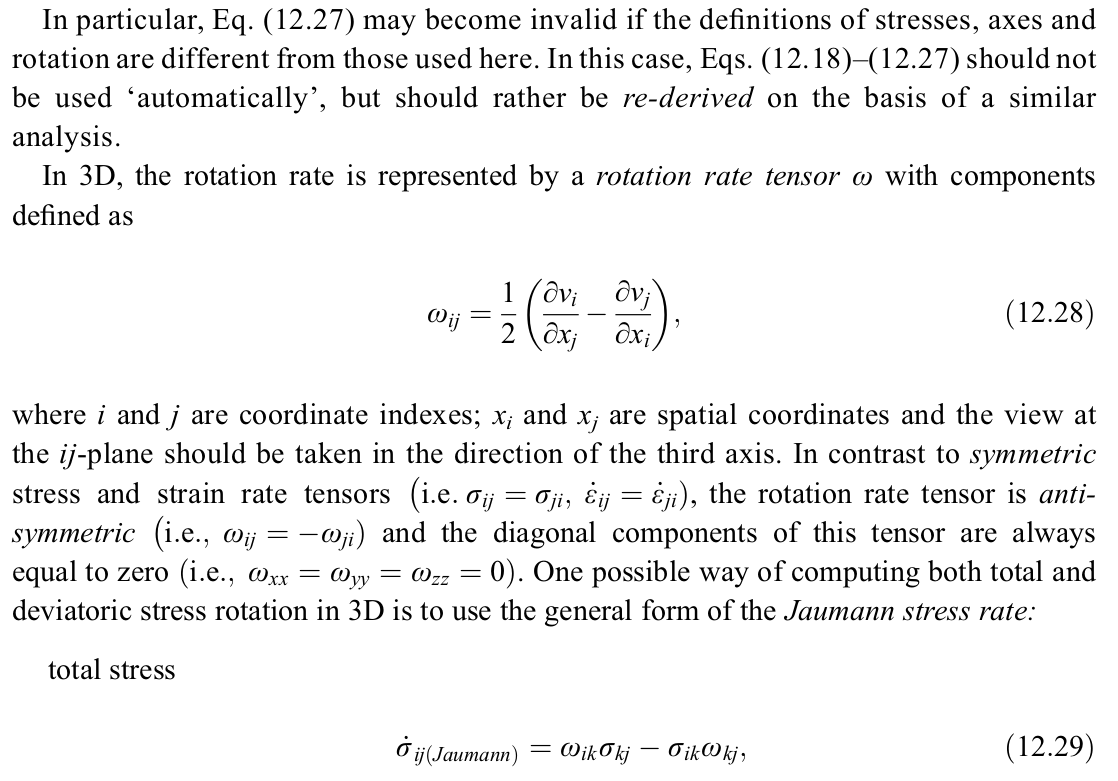
\includegraphics[width=8.3cm]{images/viscoelasticity/geryabook_11}
\end{multicols}

\begin{multicols}{2}
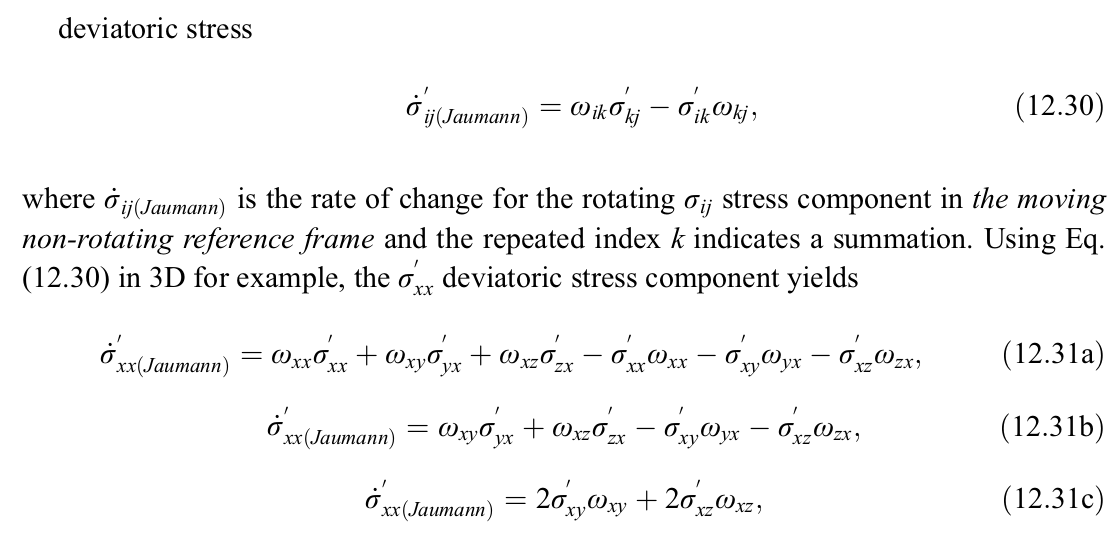
\includegraphics[width=8.3cm]{images/viscoelasticity/geryabook_12}
\end{multicols}

\begin{multicols}{2}
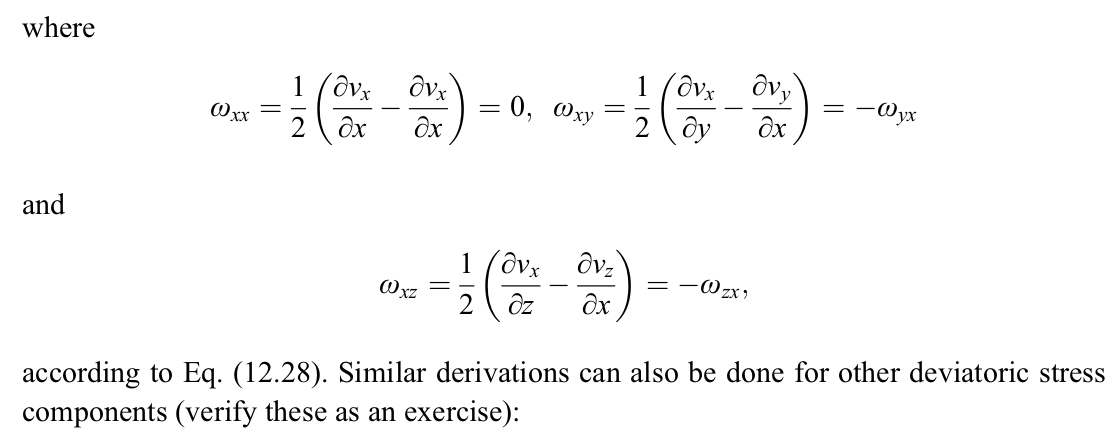
\includegraphics[width=8.3cm]{images/viscoelasticity/geryabook_13}
\end{multicols}

\begin{multicols}{2}
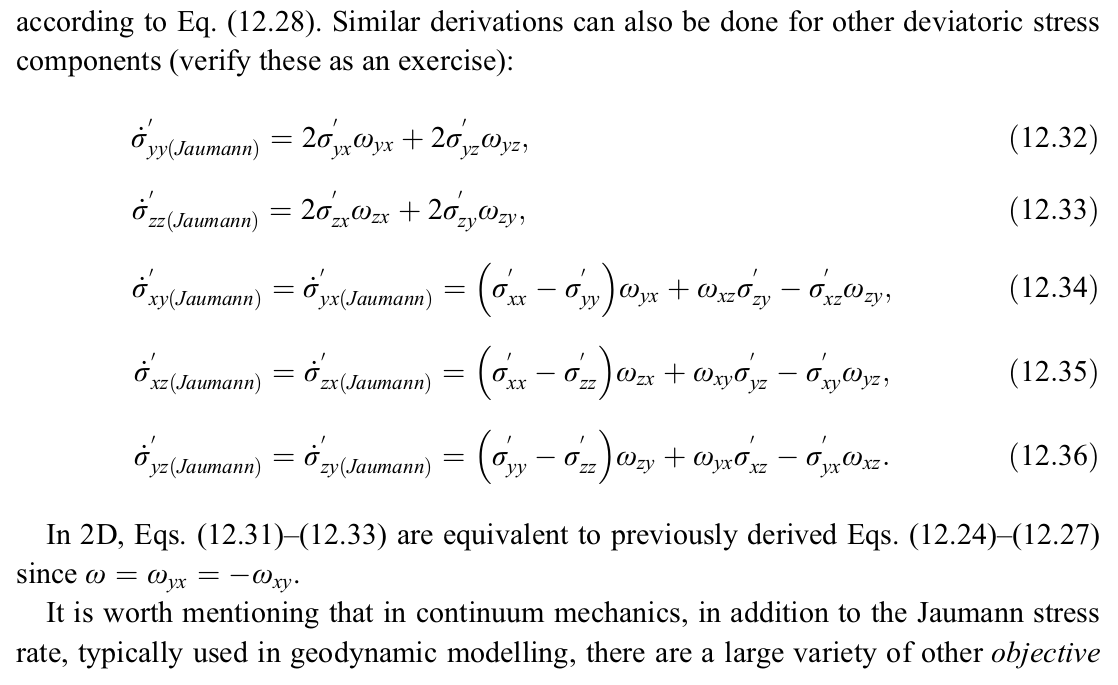
\includegraphics[width=8.3cm]{images/viscoelasticity/geryabook_14}
\end{multicols}

\begin{multicols}{2}
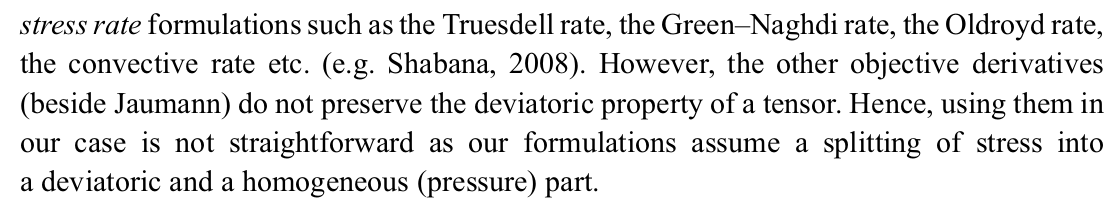
\includegraphics[width=8.3cm]{images/viscoelasticity/geryabook_15}
\end{multicols}

\begin{multicols}{2}
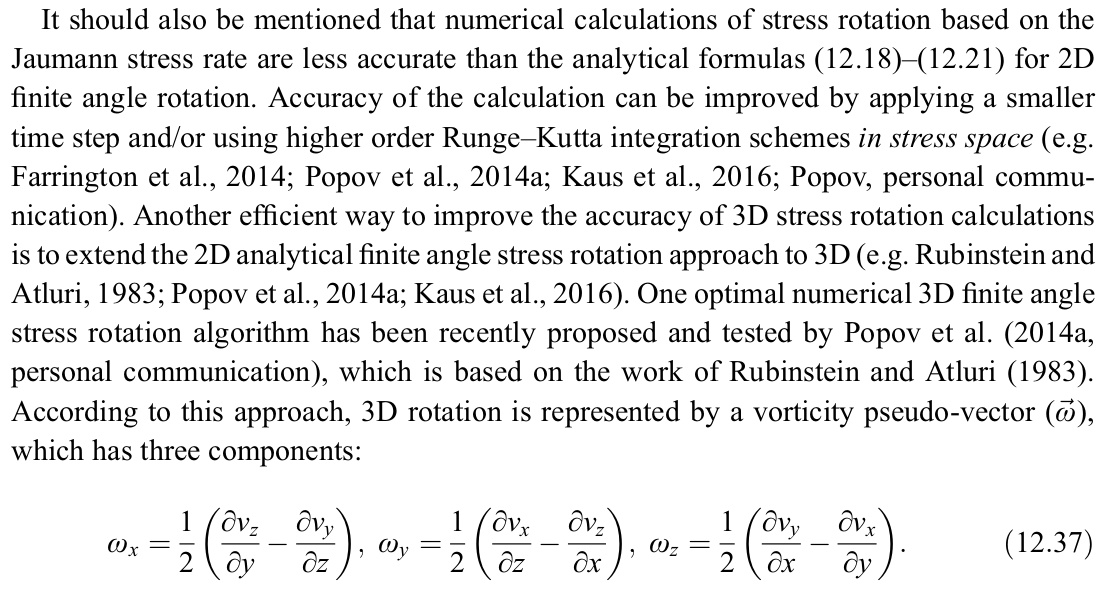
\includegraphics[width=8.3cm]{images/viscoelasticity/geryabook_16}
\end{multicols}

\begin{multicols}{2}
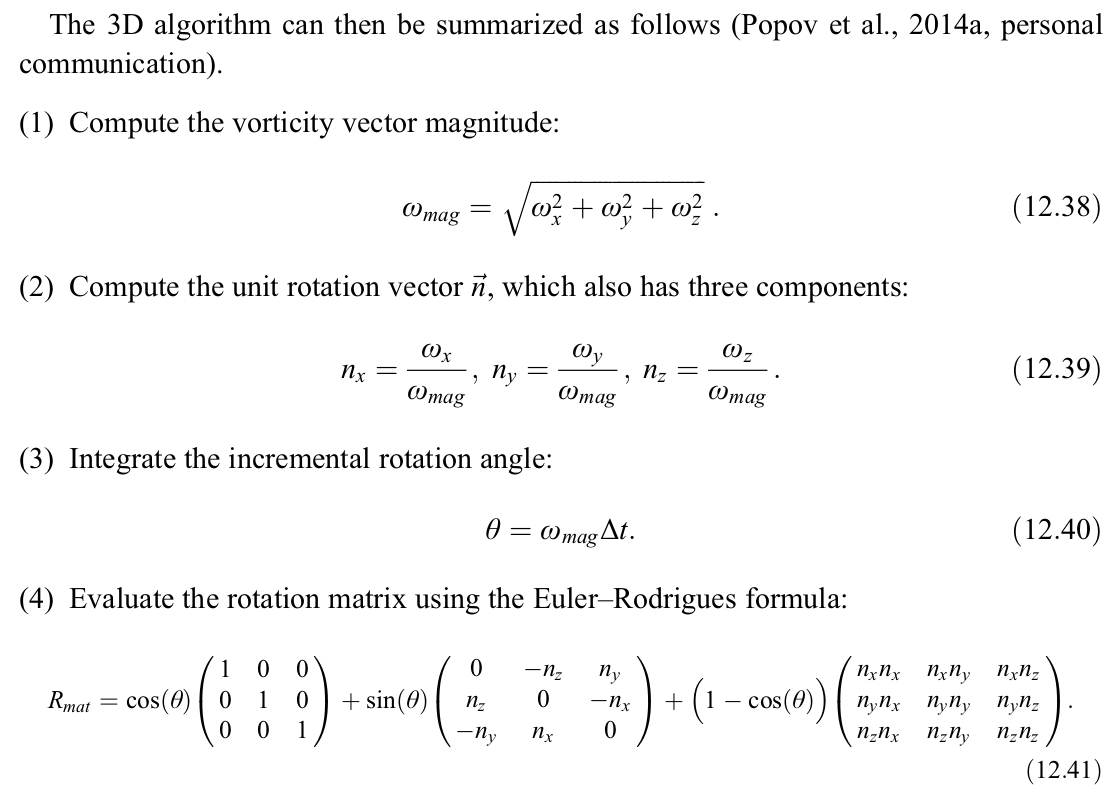
\includegraphics[width=8.3cm]{images/viscoelasticity/geryabook_17}
\end{multicols}

\begin{multicols}{2}
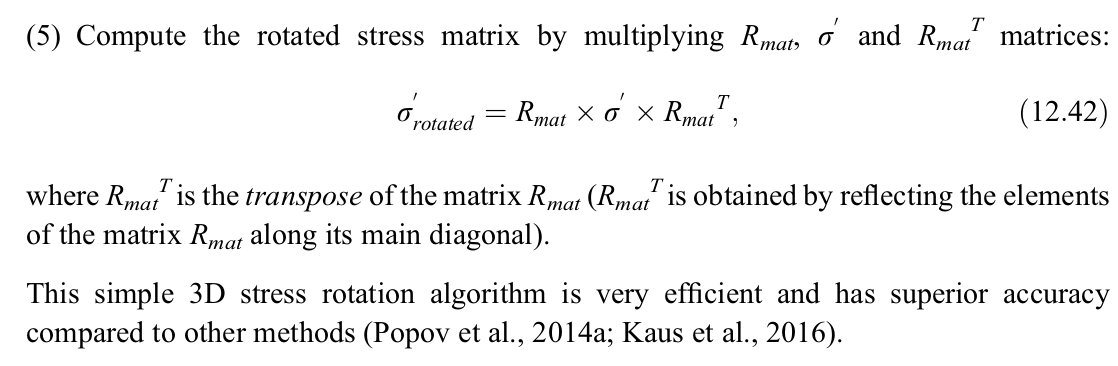
\includegraphics[width=8.3cm]{images/viscoelasticity/geryabook_18}
\end{multicols}

%.........................................
\paragraph{Maxwell visco-elastic rheology}.

\begin{multicols}{2}
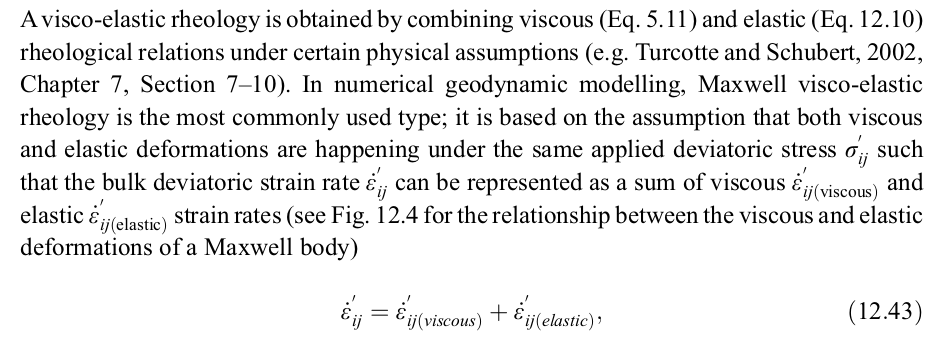
\includegraphics[width=8.3cm]{images/viscoelasticity/geryabook_20}
\end{multicols}

\begin{multicols}{2}
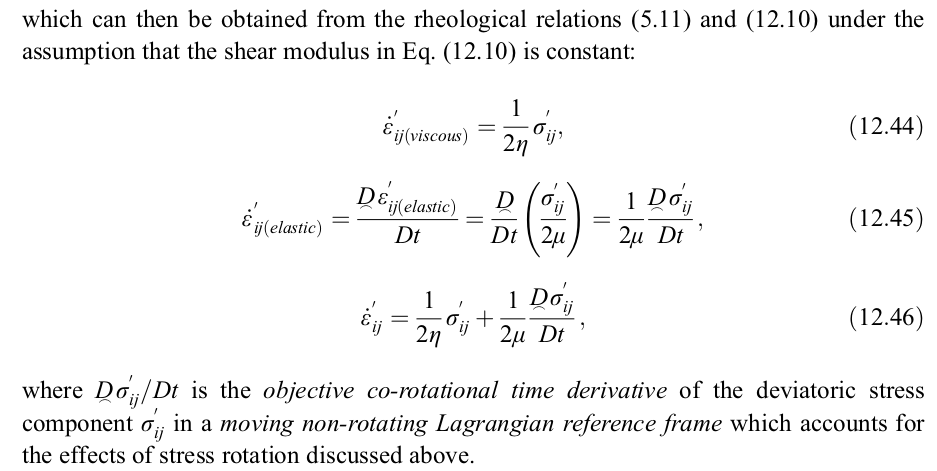
\includegraphics[width=8.3cm]{images/viscoelasticity/geryabook_21}
\end{multicols}

\begin{multicols}{2}
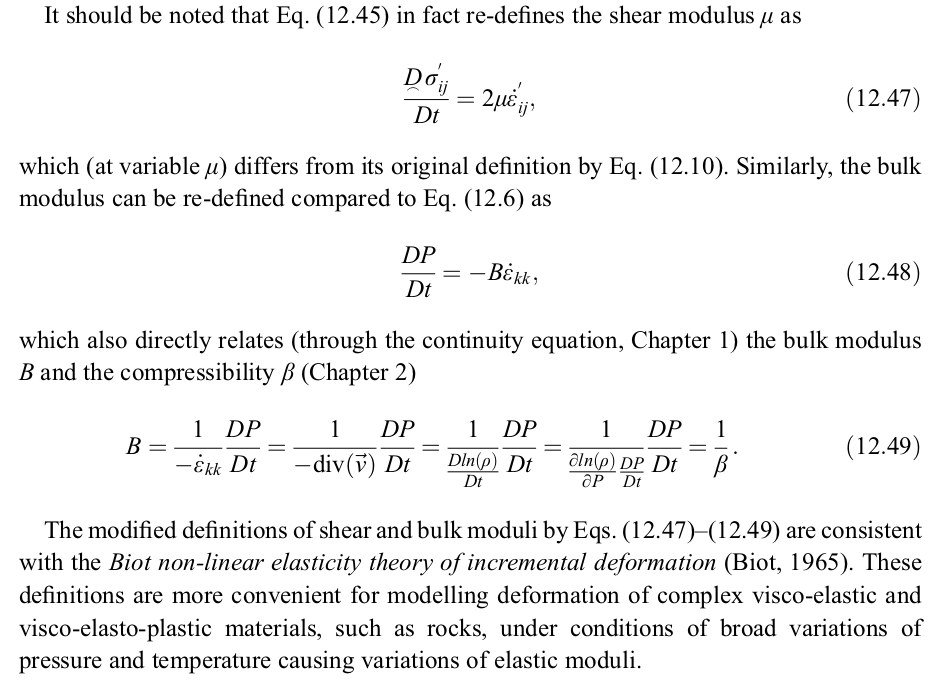
\includegraphics[width=8.3cm]{images/viscoelasticity/geryabook_22}
\end{multicols}






